%some-literature review


In the last few decades, several scientists have modeled the dynamics and ecological impact of  marine aggregates \cite{jackson_aggregation_1998, kiorboe_mechanisms_2002}. 
Their effects on bacterial transport \cite{jackson_simulation_1989} and algal bloom \cite{jackson_model_1990} have been described in models that use simplified descriptions of the aggregates' settling speeds. Moreover, accumulation of aggregates in thin layers where the ambient fluid is stratified have been reported \cite{macintyre_accumulation_1995, alldredge_occurrence_2002} and more recently modeled experimentally \cite{prairie_delayed_2013}, analytically \cite{camassa_retention_2013}, and computationally \cite{panah_simulations_2017}. Understanding the formation and persistence of these thin layers is ecologically important. 
Therefore, in this chapter, we discuss the dynamics of settling marine aggregates in a density stratified fluid. 
%---------------------------------------------------------
\par
Instead of constant density $\rho$, we suppose the background fluid density varies linearly in the vertical direction,
\begin{equation}
\rho_{bg}(z) =  \rho_0 \left(1 + \gamma z \right),
\label{eq_rho_bg}
\end{equation}
where $\rho_0$ is the minimum fluid density at rest, which is located at the top of the domain, and $\gamma$ is constant.
Over the time $t$, some perturbations, $C(\vec{y},t)$, occur due to the concentration, $\tilde{S}(\vec{y},t)$, difference between the background fluid and settling aggregate,
\begin{equation}
C(\vec{y}, t) =  \tilde{S}(\vec{y},t) - \rho_{bg}(z).
\label{eq_perturb_C}
\end{equation}
From equations (\ref{eq_rho_bg}) and (\ref{eq_perturb_C}), we can establish the fluid density variation over the time,
\begin{equation}
	\rho(\vec{y},t ) 
	= \rho_{bg}(z) +  \alpha \rho_0 C(\vec{y},t) 
	 = \rho_0 \left( 1 + \gamma z  + \alpha  C(\vec{y},t) \right),
\label{eq_density}
\end{equation}
where the non-zero constant $\alpha $ describes type of solute. Knowing that the concentration is the amount of mole per volume, the density of the fluid would differ by the type of solute or chemicals with the same amount of molecules.
\begin{figure}[ht]
	\begin{center}
	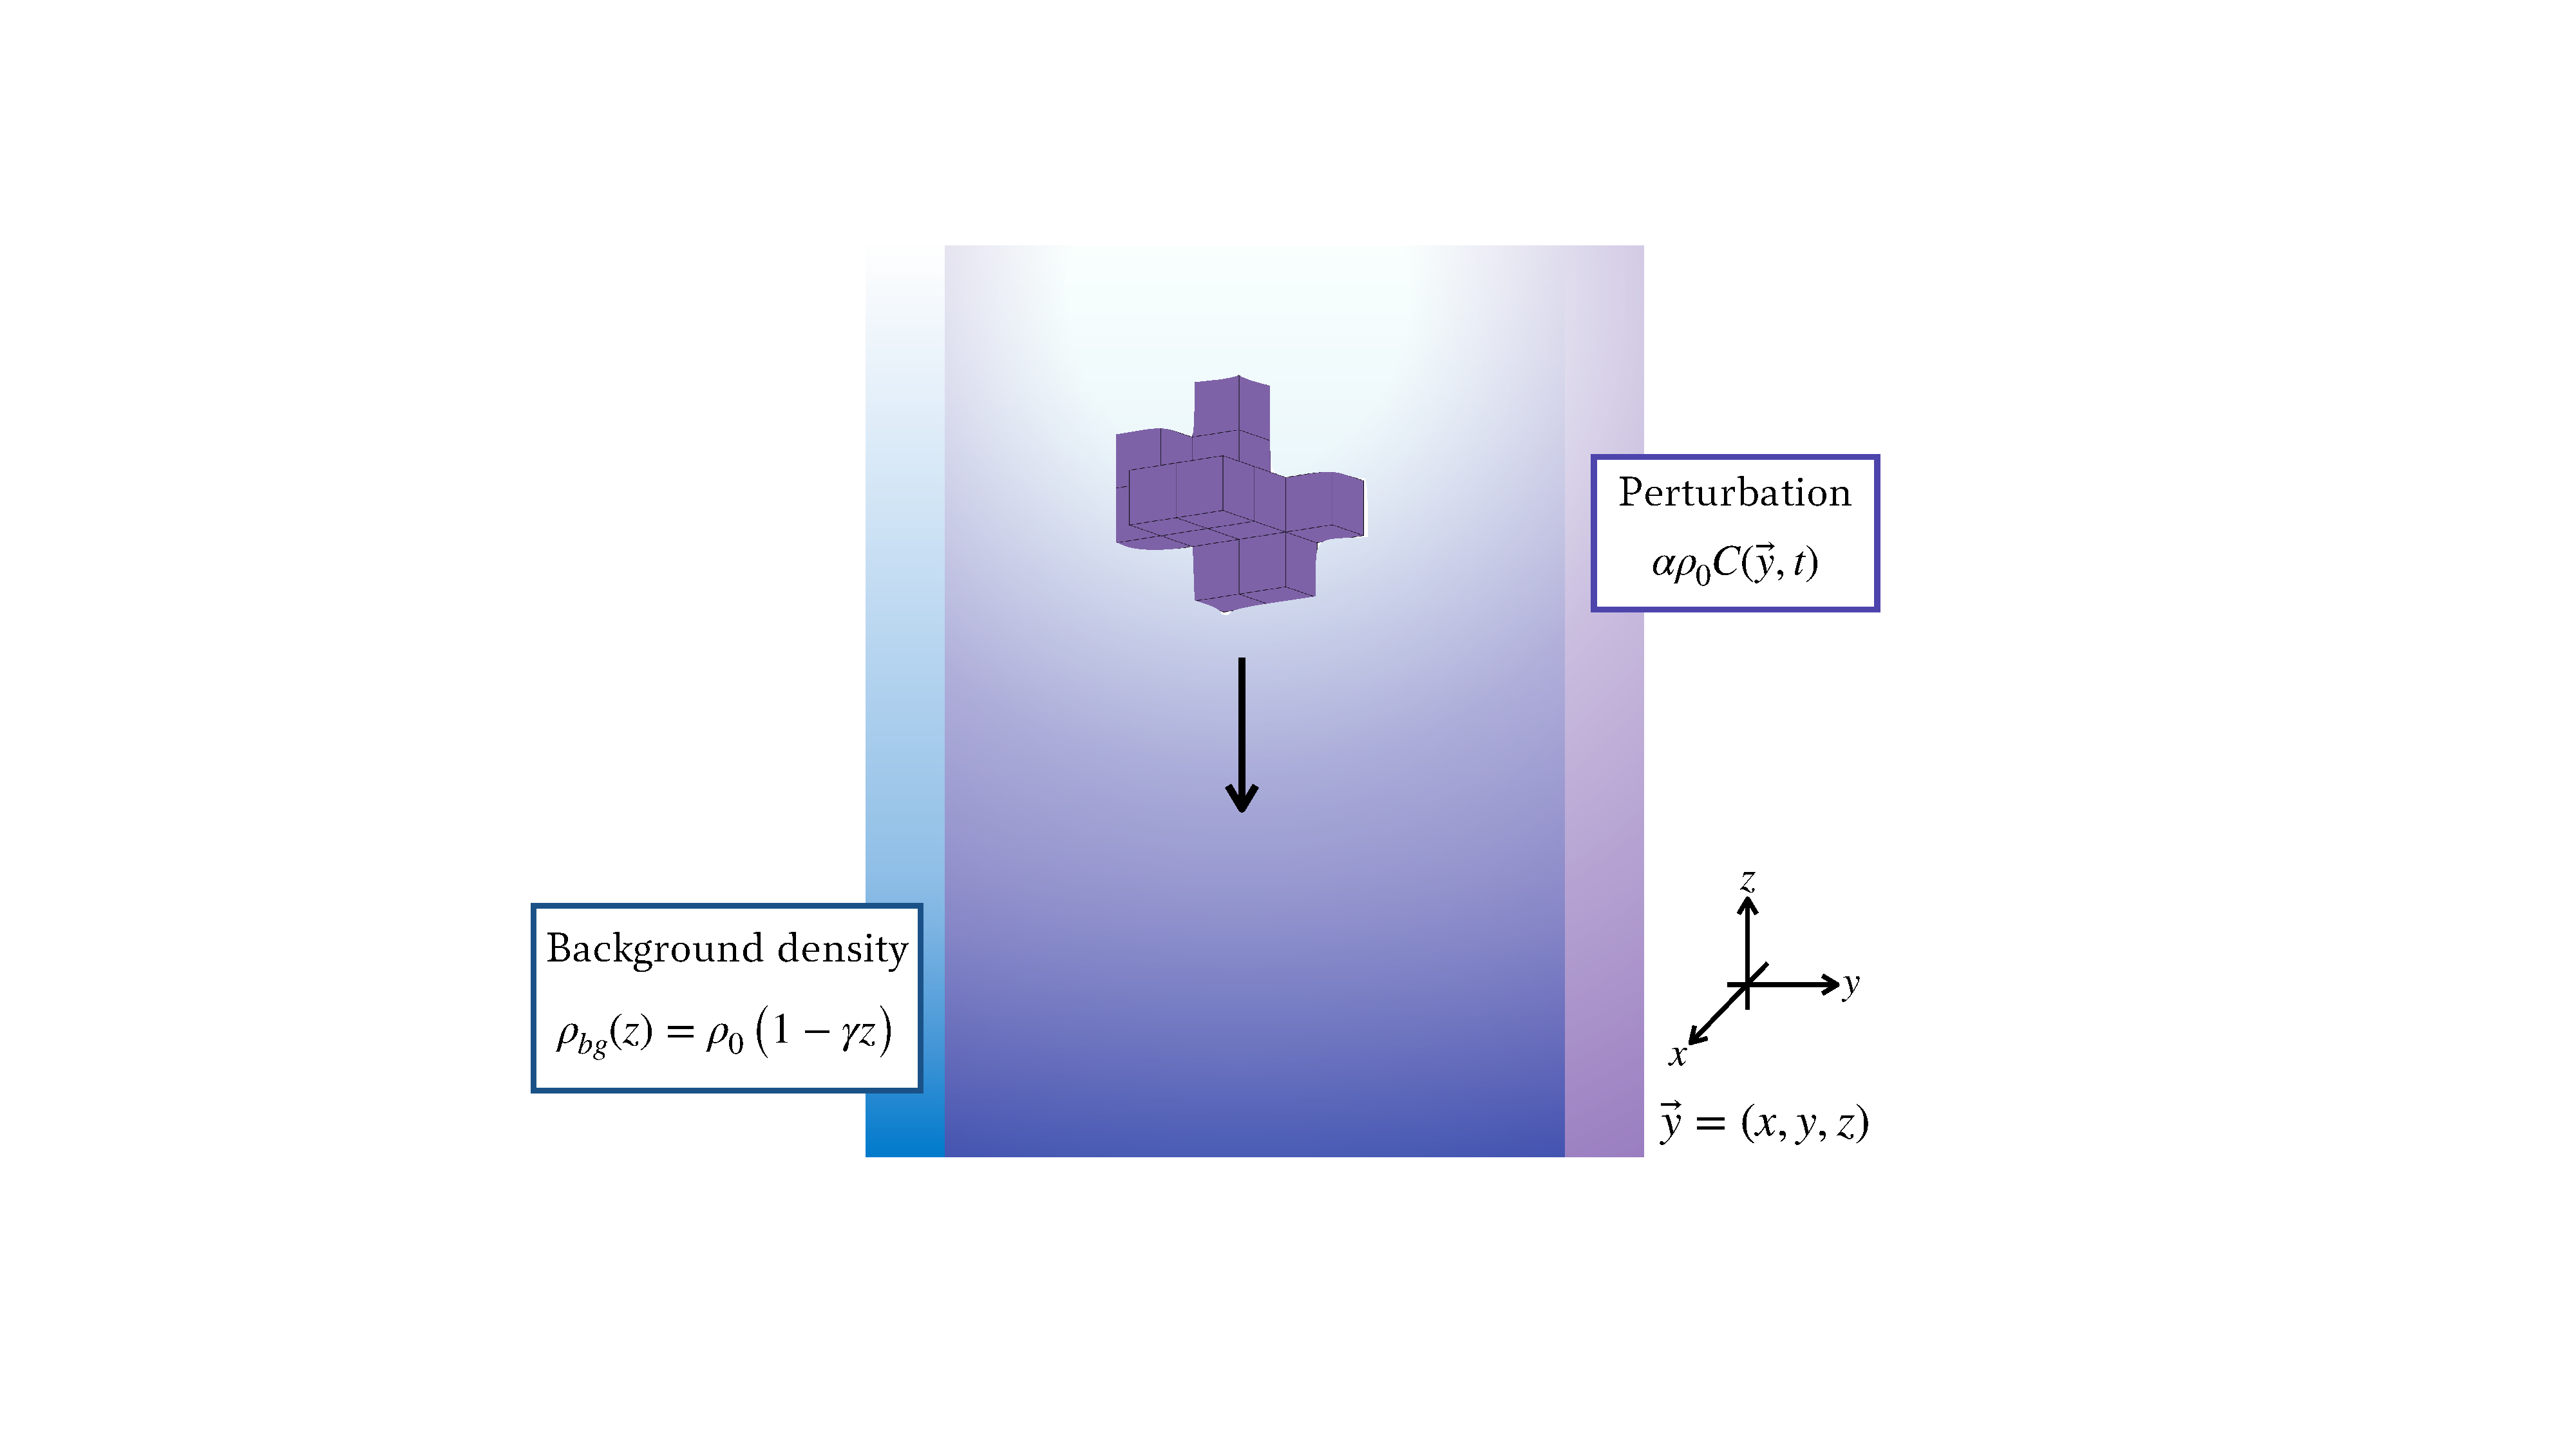
\includegraphics[scale=0.4]{./figures/fig_stratification_schematics}
	\caption{Description of fluid density stratification.}
	\label{fig_stratification_schematics}
	\end{center}
\end{figure}
To track the perturbation $C(\vec{y},t)$, we couple the advection-diffusion equation with the modified Stokes equations that we will describe in the next section. 
%------------------------------------------------------------------------------
\section{Governing Equations}
The non-constant density $\rho(\vec{y},t)$ plays a role as an external source of the fluid. This changes the momentum equation,
	Due to varying density, $\rho(\vec{y}, t)$, 
		 \begin{equation}
		\ \tilde{\mu}\nabla^2 \vec{u}(\vec{y})
		- \nabla P_d (\vec{y}) \ + \  
		 \rho_0 \alpha C(\vec{y},t) \vec{g} =0 , 
	\label{eq_extra_C}
	\end{equation}
	where $P_d$ is dynamic pressure, defined as
\begin{equation}
	P_d (\vec{y})
	 = P (\vec{y}) \ - \int \rho_{bg}(z) g   \textrm{d}z.
	\label{eq_Pd}
\end{equation}

In order to take the perturbation effect into account, we find the particular solution to the momentum equation (\ref{eq_extra_C}). Once we have one, simple addition to the homogenous solution would give us the entire solution due to the linearity of the system. 
\par
% \subsection{Particular solution to Stokes equations with the stratification}
%----------------------------------------------------------------------
To derive the particular solution, we consider the singularly forced Stokes problem \cite{pozrikidis_boundary_1992},
\begin{equation}
	\ \tilde{\mu} \nabla^2 \vec{u}(\vec{y})
	- \nabla P (\vec{y})
	+\vec{q} \ \delta \left(\vec{x} - \vec{y} \right) =0,
\label{eq_single_stokes}
\end{equation}
where $\vec{q}$ is an arbitrary constant vector, $\vec{y}$ is an arbitrary point in fluid domain, and $\delta$ is the three-dimensional delta function.
The problem (\ref{eq_single_stokes}) 
describes the effect coming from a single force applied at $\vec{x} = \vec{y}.$
The fundamental solutions to equation (\ref{eq_single_stokes}) with the continuity equation are
\begin{equation}
	\vec{u} (\vec{y}) = \ \frac{1}{8\pi \tilde{\mu}}  \bar{\bar{G \ }}(\vec{x}, \vec{y})
	\cdot  \vec{q}.
\label{eq_fund_u}
\end{equation}
\begin{equation}
	P (\vec{y}) = \ \frac{1}{4\pi }  
	\frac{\vec{x} - \vec{y}}{\| \vec{x} - \vec{y}\|^3}
	\cdot  \vec{q},
\label{eq_fund_p}
\end{equation}
where the kernel $\bar{\bar{G \ }}$ is called \textit{Stokeslet}, defined as 
\begin{equation}
	\bar{\bar{G}}( \vec{x}, \vec{y}) = 
	\frac{\bar{\bar{I \ }}}{||\vec{x}-\vec{y} ||} + \frac{(\vec{x}-\vec{y})(\vec{x}-\vec{y})^T}{||\vec{x}-\vec{y} ||^3}.
	% \label{eq_stokeslet_repeat}
\end{equation} 
This implies that the solutions (\ref{eq_fund_u}) and (\ref{eq_fund_p}) satisfy equation (\ref{eq_single_stokes}) as
\begin{equation}
	\ \tilde{\mu} \nabla^2 
	\biggl( \frac{1}{8\pi \tilde{\mu}}  \bar{\bar{G \ }}(\vec{x}, \vec{y})
	\cdot  \vec{q} \biggr)
	- \nabla \biggl(\ \frac{1}{4\pi }  
	\frac{\vec{x} - \vec{y}}{\| \vec{x} - \vec{y}\|^3}
	\cdot  \vec{q} \biggr)
	+ \vec{q} \ \delta \left(\vec{x} - \vec{y} \right)
	=0 .
\label{eq_single_stokes_sub}
\end{equation}
As we multiply by $\left( C(\vec{x}, t) \right)$ on both sides and integrate the entire equation over the domain, $V(\vec{x})$, we get
\begin{equation}
	\int_{V}
	\biggl[
	\ \tilde{\mu} \nabla^2 
	\biggl( \frac{1}{8\pi \tilde{\mu}}  \bar{\bar{G \ }}(\vec{x}, \vec{y})
	\cdot  \vec{q} \biggr)
	C(\vec{x}, t)
	-
	\nabla \biggl(\ \frac{1}{4\pi }  
	\frac{\vec{x} - \vec{y}}{\| \vec{x} - \vec{y}\|^3}
	\cdot  \vec{q} \biggr)
	C(\vec{x}, t)
	+ \vec{q} \ \delta \left(\vec{x} - \vec{y} \right)
	C(\vec{x}, t)
	\biggr]
	\ \textrm{d}V(\vec{x}) = 0 .
\label{eq_single_stokes_sub2}
\end{equation}
% Note that the right-hand side of equation (\ref{eq_single_stokes_sub2}) becomes $\vec{q} C(\vec{x},t)$ due to the integral of delta function.
Note that the operator $\nabla$ is linear and used with respect to $\vec{x}$, we are able to switch the order with the integral operator as following,
\begin{equation}
	\tilde{\mu} \ \nabla^2 
	\int_{V}
	\biggl( \frac{1}{8\pi \tilde{\mu}}  \bar{\bar{G \ }}(\vec{x}, \vec{y})
	\cdot  \vec{q} \biggr)
	C(\vec{x}, t)
	\ \textrm{d}V(\vec{x})
	-
	\nabla 
	\int_{V}
	\biggl(\ \frac{1}{4\pi }  
	\frac{\vec{x} - \vec{y}}{\| \vec{x} - \vec{y}\|^3}
	\cdot  \vec{q} \biggr)
	C(\vec{x}, t)
	\ \textrm{d}V(\vec{x})
	+\vec{q} C(\vec{x}, t) = 0 .
\label{eq_single_stokes_sub3}
\end{equation}
By choosing $\vec{q} = \rho_0 \alpha \vec{g}$, we can find
tha the particular solutions to our modified Stokes equations, (\ref{eq_extra_C}), as
\begin{equation}
	\vec{u} (\vec{y}) =
	 \frac{\rho_0 \alpha }{8\pi \tilde{\mu}}
	\int_{V}  \bar{\bar{G \ }}(\vec{x}, \vec{y})
	\cdot  C(\vec{x}, t) \vec{g} 
	\ \textrm{d}V(\vec{x}).
\label{eq_fund_soln_unit}
\end{equation}
\begin{equation}
	P(\vec{y}) = 
	\frac{\rho_0 \alpha }{4\pi }  
	\int_{V}
	\frac{\vec{x} - \vec{y}}{\| \vec{x} - \vec{y}\|^3}
	\cdot 
	C(\vec{x}, t) \vec{g} 
	\ \textrm{d}V(\vec{x}).
\label{eq_fund_soln_p}
\end{equation}
The entire velocity solution, thus, becomes
\begin{equation}
	 \vec{u} \left(\vec{y}, t \right) =
	 - \frac{1}{8 \pi \tilde{\mu}} \int_{S}  
		 \vec{f}(\vec{x}) 
		 \cdot \bar{\bar{G \ }} (\vec{x},\vec{y}) 
		 \ \textrm{d}S(\vec{x})
	+ \frac{ \rho_0 \alpha  }{8\pi \tilde{\mu}} \int_V  C \left(\vec{x},  t \right) \vec{g} \cdot 
	\bar{\bar{G \ }}(\vec{x}, \vec{y} ) 
	\ \text{d}V(\vec{x}).
\label{eq_vel_HP}
\end{equation}
As we see, the velocity at a point $\vec{u}$ is now depending on space and time. By coupling the solution (\ref{eq_vel_HP}) with the advection-diffusion equation, we can update the velocity field in time. 

%------------------------------------------------------------------
\subsection{Force balance}
\label{sec:force_balance}
\par
We also want to point out that we can no longer impose the velocity of the aggregate since it is not physically valid.
This implies that the velocity on the aggregate, equation (\ref{eq_solidbody}), that is
\begin{equation}
	\vec{u}_s (\vec{x}, t)  = \vec{U}_a + \vec{\Omega} \times (\vec{x}- \vec{x}_{cm}),
	\nonumber
\end{equation}
becomes unknown value. To be specific, we now need to solve for the translational and angular velocity, $\vec{U}_a$ and $\vec{\Omega}$, respectively, by prescribing the total body force and total torque. 
% We discuss the details of force balance in section \ref{sec:force_balance}.
% where $\vec{x}_{cm}$ is the center of mass of an aggregate. 
% We then have three unknowns for each face of the aggregate, $\vec{U}_a, \ \vec{\Omega}, $ and $\vec{f}$.
This should close the system since we have three vector equations to solve for all unknowns. 
As we mentioned, to close the system of equations, we prescribe the following total force, $\vec{F}_o$, and torque, $\vec{Q}_o $,
\begin{equation}
	\int_S \vec{f} (\vec{x}) \ \textrm{d}S = \vec{F}_o
\label{eq_Fo}
\end{equation}
and
\begin{equation}
	\int_S \vec{f}\times (\vec{x} - \vec{x}_{cm}) \ \textrm{d}S = \vec{Q}_o = \vec{0}.
\label{eq_Qo}
\end{equation}
 Note that the drag force is induced by the dynamic pressure $P_d$ defined in equation (\ref{eq_Pd}). This implies that 
\begin{equation}
	\vec{F}_o 
	 = - \int_S \left[ 
	 - \left( P -  \int \rho_{bg}(z) g \ \textrm{d}z \right) \bar{\bar{I \ }} 
	 + \tilde{\mu} \left( \nabla \vec{u} + (\nabla \vec{u})^{T} \right)
	 \right] \cdot \hat{n} \ \textrm{d}S (\vec{y}).
\label{eq_Fo_Pd}
\end{equation}
As we observe the stress tensor inside of equation (\ref{eq_Fo_Pd}), 
\begin{equation}
	\bar{\bar{\sigma \ }} = 
 -  P  \bar{\bar{I \ }} 
 + \tilde{\mu} \left( \nabla \vec{u} + (\nabla \vec{u})^{T} \right).
\end{equation}
Thus, the full body force, $\vec{F}$, can be found in the following net force balance equation at equilibrium,
\begin{equation}
	\vec{F}_o (t)
	  = - \vec{F}(t)
	  -  \int_S \left( 
	   \int \rho_{bg}(z) g \ \textrm{d}z 
	 \right) \bar{\bar{I \ }}  \cdot
	\hat{n} \ \textrm{d}S (\vec{y}).
\label{eq_Full_Force}
\end{equation}
The last term in equation (\ref{eq_Full_Force}) represents buoyancy acting toward the aggregate. 
This full body force, $\vec{F}$, can be also interpreted as the gravitational force acting on the aggregate,
\begin{equation}
	% \vec{F} = (\rho_a - \rho)V_a\vec{g}
	\vec{F}(t) = \rho_a(t) V_a \vec{g}, 
\end{equation}
where $\rho_a$  and $V_a$ are the aggregate density and volume, respectively. 
% In addition to equation (\ref{eq_vel_HP}), we may use equations (\ref{eq_Full_Force}) and (\ref{eq_total_Torque_dlp}) to solve for velocity $\vec{u}(\vec{x}_s)$ and the unknown density, $\vec{\psi} \in [0, 1]$, on the aggregate.
%------------------------------------------------------------------
% \subsection{Aggregate density}
Marine aggregates are typically very porous, yet their permeability is low. To take the porosity, denoted as $\phi \in [0,1]$, into account, we define the density of an aggregate as 
\begin{equation}
	\rho_a (t) = \phi \rho_{f}(t) + (1-\phi) \rho_{s},
	\label{eq_rho_a}
\end{equation}
where $\rho_{f}$ and $\rho_s$ are the liquid and solid portion of the entire aggregate density, respectively. To obtain the liquid portion of the aggregate density, we take an average of fluid density where the aggregate locates $\rho_{f},$
\begin{equation}
	\rho_{f}(t) = \frac{1}{V_a}\int_{V_a} \rho(\vec{x}, t) \  \textrm{d}V(\vec{x}))
\end{equation}
For now, we consider the solid part of the aggregate density as $\rho_s \approx 1400 $kg$/$m$^3.$ 
We also set the porosity about $95\%$, or $\phi = 0.95$.

% I don't think the following belongs here:

%--------------------------------------------------
\subsection{Advection-Diffusion equation}
Since the perturbation $C(\vec{x}, t)$ is time dependent, we couple the Stokes equations with the advection-diffusion equation to update $C(\vec{x}, t)$ in time. To take the background density into account, what we should update is the entire fluid density,
\begin{equation}
	\frac{\partial \rho(\vec{y},t)}{\partial t}
	+ \vec{u}(\vec{y}) \cdot \nabla \rho(\vec{y},t)
	 = D \nabla^2 \rho(\vec{y},t),
\label{eq_AD_rho}
\end{equation}
where $D$ is diffusion coefficient.
For salinity of seawater, we find the diffusion coefficient, $D_{salt} = 2 \times 10^{-9}  (\text{m}^2\text{/s})$ from \text{\it Wollast and Garrels (1971)} \cite{wollast_diffusion_1971}. In addition, we recall the aggregate's settling speed ($U_s$), its maximum radius ($R_a$),
\begin{align}
	\text{Pe} 
	= \frac{U_s R_a }{D_{salt}} 
	\approx \frac{3.8 \times 10^{-4}(\text{m/s}) \times \left(5 \times 10^{-5} \right) (\text{m})}{2 \times 10^{-9} (\text{m}^2\text{/s})} = 9.5
\end{align}
\par 
For the thermal diffusivity, $D_{heat}$, we cosider the value referred by {\it Nayar et. al (2016)} \cite{nayar_thermophysical_2016} and {\it Sharqawy et. al (2010)} \cite{sharqawy_thermophysical_2010},
\begin{align}
	\text{Pe} 
	= \frac{U_s R_a }{D_{heat}} 
	\approx \frac{3.8 \times 10^{-4}(\text{m/s}) \times \left(5 \times 10^{-5} \right) (\text{m})}{1.5 \times 10^{-7} (\text{m}^2\text{/s})} \approx 10^{-2}.
\end{align} 
Since the fluid is density is evolving only in the gravitational direction, $z-$direction, we can simplify the re-write the equation (\ref{eq_AD_rho}) in terms of $C(z,t)$, 
\begin{equation}
	\frac{\partial C(z,t)}{\partial t}
	+ \vec{u}(\vec{y}) \cdot \nabla C(z,t)
	 = D \nabla^2 C(z,t)
	 - \frac{\gamma}{\alpha}\vec{u}(\vec{y})  \cdot \hat{k}.
\label{eq_AD_C}
\end{equation}
We track the perturbation $C(z,t)$ for every time step by solving the equation (\ref{eq_AD_C}).
%------------------------------------------------------------------
\section{Non-dimensionalization}
To facilitate further analysis, we non-dimensionalize our new equations. We mainly use the same parameters we introduced in section \ref{section3}, equations (\ref{eq_nonD}), in addition to the following dimensionless parameters:
\begin{equation}
	C= C_{max} C'
\hspace{7mm}
\rho = \frac{\tilde{\mu}  }{{U_s} R_a}  \rho', 
\end{equation}
In this chapter, the Stokes settling speed $U_s$, defined in equation (\ref{eq_U_s}), becomes
\[
U_s = \frac{g  L^2}{\tilde{\mu}}(\rho_s - \rho_0)(1-\phi),
\] 
since we consider the porosity of an aggregate as (\ref{eq_rho_a}).
% Note that the Reynolds number is approximately 0.03.
 % Here $\rho_a$ is the density of aggregate.
For the scale of the perturbation, $C$, we introduce the maximum density difference of the background density profile in the fluid domain at initial time, i.e., 
\[
C_{max} = 
\left|
\max_{(x,y,z) \in V} \left(\rho_{bg}(z)  \right)
\ - \min_{(x,y,z) \in V} \left(\rho_{bg}(z)  \right) \right|.
 % \left| \tilde{S}(z_\text{top}, \ 0 )
 % - \tilde{S} \left( z_\text{bottom}, \ 0 \right) \right|. 
\] 
As we want to see the settling of an aggregate throughout the fluid having density gradient, we decided to have 1\% density difference between top and bottom layers of fluid domain.
%  {\color{red}NEED NUMBER WITH UNIT AND A REFERENCE!}
\par
We first derived the dimensionless modified Stokes momentum equation,
\begin{equation}
	{\nabla'}^2  \vec{u}'(\vec{y})
	= \nabla {P_d}'(\vec{y}) \ - \  
	\frac{\rho_0}{(\rho_s - \rho_0)(1-\phi)} \alpha C_{max} C'\left(\vec{y},t \right)   \hat{k},
\label{eq_extra_C_nonD}
\end{equation}
along with the velocity field
%  on the aggregate boundary surface $\vec{y}' = \vec{x}'_s$, using 
 \begin{align}
		\vec{u}'(\vec{y})
			  & =- \frac{1}{8 \pi} \int_{S'}  
			 \vec{f'}(\vec{x}) 
			 \cdot \bar{\bar{G' \ }} (\vec{x},\vec{y}) 
			 \ \textrm{d}S'(\vec{x})
			 \nonumber \\
& -\frac{ \alpha C_{max}}{8\pi } \frac{\rho_0}{(\rho_s - \rho_0)(1-\phi)} 
\int_{V'} C' \left(\vec{x},  t \right) \hat{k} \cdot 
\bar{\bar{G'  }}(\vec{x}, \vec{y} ) 
\ \text{d}V'(\vec{x})
  \label{eq_vel_all_onS_nonD}
 \end{align}
where $S$ is the aggregate surface. 
Moreoever, the force balance equation (\ref{eq_Full_Force}) becomes
\begin{align*}
	 \vec{F'}_o(t)
	 & =
	   %\text{[Body force] + [Buoyancy force]}
	  %= 
	  \frac{1}{\tilde{\mu} U_s L} 
	  \left(
	-   \rho_a V_a g \hat{k}
	  +
	   \int_{S} \left( 
	   \int \rho_{bg}(z) g \ \textrm{d}z 
	   \right) \bar{\bar{I \ }}  \cdot
	  \hat{n} \ \textrm{d}S (\vec{x})
	\right).
	% \\
	% &=  \frac{g}{\tilde{\mu} U_s L}\frac{\tilde{\mu}  L^3 }{U_s L}
	% \left( 
	% - \rho_a' V_a' \hat{k}
	% + \int_{S'} \left( 
	%    \int  {\rho}_{bg}'(z) \ \textrm{d}z' 
	%  \right) \bar{\bar{I \ }}  \cdot
	% \hat{n} \ \textrm{d}S' (\vec{x})
	% \right)
	% \\
	% &=  \frac{gL}{U_s^2 }
	% \left( 
	% - \rho_a' V_a' \hat{k}
	% + \int_{S'} \left( 
	%    \int  {\rho}_{bg}'(z) \ \textrm{d}z' 
	%  \right) \bar{\bar{I \ }}  \cdot
	% \hat{n} \ \textrm{d}S' (\vec{x})
	% \right).
\label{eq_Full_Force_nonD}
\end{align*}
% Note that the volume of aggregate $V_a$ is $8$NC  in our numerics, where NC is the number of cubes to form an aggregate. The factor 8 comes from the side length of each cube that is 2. By letting the characteristic length scale that is the maximum radius, in numerics denoted by $R_m$, we find dimensionless tull body force $\vec{F}'$ as
% \begin{equation}
% 	\vec{F'}
% 	 = -  \frac{\rho_a}{\rho_0}\frac{8 \textrm{NC}}{{R_m}^3}\hat{k}
% \label{eq_Full_bodyForce_nonD}
% \end{equation}

% The velocity field changes in time since the perturbation $C$ varies in timeX
\par
Lastly, the advection-diffusion equation becomes, 
	\begin{equation}
	\frac{\partial C'(\vec{x},t)}{\partial t'}
	+ \vec{u}'(\vec{x}) \cdot \nabla' C'(\vec{x},t)
	 = \frac{1}{\textrm{Pe}} {\nabla'}^2 C'(\vec{x},t)
	 -\frac{\gamma R_a}{ \alpha C_{max}} \vec{u}' \cdot \hat{k},
	\label{eq_AD_nonD}
	\end{equation}
using the velocity field, equation (\ref{eq_vel_all_onS_nonD}), for the advection term.
For the rest of this chapter, we drop the prime for simplicity and use only dimensionless forms. 
\begin{comment}
For more efficient numerical simulation, we use moving frame of reference to solve the advection-diffusion equation, by letting the velocity in the moving frame, $\vec{u}_m $, as
\[
\vec{u}_m = \vec{u} - \vec{U}_a,
\]
where $\vec{U}_a$ is translational velocity.
 To proceed, we may change the variables from the lab fram to the moving frame as following:
\[
\vec{x}_m = \vec{x} -\vec{U}_a t, \ \ \ \ \ 
t_m = t.
\]
Using chain rules, equation (\ref{eq_AD_nonD}) then becomes 
\begin{equation}
	\left( \frac{\partial}{\partial t}  \frac{\partial t}{\partial t_m}
	+ \frac{\partial}{\partial \vec{x}_m}  \frac{\partial \vec{x}_m}{\partial t_m} \right)
	C(\vec{x}_m, t_m)
	+ \left( \vec{u}_m(\vec{x}_m) + \vec{U}_a \right) \cdot \nabla C(\vec{x}_m , t_m)
	 = \frac{1}{\textrm{Pe}} {\nabla}^2 C(\vec{x}_m, t_m)
	 -\frac{\gamma L}{ \alpha C_{max}} \left( \vec{u}_m(\vec{x}_m) + \vec{U}_a \right) \cdot \hat{k}.
	 \nonumber
	% \label{eq_AD_nonD_moving}
\end{equation}
Since $\partial x_m / \partial t_m = -\vec{U}_a$, we can simplify few terms. After we go back to typical coordinate notation, we obtain
	\begin{equation}
 \frac{\partial C(\vec{x}, t)}{\partial t}  
		+ \vec{u}_m(\vec{x})  \cdot \nabla C(\vec{x},t)
		 = \frac{1}{\textrm{Pe}} {\nabla}^2 C(\vec{x},t)
		 -\frac{\gamma L}{ \alpha C_{max}} \left( \vec{u}_m(\vec{x}) + \vec{U}_a \right) \cdot \hat{k}.
		\label{eq_AD_nonD_moving}
	\end{equation}
%
\end{comment}
%Rotation==============================================
\section{Rotation}
{\color{blue}QUESTION: MAYBE I SHOULD MOVE THIS SECTION TO NUMERICAL METHODS?}
\begin{comment}
The big picture of applying rotation to our simulation is the following:
\begin{itemize}
	\item With the obtained angular velocity, $\Omega$, from the previous time step
	\item Compute the rotation matrix, $\mathcal{R}$ 
	\item Rotate the aggregate position using updated $\mathcal{Q}$
	\item Solve for stress, $\vec{f}$
	\item Evalutate the velocity field 
	\item Update the perturbation
\end{itemize}

To explain this mechanism, we need to be careful about the three different types of points in the entire system: $\vec{x}, \vec{y}, $ and $\vec{x}_s$. 
First, $\vec{x}$ is the points of the entire fluid domain  $V$, i.e., $\vec{x} \in V$. This may different from the points that we want to obtain the velocity, in which we denote as $\vec{y}$. For our full simulation, we most likely have $\vec{x} = \vec{y}$.
% although this does not have to be necessary.
In addition, $\vec{x}_s$ is the point on the surface of the aggregate, i.e., $S$ is the aggregate boundary. 
\\
In this rotation section, we assume $\vec{x}=\vec{y}$ since we would like to obtain the velocity field everywhere in the fluid domain. We need to distinguish $\vec{x}$ and $\vec{x}_s$ carefully. 
Note that for both grid systems, the center of the domain is fixed as the center of mass of the aggregates, $\vec{x}_{cm}.$
See Figure \ref{fig_schematics} to understand the notations. For simplicity, we draw the schematics in two-dimensional space.
    \begin{figure}[ht]
    	\begin{center}
    		\vspace{0.5cm}
    		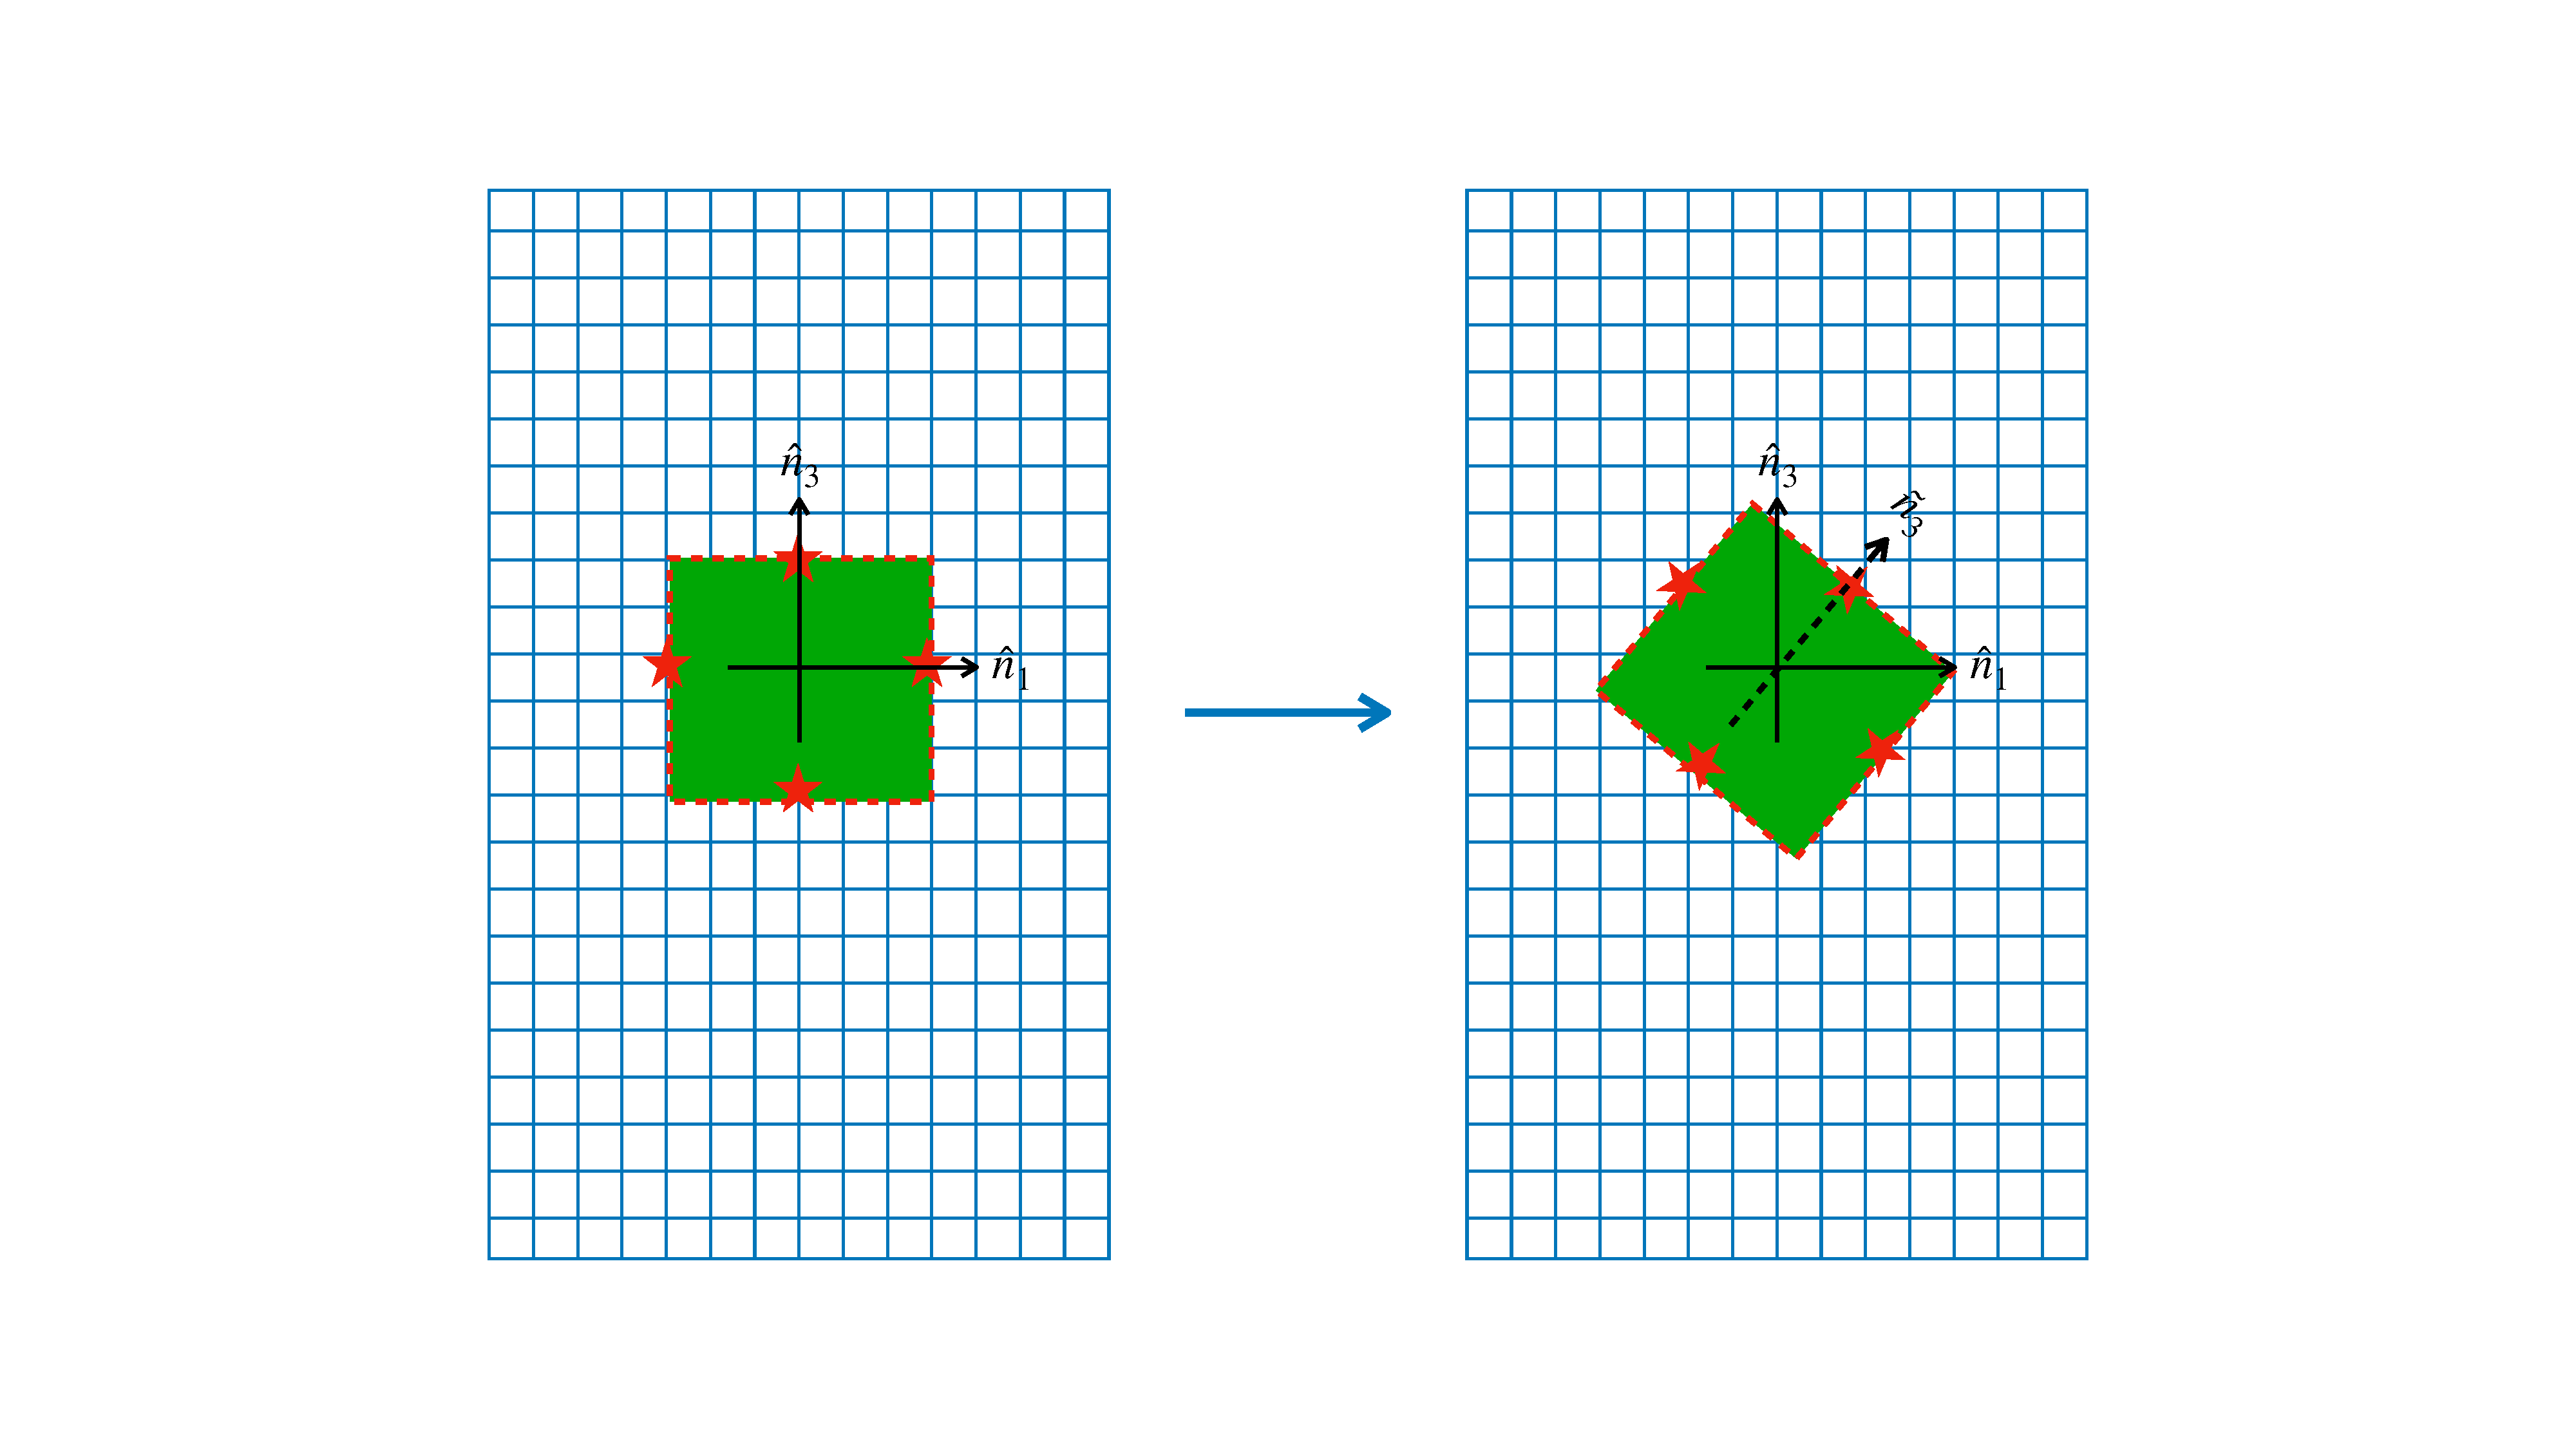
\includegraphics[scale=0.25]{./figures/fig_schematics}
		
    	\caption{Schematics of the rotation of aggregate.}
    	\label{fig_schematics}
    \end{center}
    \end{figure}
The points $\vec{y}$ are the blue grid in Figure \ref{fig_schematics} and the discretized version of $\vec{x}_s \in S$ are, in particular, the center of each square face. These are shown with red stars. We let the left-side plot in Figure \ref{fig_schematics} is the grid at time $t_n$ and the one after arrow shows the grid at time $t_n + \Delta t$.
\par
(Within a time step) When we solve for stress, $\vec{f}(\vec{x}_s)$, we also find aggregate's translational and angular velocities. 
\end{comment}
\\
In order to have more realistic simulations, we allow our aggregate model to rotate while they settle.
We here focus on the angular velocity, $\vec{\Omega} = \Delta \theta / \Delta t$, which tells us how much the aggregate rotates ($\theta)$ in one time step, $\Delta t$. 
\begin{figure}[ht]
	\begin{center}
		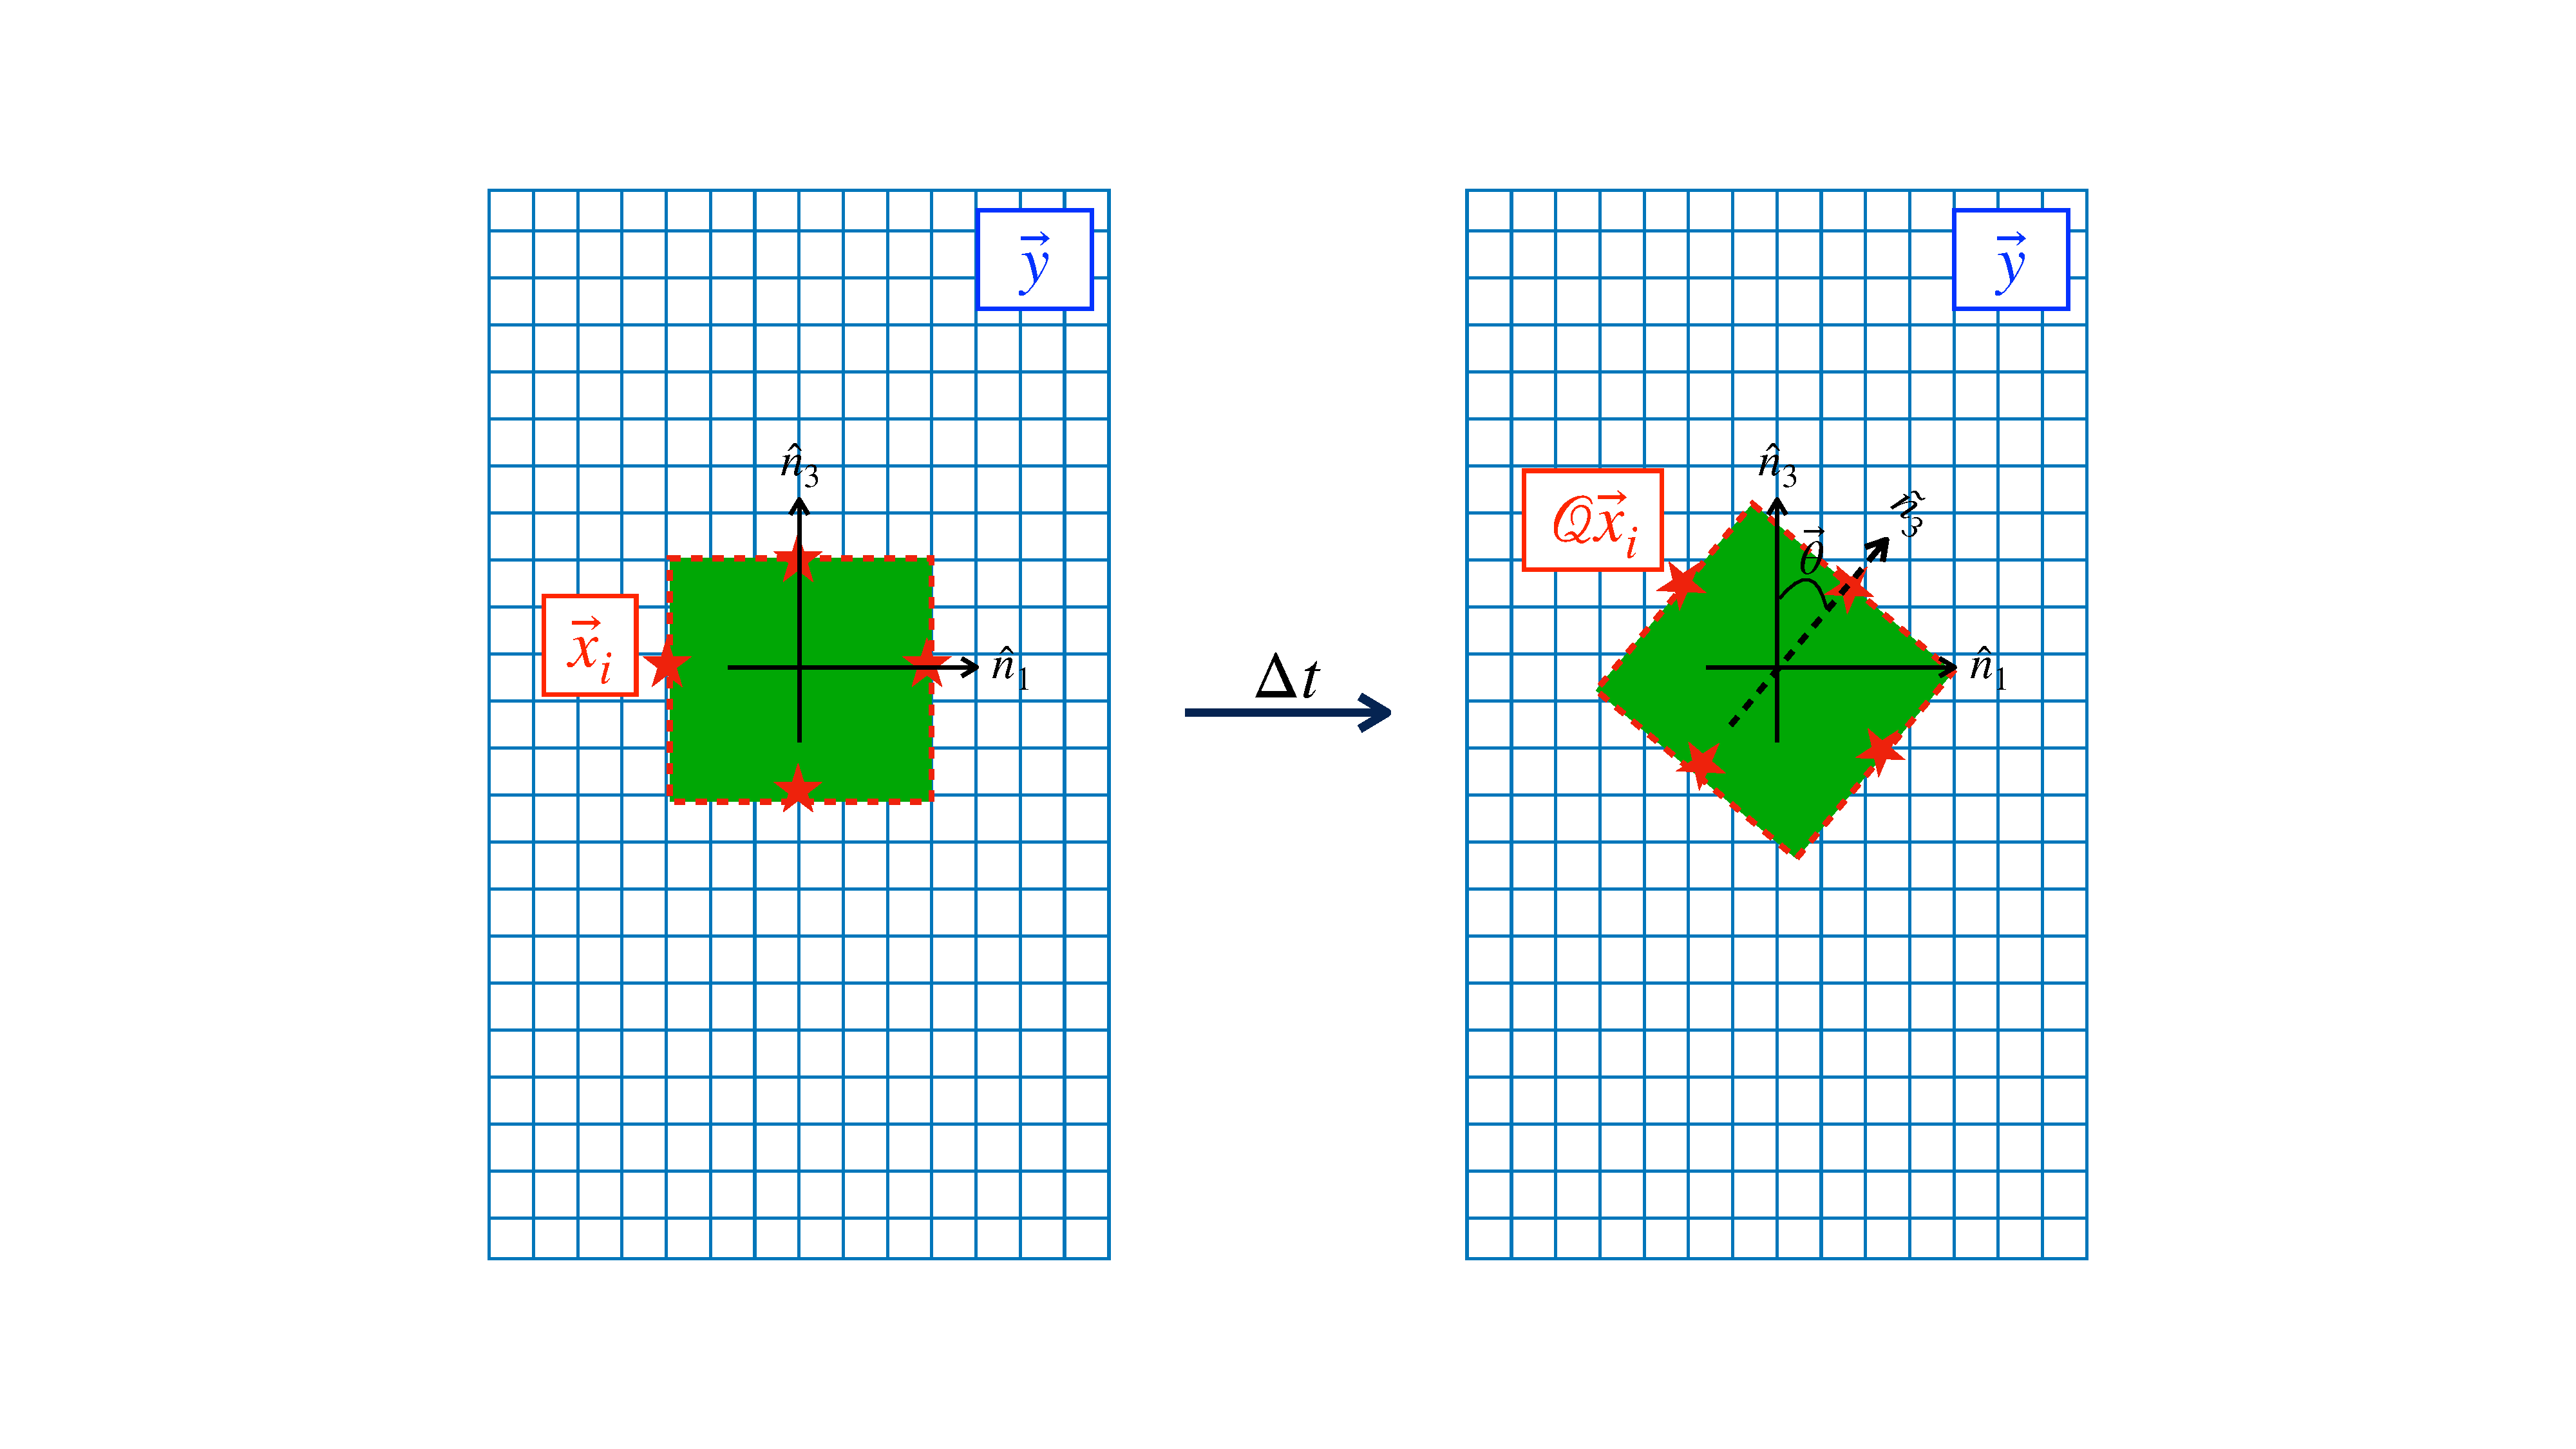
\includegraphics[scale=0.25]{./figures/fig_rotation_schematics.pdf}
	\caption{Schematics of the rotation of an aggregatem. Blue grid is the fluid domain and green rectangle represents an aggregate. Red stars show points on the aggregate.}
	\label{fig_rotation_schematics}
\end{center}
\end{figure}
This information lives in the orientation matrix, $\mathcal{Q}(t)$. We can update our aggregate position from $\vec{x}$ to $\vec{x}_{\mathcal{R}}$ using
\[
\vec{x}_{\mathcal{R}}(t) = \mathcal{Q}(t) \vec{x}.
\]
Note that $\mathcal{Q}(0) = \bar{\bar{I}}$ (identity matrix) at initial time. After we move forward one time step, we may update this orientation matrix as 
\begin{equation}
	\mathcal{Q}(t + \Delta t) = \mathcal{R} \mathcal{Q}(t),
\end{equation} 
where $\mathcal{R}$ is the rotation matrix. 
\par
Assume that we obtain the angular velocity, $\vec{\Omega}$ from a time step. (Initially, it is zero vector). With this, we can find the three-dimensional change of angular position vector, $ \vec{\Omega} \Delta t = \left( \Delta \theta_1, \ \Delta \theta_2, \ \Delta \theta_3 \right) \equiv \Delta \vec{\theta}$.
The matrix $\mathcal{A}$ is then defined as 
\begin{equation}
	\mathcal{A}
	=\begin{bmatrix}
	 0 & - \Delta \theta_3 & \Delta \theta_2  \\
	 \Delta \theta_3 & 0  & -\Delta \theta_1  \\
	 - \Delta \theta_2 & \Delta \theta_1 & 0  \\
	\end{bmatrix},
	\label{eq_rotation_mx}
\end{equation}
From here, we have the rotation matrix $\mathcal{R} = e^{\mathcal{A}}.$
We can compute the matrix exponential $e^{\mathcal{A}}$ using Rodrigues' formula,
\begin{equation}
	\mathcal{R} = 
e^{\mathcal{A}} 
 = \bar{\bar{I \ }} 
 + \frac{\sin(\phi)}{\phi} \mathcal{A}
 + \frac{1-\cos(\phi)}{\phi^2} \mathcal{A}^2,
\label{eq_R_eA}
\end{equation} 
where $\phi = \|\Delta \vec{\theta}\|_2$.
With this $\mathcal{R}$ and orientation matrix $\mathcal{Q}$, we are ready to update fluid grid.


	
\subsection{Linear system in a rotated coordinate}
We first solve for the stress at the center of each square face of an aggregate, $\vec{y} = \vec{x}_i$, 
using the same formula as equation (\ref{eq_vel_all_onS_nonD}),
\begin{equation}
	\vec{u} \left(\vec{x}_i \right) 
		  = -\int_{S}  
		 \vec{f}(\vec{x}) 
		 \cdot \bar{\bar{G \ }} (\vec{x}, \vec{x}_i) 
		 \ \textrm{d}S 
		 - \frac{ \alpha C_{max}}{8\pi } \frac{\rho_0}{(\rho_s - \rho_0)(1-\phi)}
		 \int_V  C \left(\vec{x} ,t \right) \hat{k} \cdot
		 \bar{\bar{G \ }}(\vec{x}, \vec{x}_i)
		 \ \text{d}V,
		 \nonumber
\end{equation}
As we allow rotation, we can express the above equation as
\begin{align}
	\vec{u} \left(\mathcal{Q} \vec{x}_i \right) 
		  = & - \frac{1}{8 \pi} \int_{S}  
		 \vec{f}(\mathcal{Q} \vec{x}) 
		 \cdot \bar{\bar{G \ }} (\mathcal{Q} \vec{x},\mathcal{Q}\vec{x}_i) 
		 \ \textrm{d}S
		 \nonumber \\
		 & - \frac{ \alpha C_{max}}{8\pi } \frac{\rho_0}{(\rho_s - \rho_0)(1-\phi)}
		 \int_V  C \left(\vec{x} ,t \right) \hat{k} \cdot
		 \bar{\bar{G \ }}(\vec{x}, \mathcal{Q} \vec{x}_i)
		 \ \text{d}V.
	\label{eq_slp_On_rotate}
\end{align}
Since the rotation matrix $Q$ is constant and it is normalized, it is valid to say that
\[
 \bar{\bar{G \ }} (\mathcal{Q} \vec{x},\mathcal{Q}\vec{x}_i) 
	 = \bar{\bar{G}}( \vec{x}, \vec{x}_i).
\]
% Precisely, we use the following form in Matlab program:
% \begin{equation}
% 	\vec{u} \left(\mathcal{Q} \vec{x}_i\right) 
% 		  + \frac{1}{8 \pi} \int_{S}  
% 		 \vec{f}(\mathcal{Q} \vec{x}_i) 
% 		 \cdot \bar{\bar{G \ }} (\vec{x},\vec{x}_i) 
% 		 \ \textrm{d}S(\vec{x}_s) 
% 		 =
% 		 - \frac{ \alpha C_{max}}{8\pi } \frac{\rho_0}{(\rho_s - \rho_0)(1-\phi)}
% 		 \int_V  C \left(\vec{x} ,t \right) \hat{k} \cdot
% 		 \bar{\bar{G \ }}(\vec{x}, \mathcal{Q} \vec{x}_i)
% 		 \ \text{d}V(\vec{x}).
% 	\label{eq_slp_stress_aggR}
% \end{equation}
We now solve for has unknowns, including the translational and angular velocities,
in a rotated coordinate system $\mathcal{Q} \vec{x}_i $.
Note that the stress values we obtain here 
are located in the same one as the rotated positions.  
To complete the linear system to solve for stress, translational, and angular velocities, we temporarily map fluid domain grid into the same coordinate system as the boundary inegral term.
We can simply muptipliy by $\mathcal{Q}^{-1} = \mathcal{Q}^{T}$ as 
\begin{align}
	\vec{u} \left(\mathcal{Q} \vec{x}_i \right) 
		  & + \frac{1}{8 \pi} \int_{S}  
		 \vec{f}(\mathcal{Q} \vec{x}) 
		 \cdot \bar{\bar{G \ }} (\mathcal{Q} \vec{x},\mathcal{Q}\vec{x}_i) 
		 \ \textrm{d}S
		 \nonumber \\ & =
		 \mathcal{Q}^{-1}
		 \left[
		 - \frac{ \alpha C_{max}}{8\pi } \frac{\rho_0}{(\rho_s - \rho_0)(1-\phi)}
		 \int_V  C \left(\vec{x} ,t \right) \hat{k} \cdot
		 \bar{\bar{G \ }}(\vec{x}, \mathcal{Q} \vec{x}_i)
		 \ \text{d}V
		 \right].
	\label{eq_slp_vol_R}
\end{align}
For the other force equations as well, we implement the following
\begin{equation}
	\int_{S} \vec{f}(\vec{x}) \  \text{d}S(\vec{x})
	= \mathcal{Q}^{-1} \vec{F}_o
	 \label{eq_drag_code}
	 \end{equation} 
	 \begin{equation}
		 \int_S \vec{f} (\vec{x})  \times (\vec{x} - \vec{x}_{cm}) 
		 \ \textrm{d}S(\vec{x}) 
		 = \vec{0}.
	 \label{eq_torque_code}
	 \end{equation}
Once we solve the linear system ,
 we may put the values on the fluid grid back into the Cartesian coordinate system.
% We need to rotate them using
% \[
% \vec{f}(\vec{x}_s) = \mathcal{Q} \vec{f}(\vec{x}).	
% \]
% \[
% \vec{U}_a (\vec{x}_s) = \mathcal{Q} \vec{U}_a (\vec{x}).	
% \]
% \[
% \vec{\Omega}(\vec{x}_s) = \mathcal{Q} \vec{\Omega}(\vec{x}).	
% \]
% The validation of stress is in section (\ref{validation_rot}).
\subsection{Velocity compuation}
Once we solve for the stress, we are supposed to use the same 
equation (\ref{eq_vel_all_onS_nonD}) 
to solve for velocity in the fluid grid which stays in the Cartesian coordinates.
Although the volume integral term can stay as it is,  
the boundary integral needs some special treatment
since it has two mixed coordinates systems.
We particularly pay more attention to the Stokeslet,
\[
	\bar{\bar{G \ }} (\mathcal{Q}\vec{x},\vec{y}) 
	= 
	\frac{\bar{\bar{I \ }}}{||\mathcal{Q}\vec{x}-\vec{y} ||} 
	+ \frac{(\mathcal{Q}\vec{x}-\vec{y})(\mathcal{Q}\vec{x}-\vec{y})^T}{||\mathcal{Q}\vec{x}-\vec{y} ||^3}, 	 
\]
where $\mathcal{Q}\vec{x}$ is in the aggregate rotated grid. Since we cannot compute the boundary integral of the Stokeslet when $\mathcal{Q}\vec{x}$ and $\vec{y}$ are not in the same coordinate system, we need to express $\vec{y}$ using another vector $\vec{v}$ that is in the rotated grid such that 
\[
	\mathcal{Q}\vec{x} - \vec{y} = \vec{x} - \vec{v},
	% \mathcal{Q}\vec{x}-\vec{v} = \vec{x} - \vec{y},
\]
or equivalently,
\[
	\vec{v} = \left(   \bar{\bar{I}} - \mathcal{Q} \right) \vec{x}  + \vec{y}.
\]
% {\color{blue} Need to type below figure.}
% \begin{figure}[h]
% 	\begin{center}
% 		\includegraphics[scale=0.45]{./figures/fig_vel_y_map}		
% 		\caption{Mapping for $\vec{y}$ grid.}
% 		\label{fig_vel_y_map}
% \end{center}
% \end{figure}

After we solve for the velocity field of the fluid domain, we rotate the velocity field back to the original coordinate by multiplying by inverse of $\mathcal{Q}$ for the concentration update. 
%---------------Numerics--------------------------------------
\section{Numerical methods}
%------------------------------------------------------------------
*We drop the prime for all dimensionless equations. 
\\
In this section, we explain the details of numerical methods. We first consider the background fluid density that is a part of the drag computation. We derive the simplest form to implement in codes. We then discuss the homogeneous velocity field. We compare two boundary integral equations since it was not straightforward to choose one. Lastly, we present the method to compute the non-homogeneous solution which is a volume integral of the perturbation $C(\vec{x},t)$. Due to the high computational cost, we use the fast multipole method (FMM). We give a brief introduction of the FMM and framework for Stokes kernel.
 \subsection{Background fluid density}
In this section, we explain how to compute the (dimensional) buoyancy term in equation, that is
\begin{equation}
	\rho_{by} =
	 \int_{S} \left( 
	   \int  {\rho_{bg}} (z) g \ \textrm{d}z
	 \right) \bar{\bar{I \ }}  \cdot
	\hat{n} \ \textrm{d}S (\vec{x}).
\label{eq_buoyancy2}
\end{equation}
We consider a single cube case for simplicity, i.e., $Nf = 6$. We can simply extend it to multiple cubes in the same manner. The discretized version of integral (\ref{eq_buoyancy2}) is 
\begin{equation}
	\sum_{i=1}^{Nf}
	 L^3 \int_{S^i} \left( 
	   \int  {\rho_{bg}} (z) g  \ \textrm{d}z 
	 \right) \bar{\bar{I \ }}  \cdot
	\hat{n}_i \ \textrm{d}S^i (\vec{x}),
\label{eq_buoyancy_discrete2}
\end{equation}
where $i$ represents the index of square faces (not a power). Note that we muptiply by $L^3$ to keep the dimensionality. Depending on the orientation of each square face, the integral domain or axis of $S^n$ is different. For example, let $S^1$ be the first square with the normal $\hat{n}_1 = (1,0,0)$. Then 
\begin{equation}
	L^3 
	 \int_{S^1}
	 \left( 
	   \int  {\rho_{bg}} (z) g \ \textrm{d}z 
	 \right) \bar{\bar{I \ }}  \cdot
	\hat{n}_1 \ \textrm{d}S^1 (\vec{x})
	= L^3  \int_{-1}^{1} \int_{-1}^{1}
	\left( 
  	 \int  {\rho_{bg}} (z) g \ \textrm{d}z 
 	\right) \bar{\bar{I \ }}  \cdot
 	\hat{n}_1 \ 
	\textrm{d}y  \textrm{d}z 
\label{eq_buoyancy_S1_2}
\end{equation}
Since the background function $\rho_{bg}$ is a function of $z$ only,intuitively, we see that the value (\ref{eq_buoyancy_S1_2}) and the one with the normal $\hat{n}_6 = -\hat{n}_1 = (-1,0,0)$ has the same magnitude but in the opposite direction. This means that when we add the integrals on $S^1$ and $S^6$, we get zero. We can also prove this with simple arithmetics. 
\par
We first write the inner integral explicitly using
\[
L^3 \int  {\rho_{bg}} (z)g  \ \textrm{d}z 
 =  L^3 \left( \rho_0 \int  1+\gamma  z \right) g \ \textrm{d}z 
=L^3 \rho_0 \left(  z + \frac{\gamma}{2}z^2 + c \right) g,
\]
where $c$ is an integral constant. This form is valid for any $z$. The surface integral on $S^1$ then becomes 
\[
	L^3\rho_0  \int_{-1}^{1} \int_{-1}^{1}
  	\left( 
  	 z + \frac{\gamma}{2}z^2 + c 
 	\right) g \bar{\bar{I \ }}  \cdot
 	\hat{n}_1 \ 
	\textrm{d}y  \textrm{d}z 
	=
2L^3 \rho_0\hat{n}_1 
\int_{-1}^{1} 
  	\left( 
  	z + \frac{\gamma}{2}z^2 + c  
 	\right) g \ 
  \textrm{d}z 
  =4 L^3 \rho_0 \left( c + \frac{\gamma}{6} \right) g \hat{n}_1 .
\]
We see that the only difference we would get from the surface integrals for $S^1$ and $S^6$ is the direction of the normals. We can apply the same concept to the other two square faces, $S^2$ and $S^5$, in which their normals are $\hat{n}_2 = -\hat{n}_5 = (0,1,0)$. This implies that the only squares we need to pay attention are the rest of two faces that have normals parallel to $z-$axis. We denote these squares as $S^3$ and $S^4$ and their normals are $\hat{n}_3 = (0,0,1)$ and $\hat{n}_4 = -\hat{n}_{3}$, respectively. 
\par
The surface integral on $S^3$ is 
\[ L^3
\rho_0\int_{-1}^{1} \int_{-1}^{1}
  	\left( 
  	 z + \frac{\gamma}{2}{z}^2 + c 
 	\right)g  \bar{\bar{I \ }}  \cdot
 	\hat{n}_3 \ 
	\textrm{d}x  \textrm{d}y 
	% = 4\left(
%   	\int \rho_{bg}(z) \ \textrm{d}z
%  	\right)
%  	\hat{n}_3
	= 4 L^3 \rho_0 \left( z_T + \frac{\gamma}{2} {z_T}^{2} +c \right) g \hat{n}_3,
\]
where $z_T$ is the constant $z-$ value of the surface $S^3$ face (top face).
We can compute the surface integral on $S^4$ in the same manner. Then, the buoyancy equation (\ref{eq_buoyancy_discrete2}) becomes
\begin{equation}
	\sum_{i=1}^{6} L^3
	 \int_{S^i} \left( 
	   \int  {\rho_{bg}} (z)  \ \textrm{d}z 
	 \right) g \bar{\bar{I \ }}  \cdot
	\hat{n}_i \ \textrm{d}S^i (\vec{x})
	= 4 L^3 \rho_0 \left( z_T + \frac{\gamma}{2} {z_T}^{2} +c \right) g \hat{n}_3
	+ 4L^3 \rho_0 \left( z_B + \frac{\gamma}{2} {z_B}^{2} + c \right) g \hat{n}_4,
\label{eq_buoyancy_discrete_eval2}
\end{equation}
where $z_B$ is the constant $z-$ value of the surface $S^4$ (bottom face). By substituting the normals $\hat{n}_3$ and $\hat{n}_4$, we can simplify the right-hand side of equation (\ref{eq_buoyancy_discrete_eval2}), knowing that $z_T - z_B = 2$;
\begin{equation}
4 L^3 \rho_0 \left( z_T + \frac{\gamma}{2} {z_T}^{2} + c \right) g 
	- 4 L^3 \rho_0 \left( z_B + \frac{\gamma}{2} {z_B}^{2} + c \right) g
= 8 L^3 \rho_0 \left( 1+ \gamma (1+z_B) \right)g
= 8 L^3 \rho_0 \left( 1+ \gamma z_{c_n} \right) g , 
\label{eq_buoyancy_z_eval2}
\end{equation}
where we define the $z-$component of the center of $n-$th cube forming an aggregate, $z_{c_n}$ ($ n = 1, 2, \cdots, $NC).
 This implies that the only information we need to keep tracking is the $z-$components of the center of each cube. For the non-dimensionalization, we simply need to use the dimensionless force parameter, $\tilde{\mu} U_s L$.

% If we set the center of a cube for any aggregate that is composed of NC cubes, denoted as $\vec{x}_{c_n}$ ($ n = 1, 2, \cdots, $NC), we can say ${z_T}_n = z_{c_n} + 1/2 h$ and $z_{B_n} = z_{c_n} - 1/2 h$, where $z_{c_n}$ represents the $z-$ component of the center of $n-$th cube and $h = z_t - z_b$. Although we still need to keep tracking the center of mass, $\vec{x}_{cm}$, in time, the expression for the
% We went back to the integral of background density function form since we now need to know the exact bounds for this integral in the vertical direction.

 \subsection{Velocity computation}
 Consider the integral equation for the velocity field in a stratification fluid,
 \begin{equation}
	\vec{U}_a + \vec{\Omega} \times (\vec{x}_s - \vec{x}_{cm})
 		  + \frac{1}{8 \pi} \int_{S}
 		 \vec{f}(\vec{x})
 		 \cdot \bar{\bar{G \ }} (\vec{x},\vec{y})
 		 \ \textrm{d}S(\vec{x})
 		=
		  \frac{ \alpha  C_{max}}{8\pi } \int_{V}
 		C(\vec{x}, t ) \hat{k} \cdot
 		\bar{\bar{G \ }} (\vec{x}, \vec{y})
 		\  \textrm{d}V(\vec{x}).
 \label{eq_slp_lin_eq}
 \end{equation}
 The integral kernel $\bar{\bar{G }} $ is called \textit{Stokeslet}, that is 
 \begin{equation}
 	\bar{\bar{G}}( \vec{x}, \vec{y}) = 
 	\frac{\bar{\bar{I \ }}}{||\vec{x}-\vec{y}||} + \frac{(\vec{x}-\vec{y})(\vec{x}-\vec{y})^T}{||\vec{x}-\vec{y}||^3}
 	% \label{eq_stokeslet_}
 \end{equation}
As we mentioned, we form and an aggregate with cubes. It is natural to discretize the surface of an aggregate into squares. 
To compute the velocity at a point $\vec{x}^n$, we find the stress on each square face of an aggregate, denoted as $\vec{f}^m = \vec{f}(\vec{x}^m)$. Note that $\vec{x}^m$ is the center of $m^{\text{th}}$ square face, where $m = 1, \ 2, \cdots, \ Nf$ and $Nf$ is total number of square faces.
To solve for the boundary integral densities, we use the velocity on the aggregate surface. This implies that we consider $Nf$ number of $n$ points, i.e., $n = 1,2, \cdots, Nf$. To be more specific, for each $\vec{x}^n$, the discretized form of the left-hand side of equation (\ref{eq_slp_lin_eq}) becomes
\begin{equation}
\sum_{j = 1}^{Nf}
	 \bar{\bar{G}}(\vec{x}^n,  \vec{x}^m)  \vec{f}(\vec{x}^m)
	+ \vec{U}_a - 
	(\vec{x}^n - \vec{x}_{cm}) \times \vec{\Omega}.
\end{equation}
Note that the boundary integral density on each square face, $\vec{f}(\vec{x}^m)$, is assumed to be constant. 
 Then the system we find from equation (\ref{eq_slp_lin_eq}) is  
 \begin{align}
 	%---A------------------------------------------------------------
 	\left[
 	    \begin{array}{c;{2pt/2pt}c; {2pt/2pt}c}
 			\phantom{,} & \phantom{,}& \phantom{,}
 			\\
		   \begin{bmatrix}
 				\bar{\bar{G}}^{1,1} & 
 				\bar{\bar{G}}^{1,2} &
 				\cdots & \bar{\bar{G}}^{1,Nf}
 				\\
 				\\
 				\bar{\bar{G}}^{2,1} & 
 				\bar{\bar{G}}^{2,2} &
 				\cdots & \bar{\bar{G}}^{2,Nf}
 				\\ 
 				\vdots &  \vdots & \ddots & \vdots
 				\\
 				\\
 				\bar{\bar{G}}^{Nf,1}&
 				\bar{\bar{G}}^{Nf,2} &
 				 \cdots & \bar{\bar{G}}^{Nf,Nf}
 		\end{bmatrix}
 			 & 
 			 \begin{bmatrix}
 				 \bar{\bar{I \ }}
 				 \\
 				 \vdots
 				 \\
 				 \\
 				  \bar{\bar{I \ }}
 			\end{bmatrix}
 			  & -
    			 \begin{bmatrix}
    				  [\vec{x}^1 - \vec{x}_{cm}]_{\times}
    				 \\
    				 \vdots
    				 \\
    				 \\
    				   [\vec{x}^{Nf} - \vec{x}_{cm}]_{\times}
    			\end{bmatrix}
 			\\
 			\phantom{,} &\phantom{,} &\phantom{,}
 			\\
 			\hdashline[2pt/2pt]
 			\phantom{,} &\phantom{,} &\phantom{,}
 			\\
 			 \begin{bmatrix}
 				 \bar{\bar{I \ }}
 				 &
 				 \cdots
 				 &
 				  \bar{\bar{I \ }}
 			\end{bmatrix}
 			&  \bar{\bar{0}}  & \bar{\bar{0}}
 			\\
 			\phantom{,} &\phantom{,} &\phantom{,}
 			\\
 			 \hdashline[2pt/2pt]
 			 \phantom{,} &\phantom{,} &\phantom{,}
 			\\
 			 - \begin{bmatrix}
 				[\vec{x}^1 - \vec{x}_{cm}]_{\times}
 				 &
 				 \cdots
 				 &
 				  [\vec{x}_{Nf} - \vec{x}_{cm}]_{\times}
 			\end{bmatrix}
 			& \bar{\bar{0}}  &  \bar{\bar{0}}
  	 	\\
 			\phantom{,} & \phantom{,}& \phantom{,}
 	    \end{array}
 	\right]
 	%---x------------------------------------------------------------
 	\left[
 	\begin{array}{c}
 		\vec{f}^1
 		\\ \\
 		\vdots \\
 		\\
 		\vec{f}^{Nf}
 		 \\ \\  \hdashline[2pt/2pt]
 		\\
 		 \vec{U}_a
 	  	\\
 	 	\\
 	 	\hdashline[2pt/2pt]
 	 	\\
 	 	\vec{\Omega}
 	\end{array}
 	\right]
 		%---b------------------------------------------------------------
 	=
 	\left[
 	\begin{array}{c}
 		{\vec{\mathcal{F}}}^1  \\ \\
 		\vdots \\
 		\\
 		{\vec{\mathcal{F}}}^{Nf} \\ \\  \hdashline[2pt/2pt]
 		\\
 		 \frac{1}{4}\vec{F}_o
 	  	\\
 	 	\\
 	 	\hdashline[2pt/2pt]
 	 	\\
 	 	\frac{1}{4}\vec{Q}_o
 	\end{array}
 	\right],
 \label{eq_dlp_linear_system}
 \end{align}
 where $\bar{\bar{K }}^{n,m} = \bar{\bar{G}}(\vec{x}^n,  \vec{x}^m) $.
% We give more details of the discretization and the linear system in the following subsection.
 Since we consider three-dimensional space, the size of the identity matrix $\bar{\bar{I}}$ is $(3 \times 3)$. The matrix $[\vec{y}]_{\times}$ represents the cross product operator defined by,
 \begin{equation}
 	[\vec{y}]_{\times} = \begin{bmatrix}
 	0 & -y_3  & y_2 \\ 
 	 y_3 & 0  & -y_1\\ 
 	- y_2 & y_1  & 0
 	\end{bmatrix},
 	\label{eq_cross_2}
 \end{equation}
 where $\vec{y} = (y_1, y_2, y_3).$
We use this operator for the rotation term, 
 \[
  [\vec{x} - \vec{x}_{cm}]_{\times}  \vec{\Omega}
   = (\vec{x} - \vec{x}_{cm}) \times \vec{\Omega}
  = - \vec{\Omega} \times  (\vec{x} - \vec{x}_{cm}),
  \]
  in the total torque equation (Be careful about the sign).
  \par
   For the right-hand side of equation (\ref{eq_slp_lin_eq}), we have
   \[
   {\vec{\mathcal{F}}}^n = 
   -\frac{ \alpha C_{max}}{8\pi } \frac{\rho_0}{(\rho_s - \rho_0)(1-\phi)} 
  \sum_{m= 1}^{Ns}  C \left(\vec{x}^m,  t \right) \hat{k} \cdot
  \bar{\bar{G \ }}(\vec{x}^m, \vec{x}^n ),
   \]
   where $Ns$ is the total number of grid or source points in the fluid domain. We discuss more details of the volume integral computation in the next section. 
%    \ref{section_volume_int}.
  One can find the factor 1/4 multiplied by the second and third blocks in the right-hand side of system (\ref{eq_dlp_linear_system}). 
 Since we set the side length of a cube as 2, the factor 4 represents the area of a square face that is the integral domain of the total force and torque equations.
\par
%  {\color{blue} Add explanation that we also need FMM to compute entire velocity computation - not only the volume integral, but also the boundary integral.}
We notice that the particular solution we added requires a volume integral. From a numerical perspective, this is quite expensive to compute at every time step. Although we could adjust the spacial and time step sizes to reduce total computation time, we need to give up some amount of accuracy of the simulation. We thus decide to study the fast multipole method (FMM) to compute this volume integral. We explain more details about the FMM in this section. 
\par
With the FMM, we would like to compute the following volume integral rapidly, after dropping the prime,  
% \begin{equation}
% \mathbb{V}(\vec{x}'_0) =
%  \int_{V'}
% 	C' (\vec{x}', \ t ) \hat{k} \cdot
% 	\bar{\bar{G \ }}' (\vec{x}', \vec{x_0}' )
% 	\ \text{d}V'(\vec{x}'),
% 	\label{eq_vol_int}
% \end{equation}
\begin{equation}
\mathbb{V}(\vec{y}) = 
 \int_{V} 
	C (\vec{x},t ) \hat{k} \cdot 
	\bar{\bar{G \ }} (\vec{x}, \vec{y} ) 
	\ \text{d}V(\vec{x}),
	\label{eq_vol_int}
\end{equation}
where $C$ represents the perturbations due to the concentration difference, defined by $C(z,t) = \tilde{S}(z,t) - \tilde{S}_i(z)$,
and the {\it{Stokeslet}}, $ \bar{\bar{G}}$, is
\begin{equation}
    \bar{\bar{G}}(\vec{x},\vec{y}) =   
    \frac{\bar{\bar{I}}}{||\vec{x}-\vec{y}||} + \frac{(\vec{x}-\vec{y})(\vec{x}-\vec{y})}{||\vec{x}-\vec{y} ||^3}
	 =   
	    \frac{\bar{\bar{I}}}{||\vec{x}-\vec{y}||} + \frac{(\vec{x}-\vec{y})(\vec{x}-\vec{y})^T}{||\vec{x}-\vec{y}||^3}.
% \label{eq_stokeslet}
\end{equation}
Our goal is to use the \href{https://github.com/flatironinstitute/FMM3D}{FMM3D} package to compute the volume integral by following the modification of Laplace kernel from \cite{tornberg_fast_2008}.
We first write equation (\ref{eq_vol_int}) in a discretized form. We denote the target point, where we want to compute the velocity, as $\vec{y}^m$ and source or grid point in $V$ as $\vec{x}^n$, where $m = 1,2, \cdots, N_t$ and $n = 1,2, \cdots, Ns$.
For a point $\vec{y}^m \neq \vec{x}^n \in V$, the approximation of the volume integral (\ref{eq_vol_int}) is, using the index notation, 
\begin{equation}
	\mathbb{V}_{j}(\vec{y}^m) 
	\approx d\sum_{n = 1}^{Ns} \sum_{i = 1}^{3}
	C^n_{i} G_{ij}(\vec{x}^n,\vec{y}^m)
	\equiv \tilde{V}_j^m,
	\label{eq_Vn}
\end{equation}
where $d$ is a constant coming from a quadrature method and $i,j = 1,\ 2,\ 3.$ 
Inside of the summations, the perturbation vector is 
 $C_i^n = C(x^n_i,  t)\hat{k}$, or without index notation, $ \vec{C}^n= C(\vec{x}^n, t) \hat{k}$. 
% Note that the superscript with $n$ or $m$ does not mean an exponent; It represents simply an index.
We then see that the Stokeslet can be written in terms of the Laplace kernel $\Phi(\vec{x},\vec{y}) = 1/{\| \vec{x} - \vec{y} \|}$,
\begin{equation}
	G_{ij}(\vec{x}^n,\vec{y}^m)
	 =  \delta_{ij} \Phi(\vec{x}^n, \vec{y}^m)
	 - (\vec{x}^n - \vec{y}^m)
	 \frac{\partial}{\partial \ x_j}
	\Phi(\vec{x}^n, \vec{y}^m)
	\label{eq_Gij}
\end{equation}
% We can verify this by writing the partial derivative term explicitly, denoting two vectors as $\vec{x} = (x_1,\ x_2, \ x_3)$ and $\vec{y} = (y_1,\ y_2, \ y_3)$,
% \begin{align*}
% 	 \frac{\partial}{\partial \ x_j}
% 	 \left( \frac{1}{\| \vec{x} - \vec{y}\|} \right)
% 	 &=  \frac{\partial}{\partial \ x_j}
% 	 \left( \frac{1}{\sqrt{(x_1 - y_1)^2+ (x_2 - y_2)^2+ (x_3 - y_3)^2}} \right)
% 	 \\
% 	 &=\frac{-(x - y)_j}{\sqrt{(x_1 - y_1)^2+ (x_2 - y_2)^2+ (x_3 - y_3)^2}^3}
% \end{align*}
% Note that $\displaystyle \| \vec{x} - \vec{y}\| = \sqrt{(x_1 - y_1)^2+ (x_2 - y_2)^2+ (x_3 - y_3)^2}$.
Then the inner summation of equation (\ref{eq_Vn}) is
\begin{align*}
 \sum_{i = 1}^{3}
 	\vec{C}^n_{i} G_{ij}(\vec{x}^n,\vec{y}^m)
 % 	&=  \sum_{i = 1}^{3} {C}^n_{i}
 % 	\left( \delta_{ij} - (x_i^n - y_i^m)
 % 	\frac{\partial}{\partial x_j}\right)
 % 	\frac{1}{r_{nm}}
	% \\
	% &= \sum_{i = 1}^{3} {C}^n_{i}
	% \left( \delta_{ij} + y_i^m \frac{\partial}{\partial x_j}\right)
	% \frac{1}{r_{nm}}
	% - \sum_{i = 1}^{3} {C}^n_{i}
	%  x_i^n \frac{\partial}{\partial x_j}
	% \frac{1}{r_{nm}}
 	=  \sum_{i = 1}^{3} {C}^n_{i} 
	\left(
	\frac{\delta_{ij}}{r_{nm}}
	- \left( x_i^n - y_i^m \right)
	 \frac{\partial}{\partial x_j}
	\frac{1}{r_{nm}}
	\right)
	% \\
	% &= \sum_{i = 1}^{3} {C}^n_{i}
	% \left( \delta_{ij} + y_i^m \frac{\partial}{\partial x_j}\right)
	% \frac{1}{r_{nm}}
	% - \vec{ C}^n \cdot \vec{x}^n
	% \frac{\partial}{\partial x_j}
	% 	\frac{1}{r_{nm}}
\end{align*}
where $r_{nm} = \|\vec{x}^n - \vec{y}^m \|$.
Then the volume integral $\tilde{V}_j$ is 
\begin{equation}
	\tilde{V}_j (\vec{y}^m)=
	\sum_{n=1}^{Ns}
	d
   \sum_{i = 1}^{3} {C}^n_{i} 
  	\left(
  	\frac{\delta_{ij}}{r_{nm}}
  	- \left( x_i^n - y_i^m \right)
  	 \frac{\partial}{\partial x_j}
  	\frac{1}{r_{nm}}
  	\right)
 \label{eq_frm_lplc_stokes}
\end{equation}
% or equivalently
% \begin{equation}
% 	\tilde{V}_j (\vec{y}^m)=
% 	\sum_{i = 1}^{3}
% 	\Biggl[
% 	\left( \delta_{ij} - y_i^m \frac{\partial}{\partial x_j}\right)
% 	\sum_{n=1}^{Ns}
% 		\frac{{C}^n_{i}}{r_{nm}}
% 		\Biggr]
% 		+ \sum_{n=1}^{Ns}
% 		\vec{ C}^n \cdot \vec{x}^n
% 		\frac{\partial}{\partial x_j}
% 			\frac{1}{r_{nm}}
% \end{equation}
Knowing that the vector $\vec{C}^n$ is a multiple of the unit vector $\hat{k} = (0, \ 0, \ 1)$, only $i = 3$ terms survive. The simplified sum (\ref{eq_frm_lplc_stokes}) is then,
% \begin{equation}
% 	\tilde{V}_j (\vec{y}^m)=
% 	\left( \delta_{3j} - y_3^m \frac{\partial}{\partial x_j}\right)
% 	\sum_{n=1}^{Ns}
% 		\frac{{C}^n_{3}}{r_{nm}}
% 		+ \sum_{n=1}^{Ns}
% 		C^n x_3^n
% 		\frac{\partial}{\partial x_j}
% 			\frac{1}{r_{nm}}
% \label{eq_vol_simplified}
% \end{equation}
\begin{equation}
	\tilde{V}_j (\vec{y}^m) 
	% =
	% \sum_{n=1}^{Ns}
	% d \ {C}^n
	% \Biggl
	% 	[
	% 	\frac{ \delta_{3j} }{r_{nm}}
	% 	-
	% 	\left(   x_3^n  - y_3^m  \right)
	% 	\frac{\partial}{\partial x_j}
	% 		\frac{1}{r_{nm}}
	% \Biggr]
	=
		\sum_{n=1}^{Ns} 
		d \ {C}^n
		\left(
			\frac{ \delta_{3j} }{r_{nm}}
			- 
			 x_3^n  
			\frac{\partial}{\partial x_j}
				\frac{1}{r_{nm}}
				\right)
			+
			   y_3^m  
			\sum_{n=1}^{Ns} 
			d \ {C}^n
			\frac{\partial}{\partial x_j}
				\frac{1}{r_{nm}}.
	% \coloneqq \tilde{V}^1_j+ \tilde{V}^2_j + \tilde{V}^3_j.
\label{eq_vol_simplified}
\end{equation}
%
We use form (\ref{eq_vol_simplified}) in the Laplace FMM in the \href{https://github.com/flatironinstitute/FMM3D}{FMM3D} package.
%
%
\subsection{FMM3D library}
% The reason we re-write the second term, especially $1/(r_{nm})^3$, in the Stokeslet (\ref{eq_stokeslet}) with $1/r_{nm}$ is because this is related to the Laplace kernel.
$\ \ \ \ \ $  
We decided to use the \href{https://github.com/flatironinstitute/FMM3D}{FMM3D} package written by researchers, including the original authors of the FMM (Rokhlin and Greengard), at Flatiron Institute - Simons Foundation. This set of  libraries mainly provides the source to compute $N$-body interactions governed by the Laplace and Helmholtz equations in three-dimension. For our problem, we will use a modified Laplace kernel.
The definition of Laplace FMM that this package use is following.
\begin{definition} (\textit{Laplace FMM})
	Let $c^n \in \mathbb{R}$ denote a collection of charge strengths and $\vec{v}^n \in \mathbb{R}^3$ denote a collection of dipole strengths for $n = 1,2, \cdots, N$.
	The Laplace FMM computes the potential $u(\vec{y}^m)$ given by
\begin{equation}
	u(\vec{y}^m) = \sum_{n = 1}^{N} 
		\Biggl[
		\frac{c^n}{r_{nm}}
			- \vec{v}^n \cdot \nabla 
			 \frac{1}{r_{nm}}
		\Biggr],
\label{eq_fmm3d_package}
\end{equation}
	at the source ($\vec{x}^n$) and target locations ($\vec{y}^m$).
	When $\vec{y}^m = \vec{x}^n$, the term corresponding to $\vec{x}^n$
	is dropped from the sum.
\end{definition}
The input parameters, besides the target and sources, that we need to provide to this code are $c^n$ and $\vec{v}^n$. Both values could be related to the sources, but independent of the targets.
% In the volume integral we need to compute, $\ref{eq_vol_simplified}$, the first and last summations can be applied directly to the package. However, the second one including the input parameter, $y_3^m$ does not quite fit into the package. To calculate this term, we may need to modify the source code directly.
The main advantage of this method is that we need to call this Laplace FMM code only once for multiple targets and $N$ number of source points. The summation we would like to compute, equation (\ref{eq_vol_simplified}), and the one from FMM3D package, equation (\ref{eq_fmm3d_package}) are quite similar. One difference between our problem and what this package does is that our summation has a vector form but equation (\ref{eq_fmm3d_package}) returns a scalar value. Thus, we may need to run this package three times at least (for each element). For more details, we break down the equations into two parts to see what are $c^n$ and $\vec{v}^n$ would be.
\par
First, we consider the term in the first sum in equation (\ref{eq_vol_simplified}) on the right-hand side. When we write the sum explicitly, we get
\begin{align}
	\sum_{n=1}^{Ns}
	\delta_{3j} \frac{d C^n}{ r_{nm}} 
	% &= \sum_{n=1}^{Ns}
% 	 \frac{(0,\ 0, \ d C^n)}{ \|\vec{x}^n - \vec{y}^m \|}
% 	 \nonumber \\
	 & =  \frac{(0,\ 0, \ dC^1)}{ \|\vec{x}^1 - \vec{y}^m \|} 
	 +  \frac{(0,\ 0, \ d C^2)}{ \|\vec{x}^2 - \vec{y}^m \|} 
	 +  \cdots
	 +  \frac{(0,\ 0, \ dC^N)}{ \|\vec{x}^N - \vec{y}^m \|}
	 \nonumber \\
	 & = \left(0,\ 0, \sum_{n=1}^{Ns} \frac{dC^n}{ r_{nm}} \right)
\label{eq_vol_part1}
\end{align}
Since $dC^n \in \mathbb{R}$ for each $n$,
 % the third component of resulting vector, 
 equation (\ref{eq_vol_part1}) can be directly applicable to equation (\ref{eq_fmm3d_package}), by letting $c^n = d C^n$.
The second term in the first sum in equation (\ref{eq_vol_simplified}), that is
\begin{align}
		-\sum_{n=1}^{Ns} 
			x_3^n \left(d{C}^n \right)
			      \
			\nabla
				\frac{1}{r_{nm}},
\label{eq_vol_part2}
\end{align}
can be obtained by letting $\vec{v}^n$ in equation (\ref{eq_fmm3d_package}) as a product of a standard basis vector, $\hat{i}, \hat{j}, $ or $\hat{k}$, and the constant $x_3^n d  C^n$. For example, we find the first element in the sum (\ref{eq_vol_part2}) by setting $\vec{v}^n = x_3^n dC^n \ \hat{i}$. As we see, we need to use the FMM3D package three times, so far, to compute each component of the volume integral. 
\par
The second summation in equation (\ref{eq_vol_simplified}) is a little different because part of the target point is multiplied by the sum that is only related to the source points. One main rule in the FMM is that we should separate the target and source terms. Thus, the computation of this sum requires another three times of the FMM package usage and a dot product after we use the package. 
We compute the sum
\[
			 \sum_{n=1}^{Ns}  
			 \left( d{C}^n \right)  \
			\nabla
				\frac{1}{r_{nm}}
\]
as we have shown in the previous summation term with the gradient. We then make dot product to take care of $y_3^m$. 
% We compare these summations with the second term in equation (\ref{eq_fmm3d_package}), explicitly,
% \begin{align}
% 	\sum_{n=1}^{Ns}
% -\vec{v}^n \cdot \nabla \frac{1}{r_{nm}}
%  &= \sum_{n=1}^{Ns}
%  - \left( v_1^n, \ v_2^n, \ v_3^n \right) \cdot
%  \nabla \frac{1}{r_{nm}}
%  % \nonumber \\
%  % &= -\sum_{n=1}^{Ns}
%  % \frac{v_1^n (x_1^m - x_1^n) +
%  % 		 v_2^n (x_2^m - x_2^n) +
%  % 		 v_3^n (y_3^m - x_3^n)}{{r_{nm}}^3}.
% \label{eq_vol_part2_package}
% \end{align}
% Note that the main difference between $\tilde{V}^2_j$ and $\tilde{V}^3_j$ is the constant $x_3^n$ and $y_3^m$. Without considering this difference, we can compute $\tilde{V}^2_j$ and $\tilde{V}^3_j$ by letting $\vec{v}^n$ in equation (\ref{eq_vol_part2_package}) as a product of a standard basis vector and the constant $(dC^n)$, for $j = 1,\ 2, \ 3$.

%
% For $\tilde{V}_j^2$ computation, the term $x_3^n$ can be also included as a part of $\vec{v}^n$. However, since the term $y_3^m$ in the sum $\tilde{V}_j^3$ belongs to a target point, it is a little tricky to handle. Since the FMM requires separation of target and source points, we should multiply this after we compute the some with the constant $dC^n$ only.
% % It implies that we need to call the function FMM3D as many as the number of target points. In this case, there is no point of using FMM. It would get worse since the $C^n$ terms are changing also in time.
% \par
% To compute all summations $\tilde{V}j = \tilde{V}_j^1+\tilde{V}_j^2+\tilde{V}_j^3$ for each target point, we should call the FMM3D package three times. To complete the calculation of $\tilde{V}_j^3$, we simply need to multiply by $y_3^m$ for each target points after we obtain the summation $\displaystyle \sum_{n=1}^{Ns} -(dC^n)\nabla (1/r_{nm})$.
%
Therefore, we can calculate the sum $\tilde{V}_j^m$, equation (\ref{eq_vol_simplified}), 
by splitting it into two parts and total number of calling the function for all inputs will be six. 
\subsubsection{Volume integral at a singularity}
One error we may have made in our volume integral computation using FMM3D library can happen at a singularity, i.e., when $\vec{x} = \vec{y}$ in 
\begin{equation}
\mathbb{V}_p(\vec{y}) = 
 \int_{{V}_p}
	C (\vec{x},t ) \hat{k} \cdot 
	\bar{\bar{G \ }} (\vec{x}, \vec{y} ) 
	\ \text{d}V(\vec{x}),
	\label{eq_vol_int_singular}
\end{equation}
where the volume $V_p$ represents the small numerical domain around the singularity point. This can be expressed as 
\[
V_p = [x_1 - \Delta x_1/2, \ x_1 + \Delta x_1/2]
\times [x_2 - \Delta x_2/2, \ x_2 + \Delta x_2/2]
\times [x_3 - \Delta x_3/2, \ x_3 + \Delta x_3/2].
\]
%-------------------------------------------------z
\begin{comment}
\subsection{Runtime}
Initial test results (08/31/2022).

\begin{figure}[h]
	\begin{center}
		\vspace{0.5cm}
		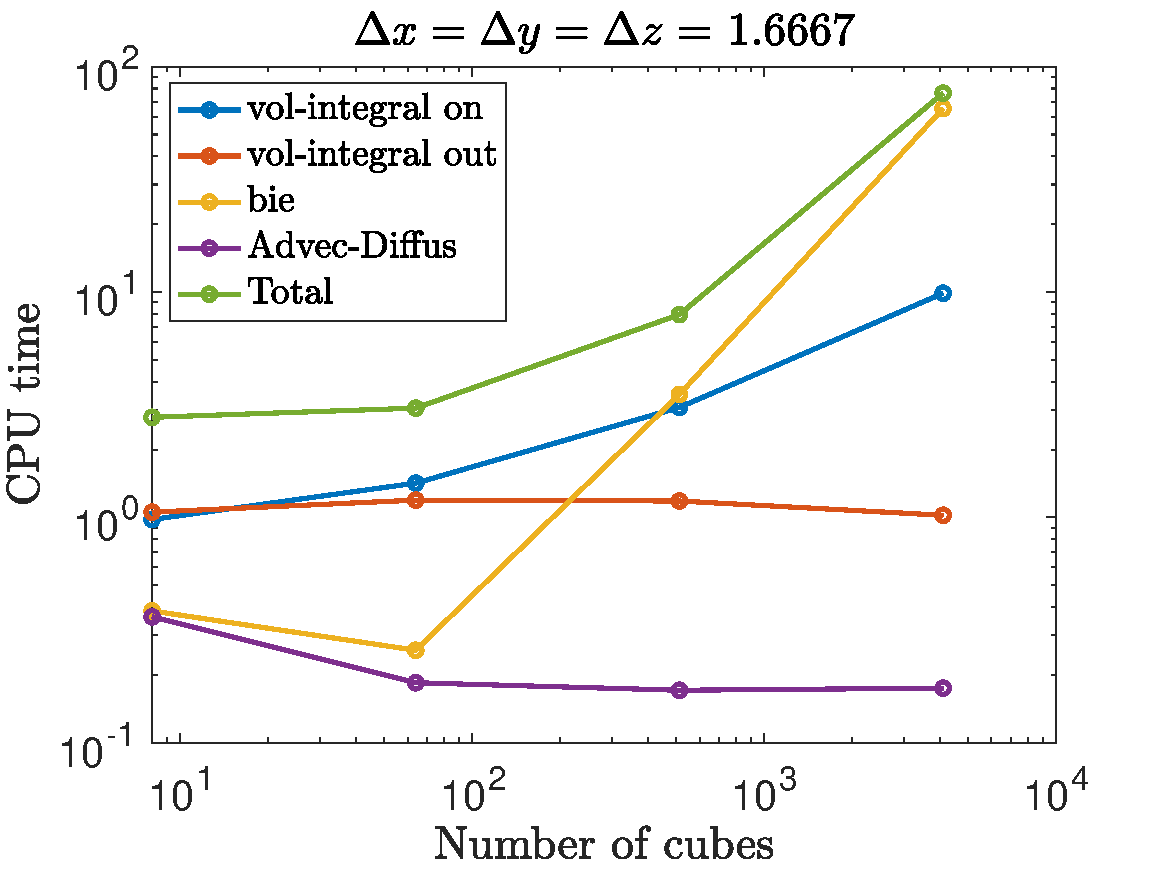
\includegraphics[scale=0.5]{./figures/fig_test_time1_fixNx}
	
	\caption{Fixed fluid domain size.}
	\label{fig_test_time1_fixNx}
\end{center}
\end{figure}

\begin{figure}[h]
	\begin{center}
		\vspace{0.5cm}
		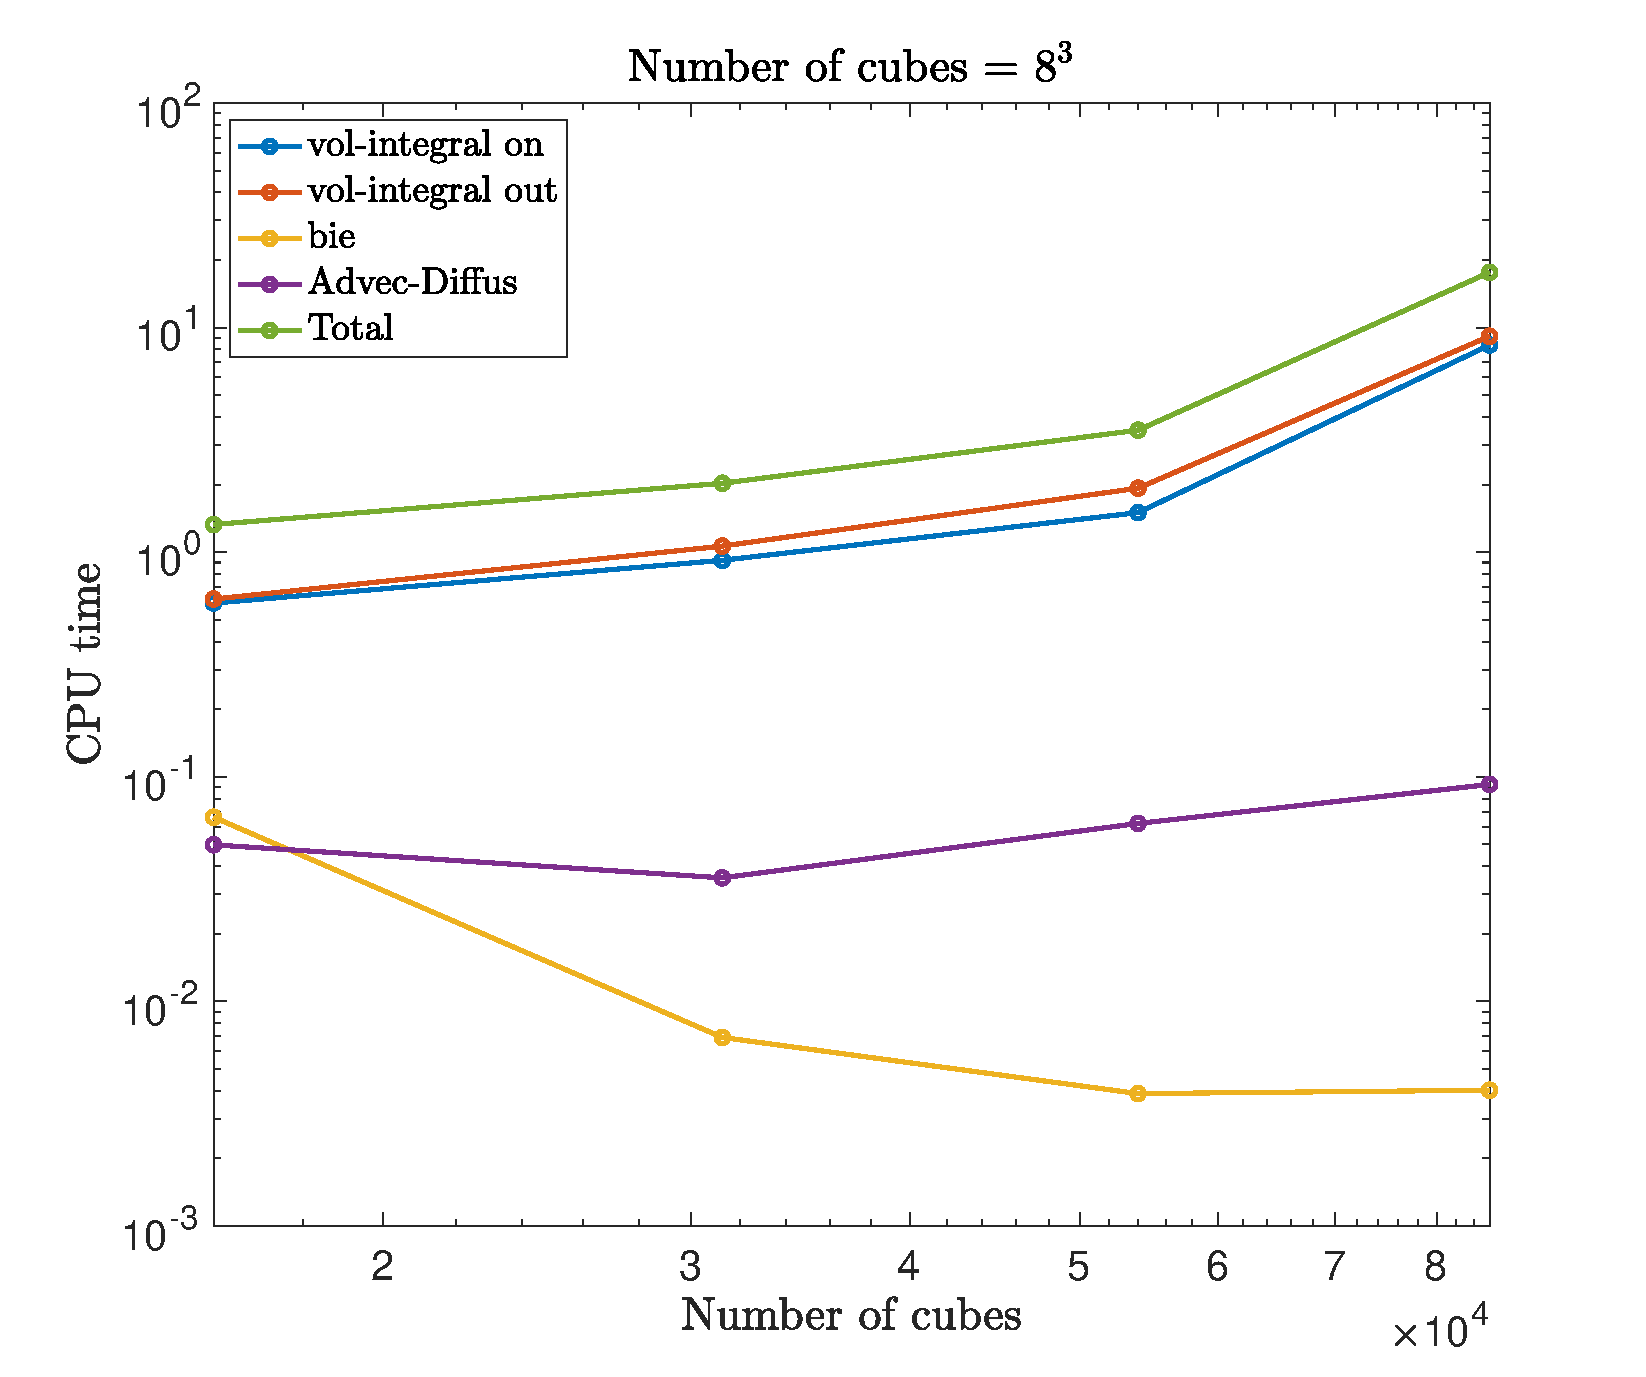
\includegraphics[scale=0.35]{./figures/fig_test_time1_varNx}
	
	\caption{Fixed aggregate size; Wrong labels. Number of cubes is $8$ and $x$-axis represents the number of total grid points. }
	\label{fig_test_time1_varNx}
\end{center}
\end{figure}

\clearpage
Today is 09/06/2022. We ran 10 time-steps for each case. The following is the setting I used to check the runtime. 
\begin{framed}
	\begin{itemize}
		\item Reference length scale: $L = 5 \times 10^{-4}$(m).
		\item Gravitational acceleration $g = 9.8$ (m$/$s$^2$).
		\item $\tilde{\mu} = 1.2 \times 10^{-3}$ (kg$/$ ms) .
		\item $\rho_s = 1.4 \times 10^{3}$ (kg$/$ m$^3$) .
		\item $\rho_0 = 1.025 \times 10^{3}$ (kg$/$ m$^3$) .
		\item $\phi = 0.9999$
		\item $\gamma = -10^{-5}$.
		\item $\alpha = 1$.
		\item $C(\vec{x}, 0) = 0$ (everywhere).
		\item Peclet number = 50.
		\\
		\item \verb+Nx = [2^3, 2^4, 2^5, 2^6]+
		\item \verb+Ny = Nx, Nz = 2Nx+
		\item Fluid domain size: $[-20, 20] \times [-20, 20] \times [-40, 40]$
		\item \verb+dt = 0.1+
		\item \verb+Nt = 10+
		\item Rotation off 
		\item \verb+NC = 8+ (Cube shape)
	\end{itemize}
\end{framed}
\begin{figure}[h]
	\begin{center}
		\vspace{0.5cm}
		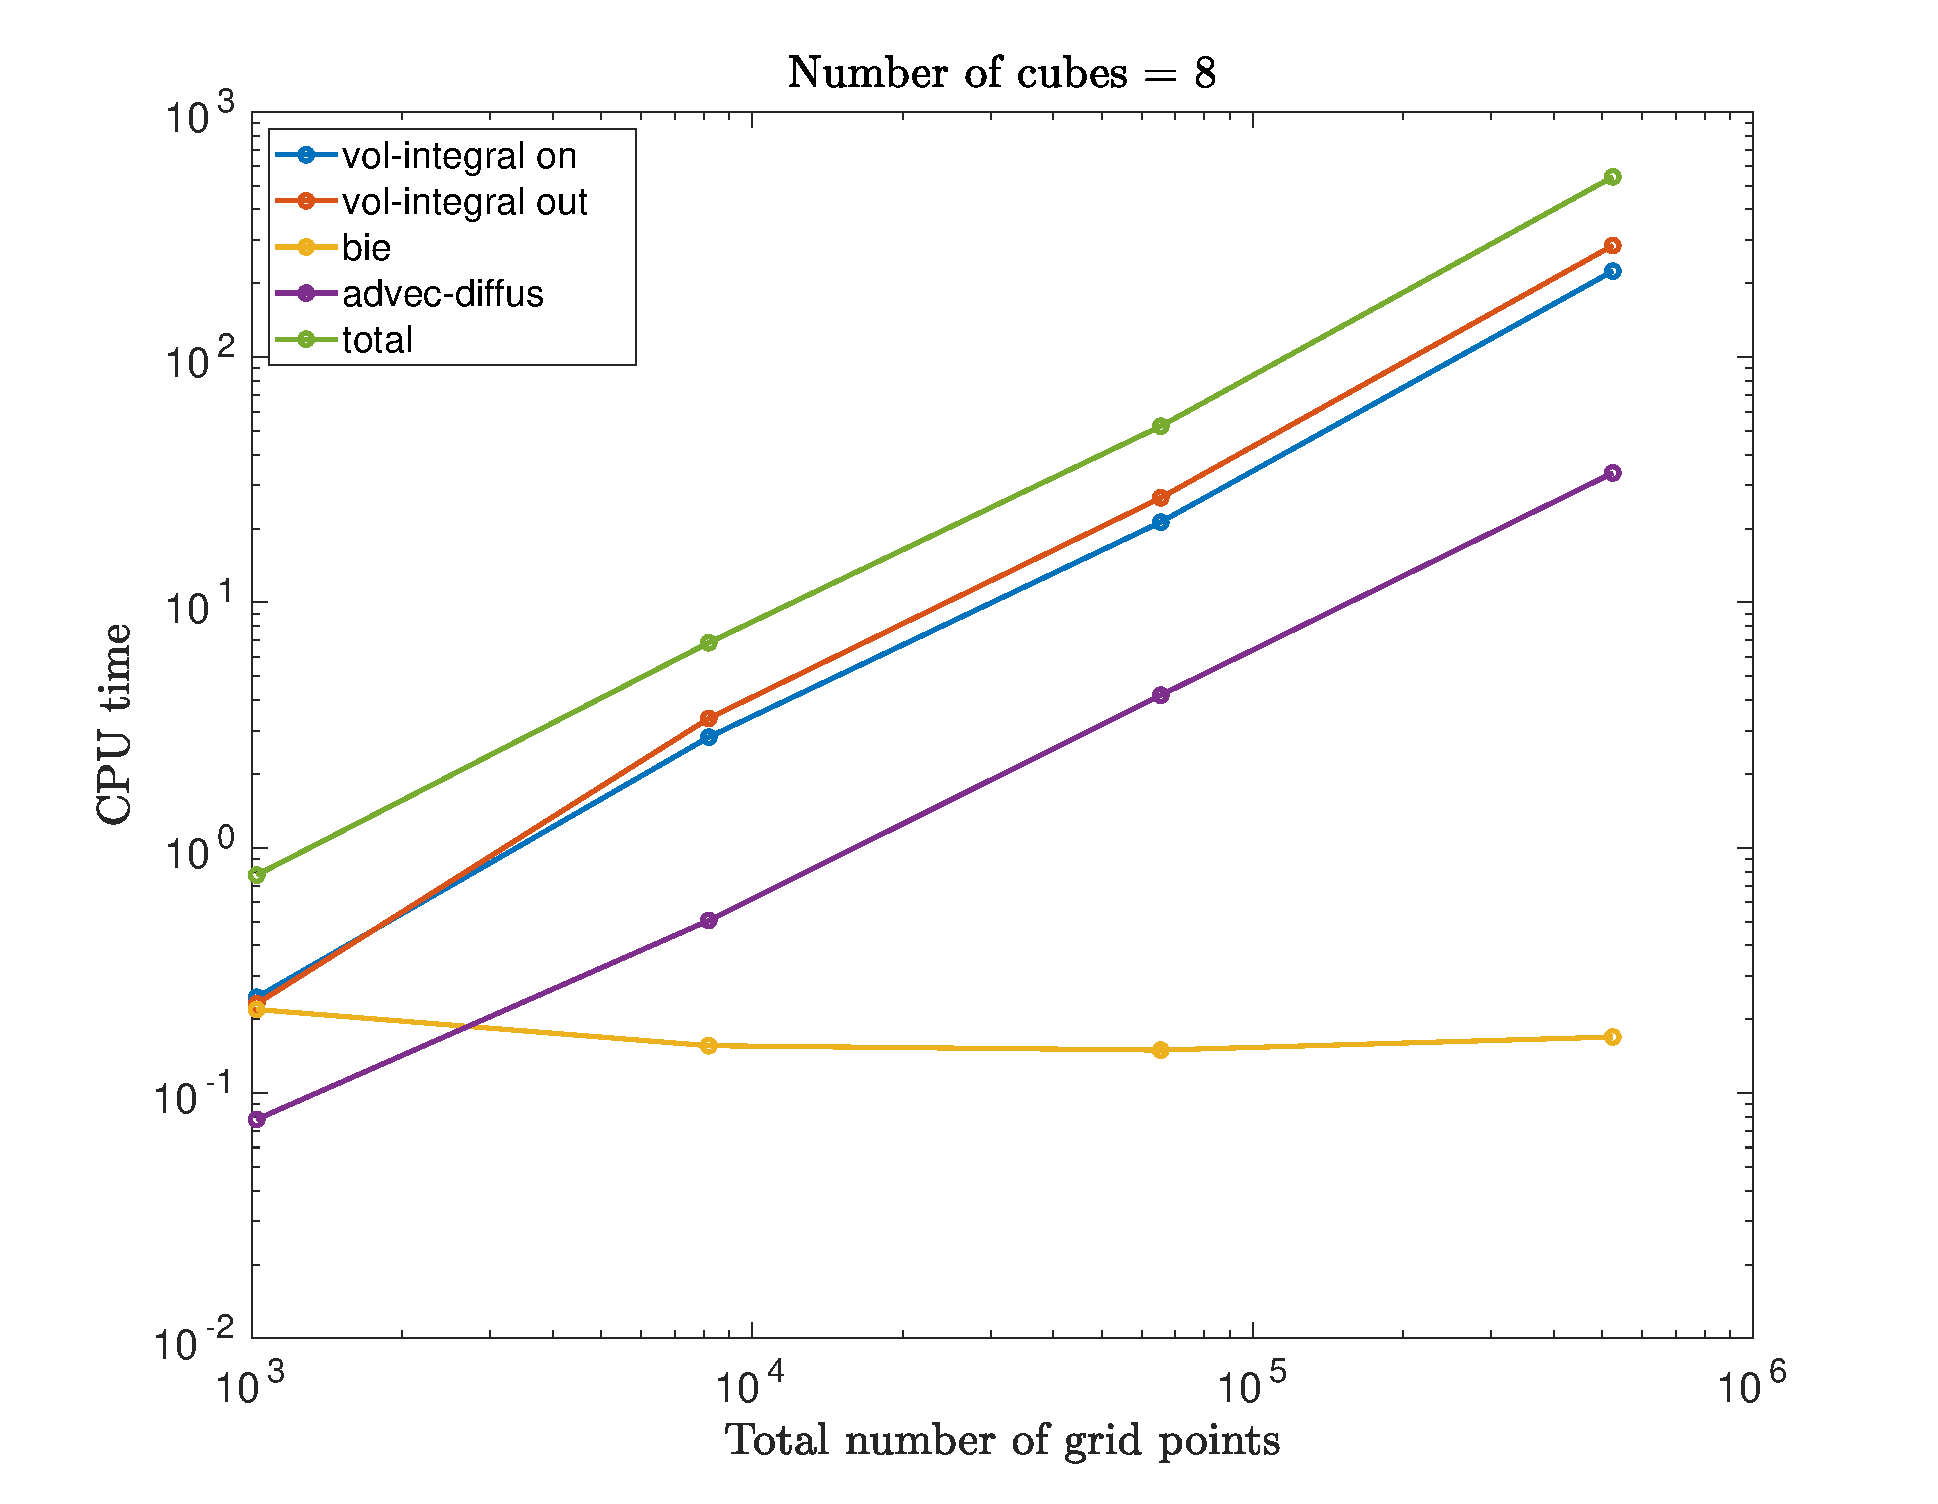
\includegraphics[scale=0.3]{./figures/fig_10time_NC8_varNx}
	
	\caption{Number of cubes is 8. }
	\label{fig_10time_NC8_varNx}
\end{center}
\end{figure}
%
% \begin{figure}[h]
% 	\begin{center}
% 		\vspace{0.5cm}
% 		\includegraphics[scale=0.33]{./figures/fig_10time_NC125_varNx}
% 		\includegraphics[scale=0.33]{./figures/fig_vel_test2-2}
	
% 	\caption{Number of cubes is 125. }
% 	\label{fig_10time_NC125_varNx}
% \end{center}
% \end{figure}
\clearpage
[Updated on 01/26/2023]
%
% \begin{figure}[h]
% 	\begin{center}
% 		\vspace{0.5cm}
% 		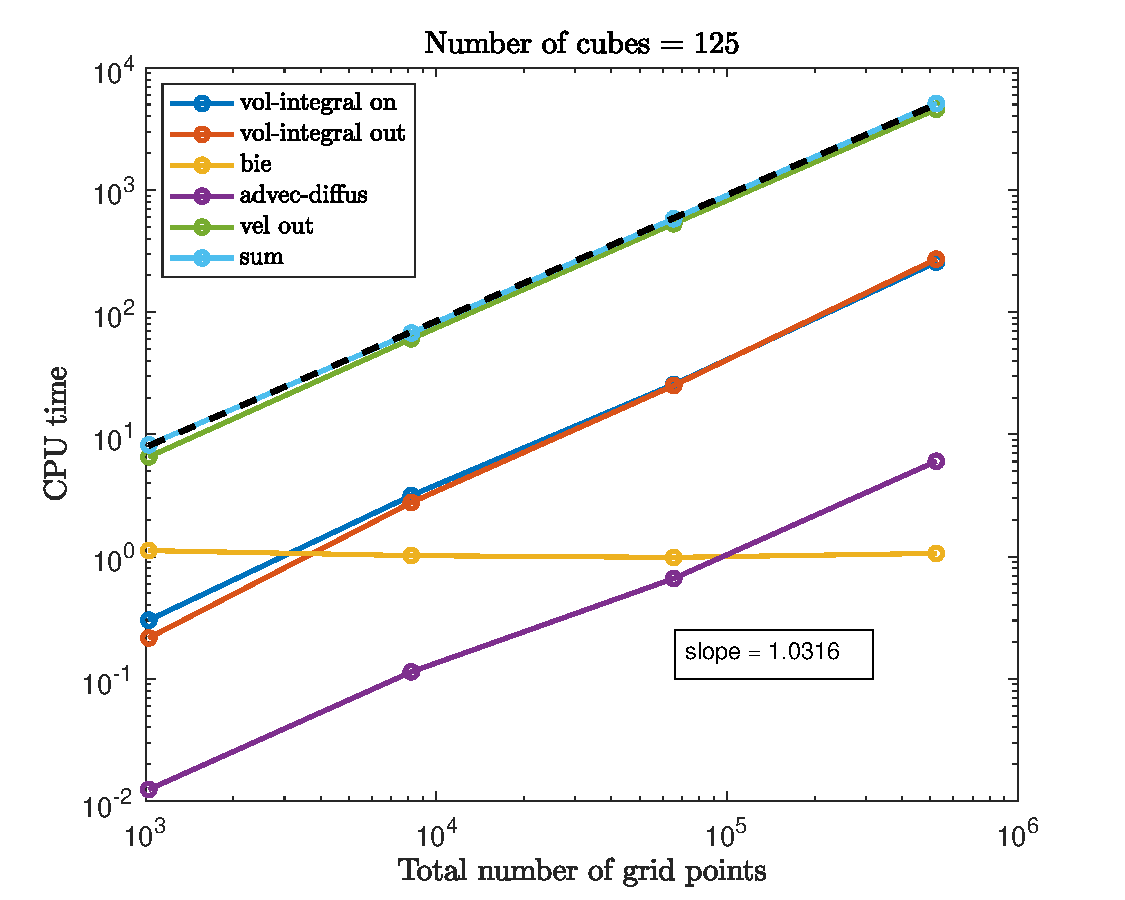
\includegraphics[scale=0.5]{./figures/fig_time_varNx5}	
% 	\caption{Number of cubes is 125.}
% 	\label{fig_time_varNx5}
% \end{center}
% \end{figure}
\begin{figure}[h]
	\begin{center}
		\vspace{0.5cm}
		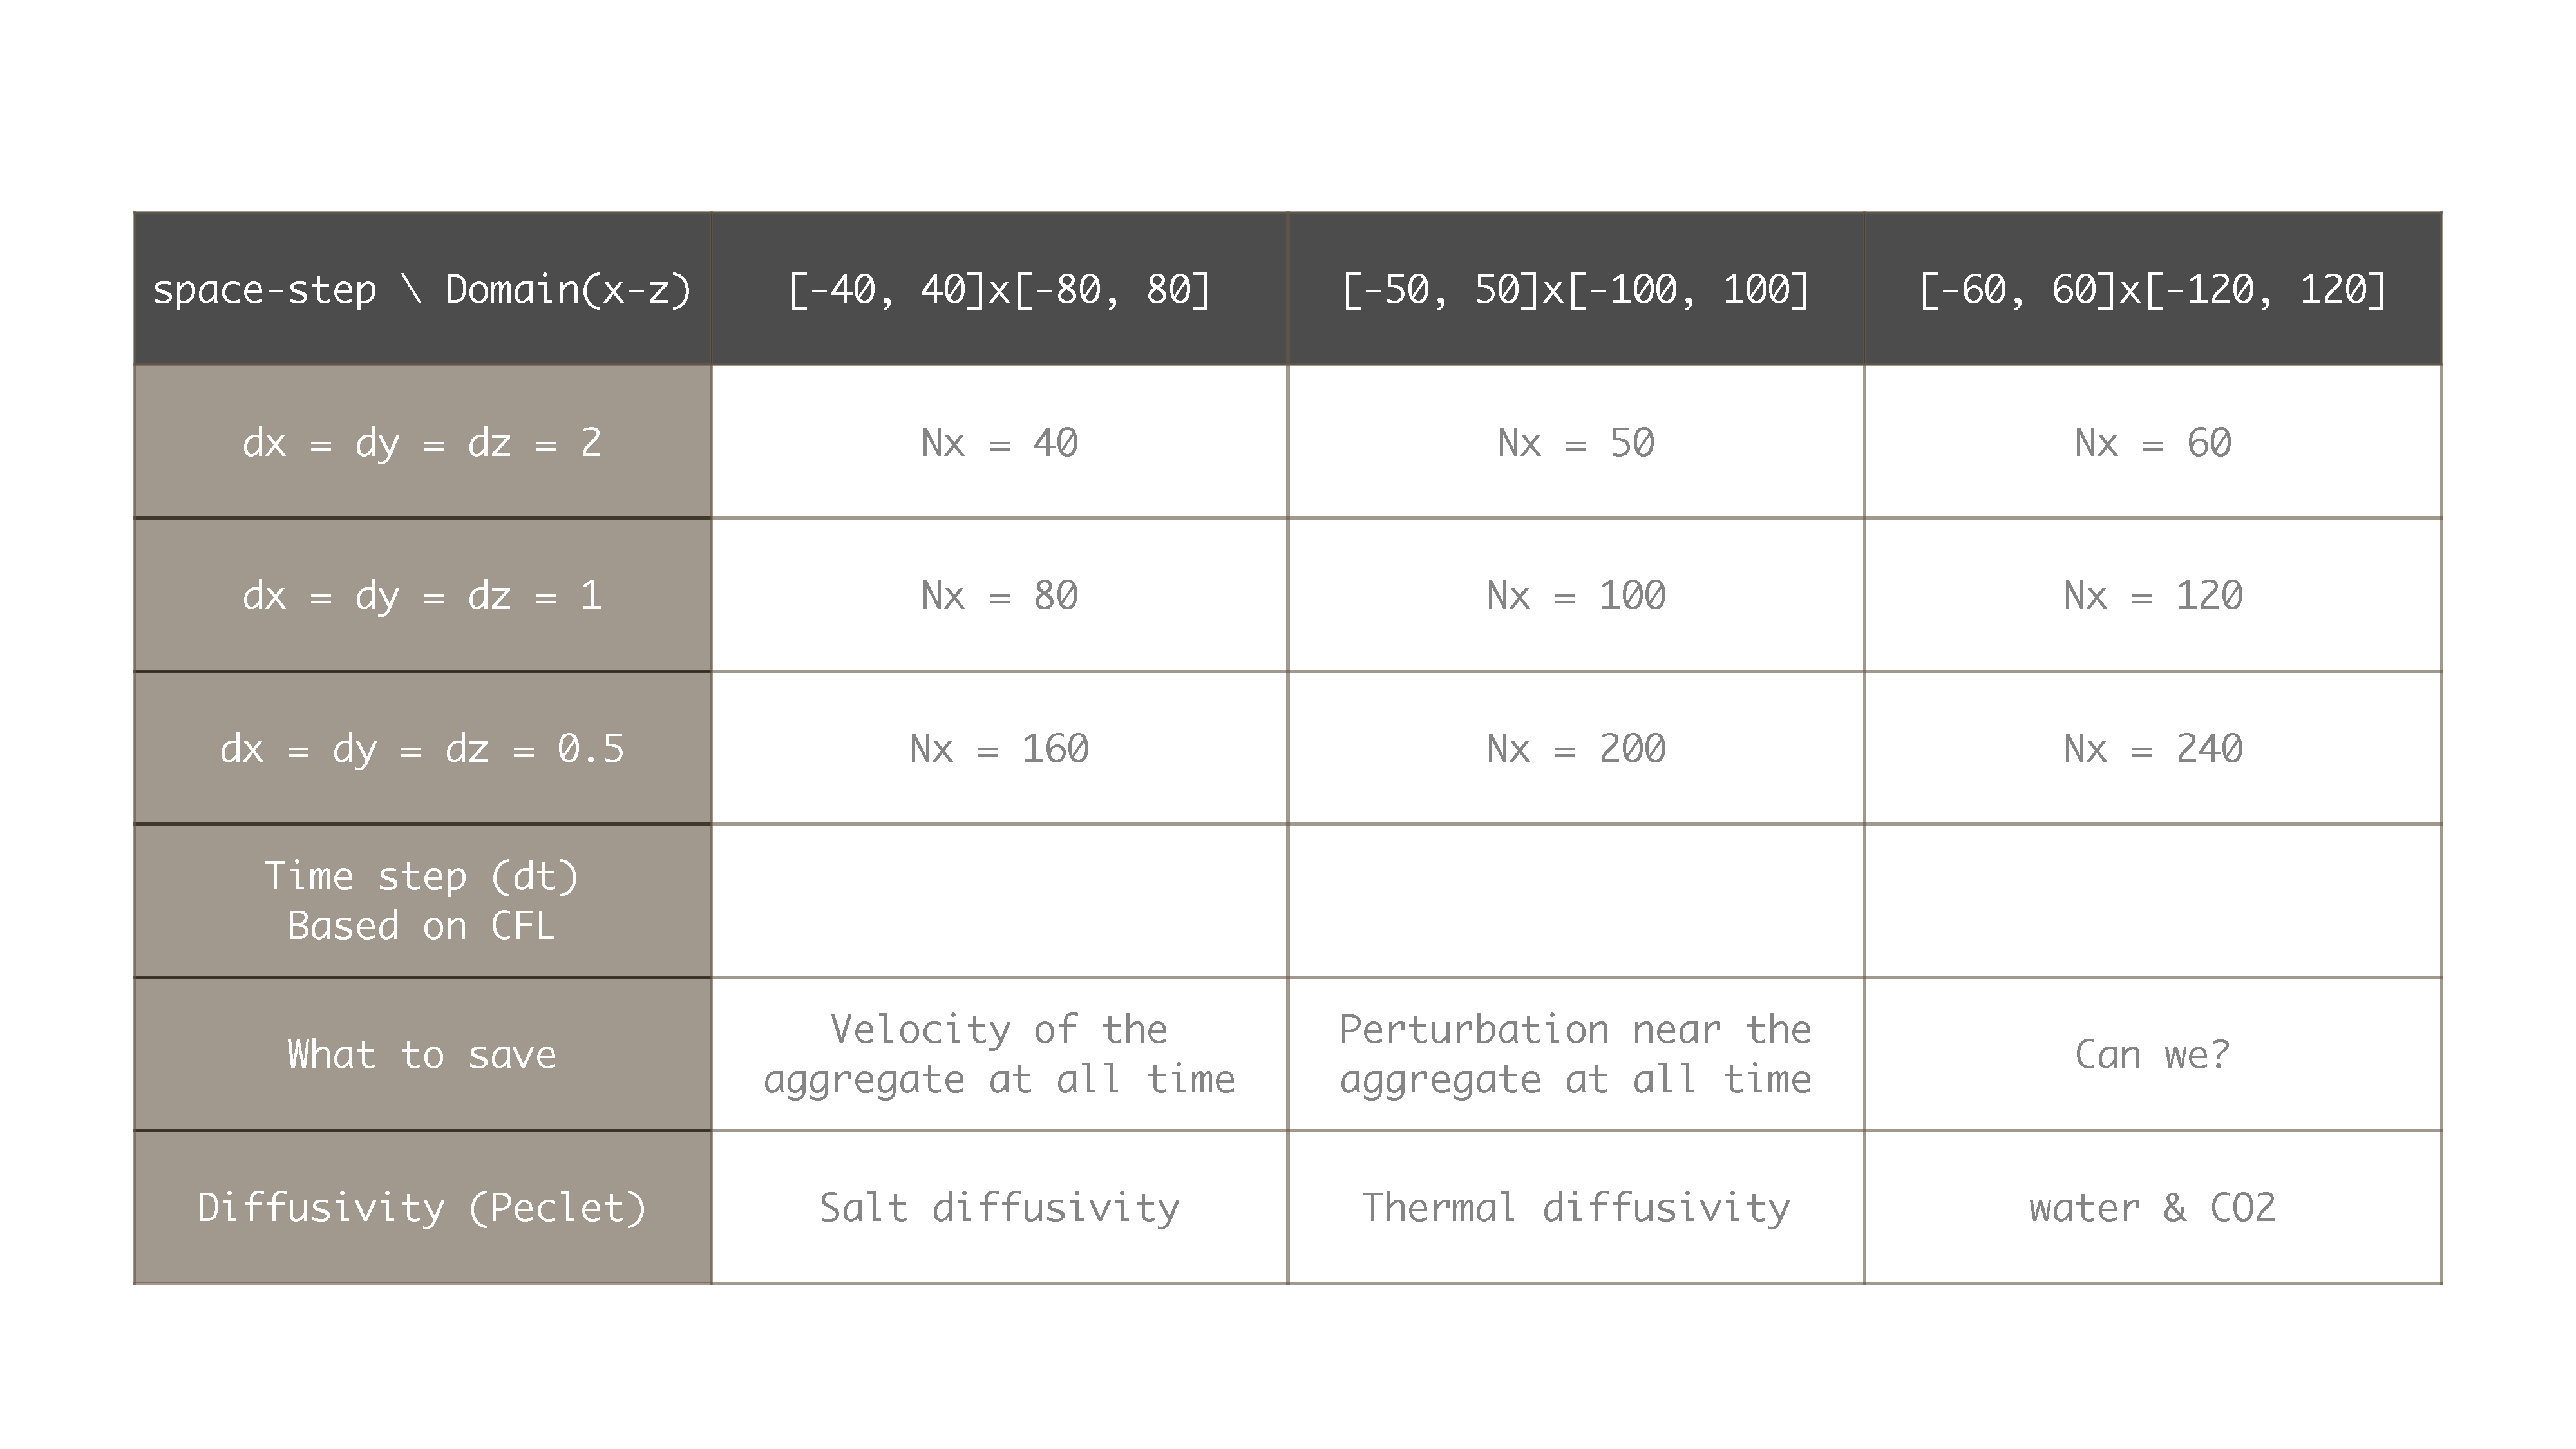
\includegraphics[scale=0.25]{./figures/table_agg_MERCED}	
	\caption{What we should run.}
	\label{fig_map_MERCED}
\end{center}
\end{figure}
\\
How can we determine the time-step size, $\Delta t$? We need to consider CFL here, for both advection and diffusion. 
\\
Knowing that the unit of diffusivity is [D] = $L^2/T$, we consider 
\[
R_{max}^2 \sim \text{Pe} \Delta t,
\]
wherer $R_{max}$ is a maximum radius of the aggregate. 
\end{comment}
\subsection{Homogeneous velocity computation with FMM}
We noticed that the homogeneous velocity computation using the boundary integral equation is quite slow, due to the large number of fluid domain grid points. We thus attempt to use the fast multipole method (FMM) for this surface integral, by approximating as following:
\begin{equation}
	u_H(\vec{y})  
	= \int_S \vec{f}(\vec{x}) \cdot \bar{\bar{G \ }}( \vec{x}, \vec{y}) \ \text{d} S(\vec{x}),
	\label{eq_uH}
\end{equation}
where $\vec{y}$ is points in the fluids, outside of the aggregate boudnary. Note that we call $\vec{x}$ as source, since they are on the integral domain, and $\vec{y}$ as target point. 
For the velocity inside and on the aggregate boundary, we use the rigid boundary velocity $u(\vec{x}) = \vec{U}_a + \vec{\Omega} \times \left(\vec{x} - \vec{x}_{cm} \right)$. This implies that we do not expect any singularity in this computation ($\vec{x} \neq \vec{y}$), however, we may have close evaluation problem. We will discuss the size of error in the next section. 
% Let $r_{nm} = \|\vec{x}^n - \vec{y}^m \|$. 
\par
Using the Laplace kernel, we can re-write the surface integral (\ref{eq_uH}) as
\begin{equation}
	u_H(\vec{y}) =
	\int_S 
	\vec{f}(\vec{x}) \cdot
  	\left(
  	\frac{\bar{\bar{I \ }}}{\|\vec{x} - \vec{y}\|}
  	- \left( \vec{x} - \vec{y} \right)
  	 \nabla_{\vec{x}}
  	\frac{1}{\|\vec{x} - \vec{y}\|}
  	\right)
	  \ \text{d} S(\vec{x}).
 \label{eq_surf_laplace}
\end{equation}
We first discretize the entire aggregate surface into $Nf$ number of square faces that are located at $[cx_1^n-1, cx^n_1+1] \times [cx^n_2-1, cx^n_2+1]$. This refers that $(cx^n_1, cx^n_2)$ is the center of $n-$th square face. The discretized version of the velocity equation (\ref{eq_surf_laplace}) is denoted by $H(\vec{y})$,
\begin{align}
	H(\vec{y}^m) & = u_H(\vec{y}) - E_f
	 = \sum_{n = 1}^{Nf} H^n(\vec{y}^m) 
	\nonumber \\
	& = \sum_{n = 1}^{Nf} 
	\vec{f}(\vec{x}^n) \cdot
	\int_{cx^n_2-1}^{cx^n_2+1} \int_{cx_1^n-1}^{cx_1^n+1}
  	\left(
  	\frac{\bar{\bar{I \ }}}{\|\vec{x}^n - \vec{y}^m\|}
  	- \left( \vec{x}^n - \vec{y}^m \right)
  	 \nabla_{\vec{x}^n}
  	\frac{1}{\|\vec{x}^n - \vec{y}^m\|}
  	\right)
	  \text{d} x_1  \text{d} x_2
	  ,
 \label{eq_surf_fmm_Nf}
\end{align}
where $m = 1, \  2, \cdots, \ M$, and $M$ is the total number of targets (where we want to obtain the velocity).  Note that the stress $\vec{f}(\vec{x}^n)$ is assumed to be constant over each square face. The error coming from this approximation is denoted as $E_f$; its error analysis is discussed in our previous paper \cite{yoo_hydrodynamic_2020}. One can find that we have the largest error at the corner of the cube. We would like to keep this true as we make further approximation. 
%We may begin using the FMM3D code for each $\vec{x}^n$ for now (using the FMM3D $Nf$ times {\color{red} $\rightarrow$ This is fixed now. Total 18 times we use. how did you do it?}). We should be able to edit the code for efficiency. 
% Since we need to compute two terms inside of the itnegral separately,
\par
Next, we need to approximate the surface integral in equation (\ref{eq_surf_fmm_Nf}) using a Riemann sum,
% {\color{blue} We should perform an error analysis for this entire computation.}
% For the simplicity, we first consider the integral over one square face. 
% For each $n$, we have
\begin{align}
	\tilde{H}^n(\vec{y}^m) 
	& = H^n(\vec{y}^m) - E_{G} 
	\nonumber \\ 
	& =
	\sum_{n = 1}^{Nf} 
	\vec{f}(\vec{x}^n) \cdot
	\sum_{s=1}^{Ns^2} d^2 
  	\left(
  	\frac{\bar{\bar{I \ }}}{\|\vec{x}_s^n - \vec{y}_s^m\|}
  	- \left( \vec{x}_s^n - \vec{y}^m \right)
  	 \nabla_{\vec{x}_s^n}
  	\frac{1}{\|\vec{x}_s^n - \vec{y}^m\|}
  	\right)
	  + E_{G},
 \label{eq_surf_fmm_Nf_n}
\end{align}
where $E_G$ is the error coming from the quadrature method. 
We make $Ns$ number of sub-squares, that have sizes of $d = 2/Ns$, and take the center of each sub-squares as the integration points. 
We take the same number of points, $Ns$, evenly distributed, in one direction. We can also consider the number points as the number of sub-squares in one face. 
In the following schematics, Figurue \ref{fig_face_grid}, the red cross represents the center of the $n-$th square face, $(cx^n_1, cx^n_2)$.
\begin{figure}[h]
	\begin{center}
		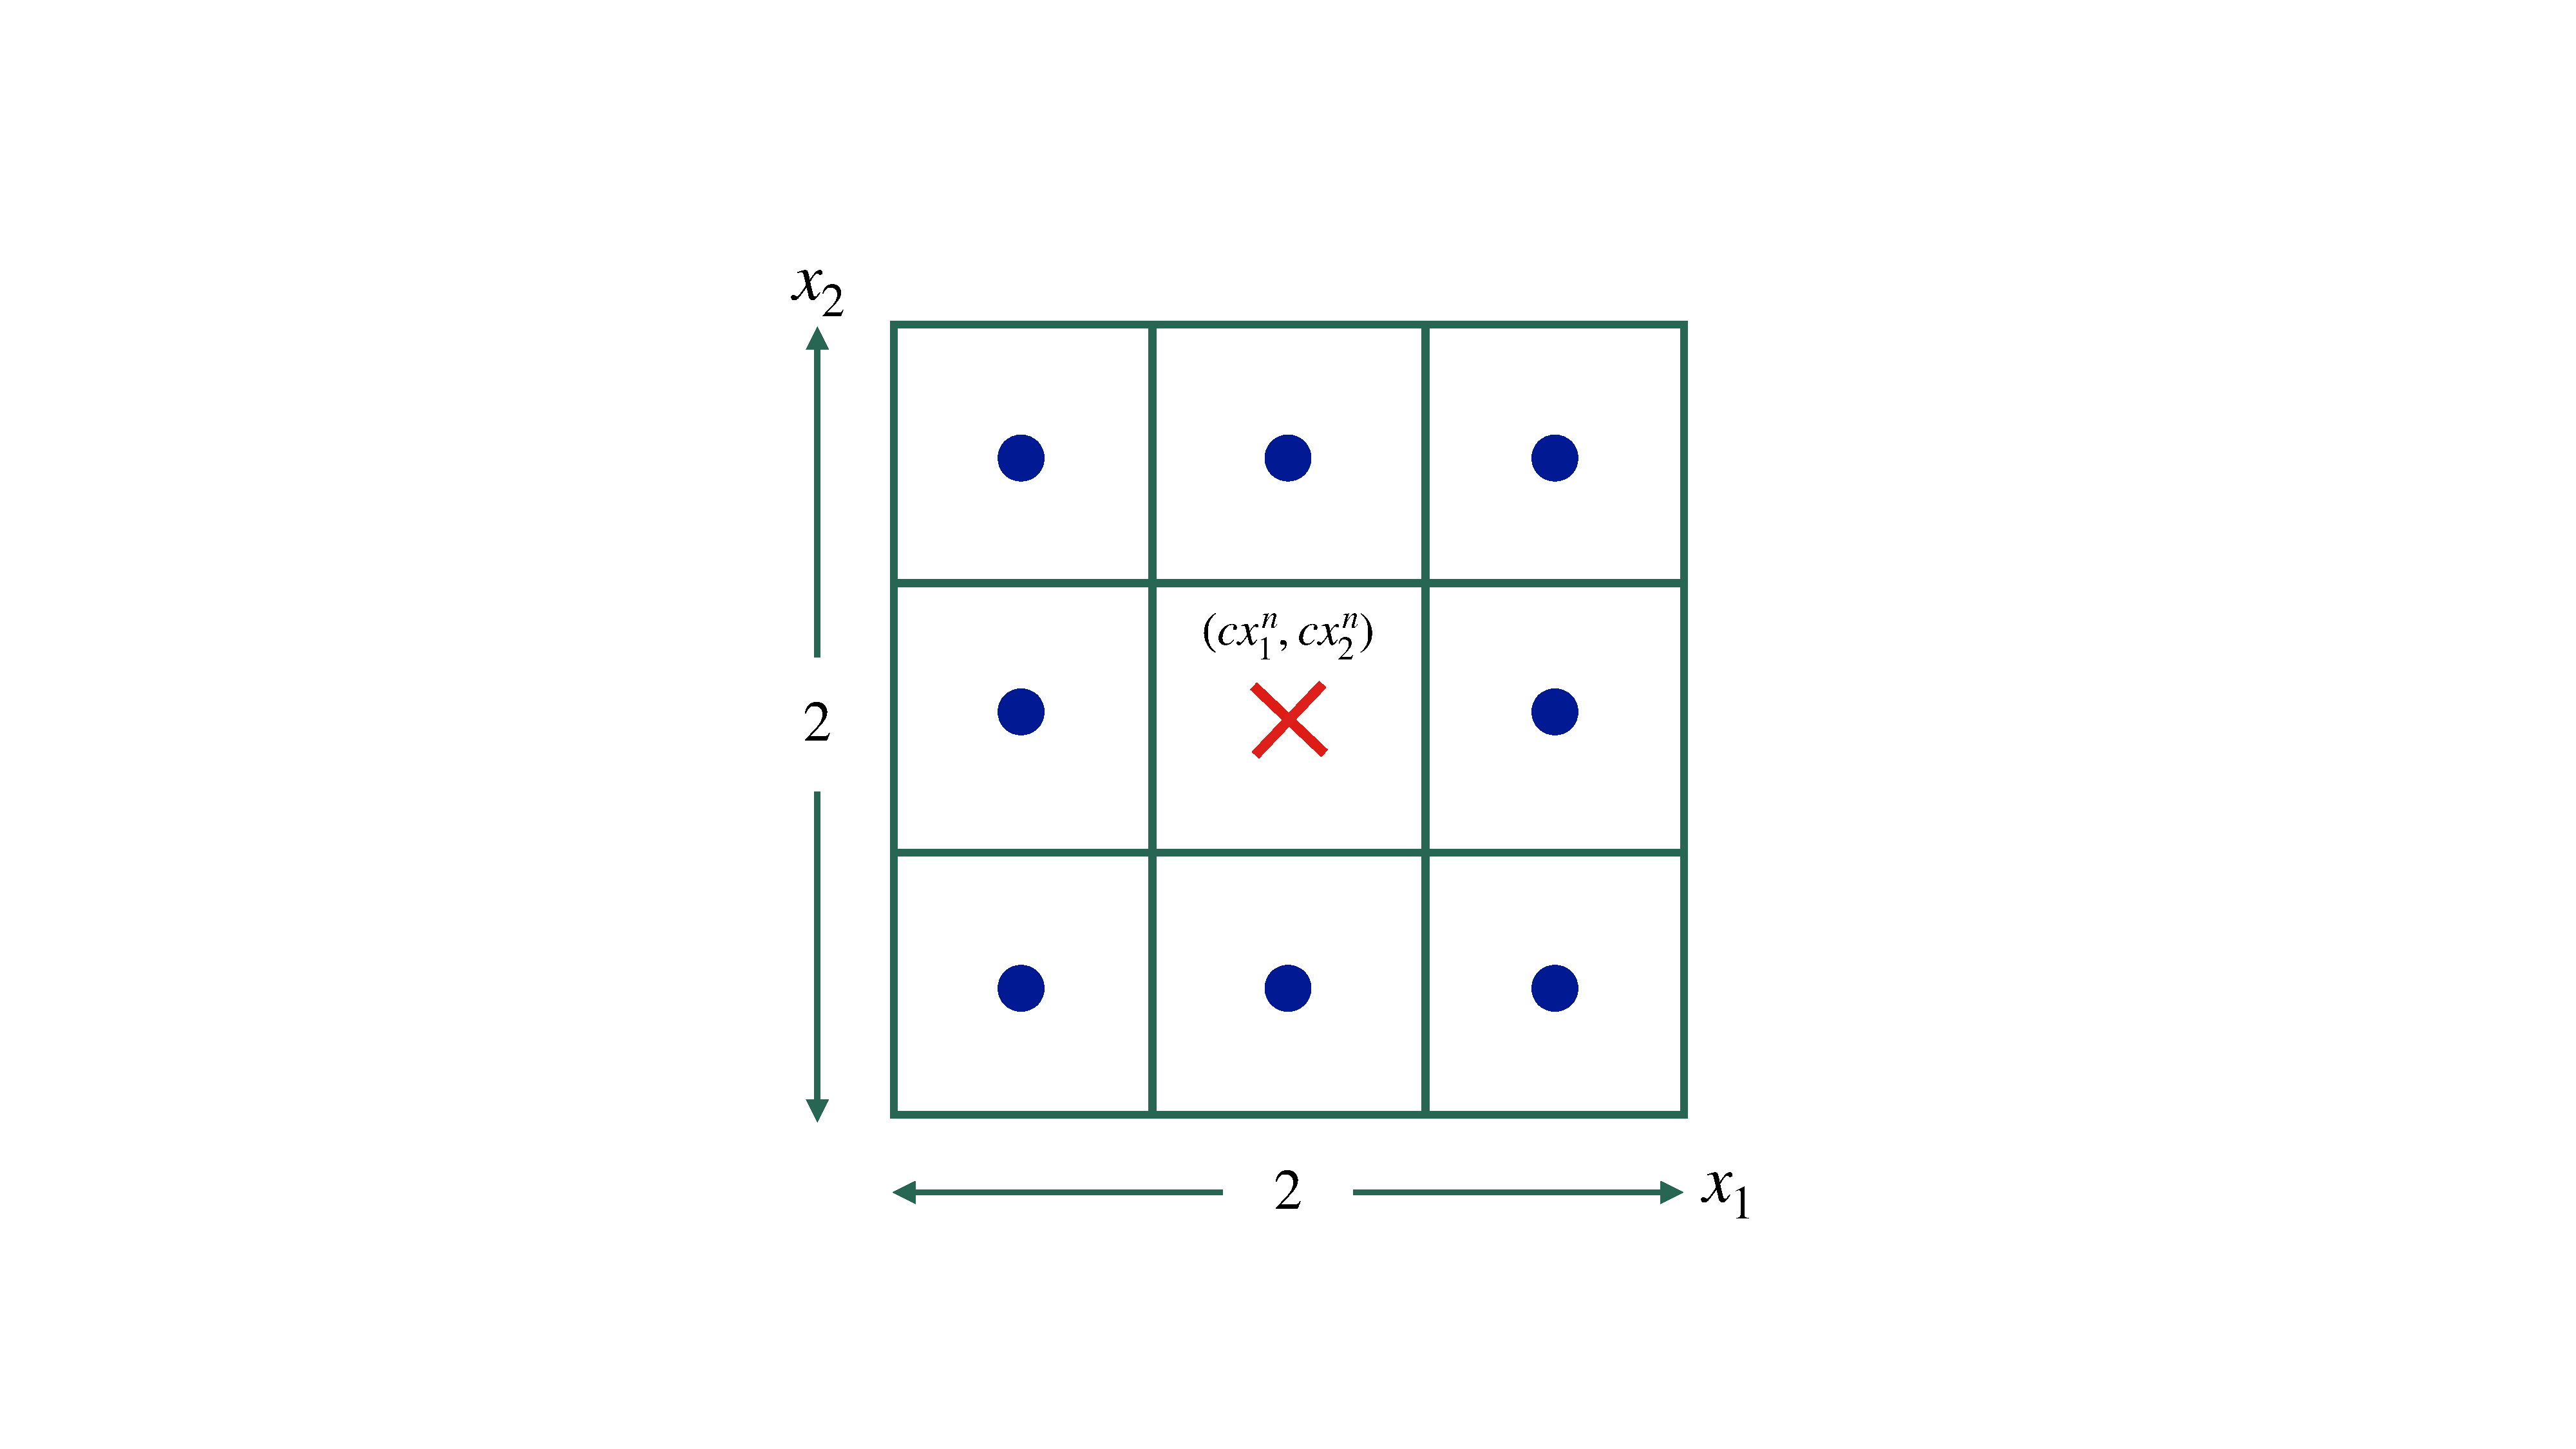
\includegraphics[scale=0.17]{./figures/fig_face_grid}
	\caption{Schematic of points we use to approximate the integral of the single-layer potential kernel over one square face.}
	\label{fig_face_grid}
\end{center}
\end{figure}
Including the center, that is the red cross, the blue dots are the integration points.
% For the horizontal, $x_1$-direction, we create an array as \verb+x1 = -floor(Ns/2):floor(Ns/2)+, and the  coordinates of those points are \verb+x1Span = cx1 + d.* x1+
For simplicity, we may not include any boundary values on one square face.
\par
% \subsection{Error analysis}
As we mentioned, we hope to have a reasonable size of the integration error, $E_G \ll E_f$.
In order to measure $E_f$, we consider the settling of one cube shape aggregate.
We then observe the relative error of the vertical velocity on one square face, considering the translational velocity, $\vec{U}_a$, as the exact solution. Note that we do not have rotation, i.e., $\vec{\Omega} = \vec{0}$. 
\begin{figure}[h]
	\begin{center}
		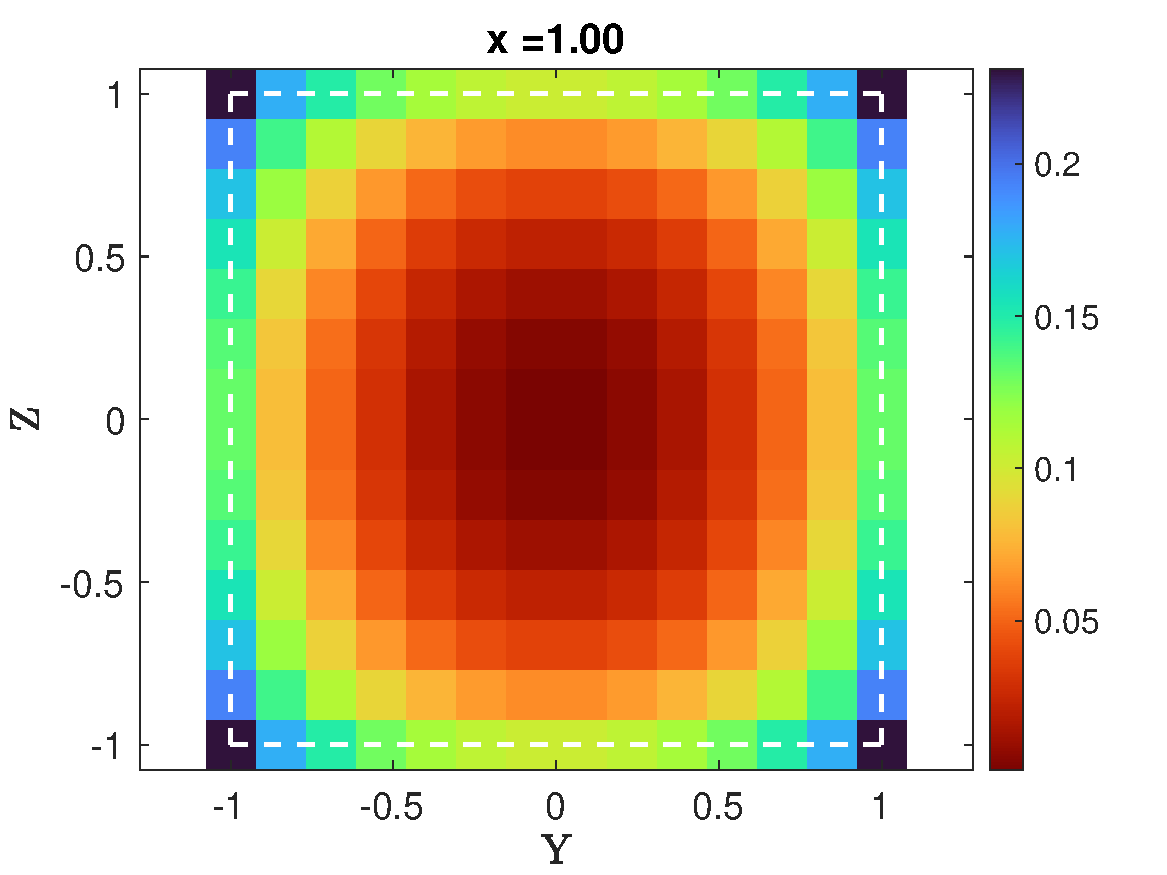
\includegraphics[scale=0.3]{./figures/fig_corner_err}
	\caption{Relative error of }
	\label{fig_corner_err}
\end{center}
\end{figure}
In figure \ref{fig_corner_err}, we see the square face at $x = 1.00$, where the white dashed line shows the location of the square face, and the color shows the relative error. It implies that the maximum of 23.12$\%$ error occurs at the corner of the cube, as we expected. We thus would like to regulate the quadrature error, $E_G$, accordingly by adjusting the total number of integration points, $Ns^2$.
\par
{\bf To clarify what we want to do:}
Let $u_H(\vec{y})  = U = F \cdot  G$ be the exact or true velocity computation. Then 
\begin{align}
	U^* = F^* \cdot  G
	\\
	U^{*+} = F^* \cdot  G^+
\end{align}
where $F = F^* + E_f$ and $G =  G^+ + E_G$.
By approximating the integral of the kernal, using FMM3D, we compute $U^{*+}$, that is,
\begin{align}
	U^{*+} = (F-E_f) \cdot (G - E_G) 
	% \nonumber \\
	% = F \cdot G - F \cdot E_G - G \cdot E_f 
	% + E_f \cdot E_G
	% \\
	= U +  \left| E_f \cdot G + F  \cdot E_G \right|  + \mathcal{O}(E_f E_G).
\end{align}
We know that 
\[
	|U-U^*| = |E_f \cdot G| \approx 23 \%,
	\]
and we would like to have
\[
	|F  \cdot E_G| \ll	|E_f \cdot G |
\]
Note that 
\[
	  |F \cdot E_G| = |F^* \cdot E_G + E_f \cdot E_G|
	  \approx |F^* \cdot E_G |
\]
Thus, what we need to compare is two velocity approximations,
\begin{align}
	|U^* - U^{*+}| =| F^* \cdot E_G| \ll 23 \%
	\label{eq_condition_EG}
\end{align}
We vary the number of integration points to choose an optimal value. For this experiment, we set $\varepsilon = 10^{-6}$.
\begin{figure}[ht]
	\begin{center}
		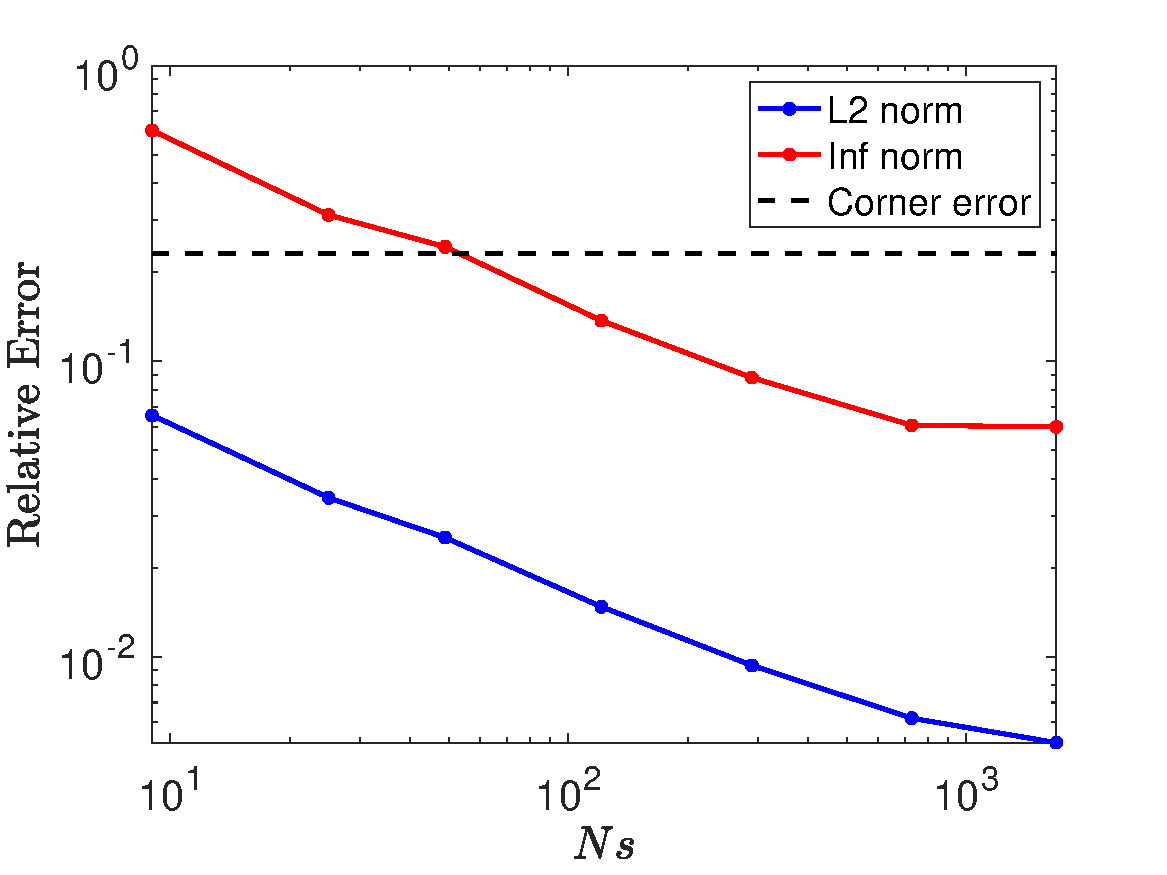
\includegraphics[scale=0.33]{./figures/fig_Ef_EG_compare}
	\caption{Relative error between $U^*$ and $U^{*+}$, varying the number of integration points: $Ns = [3, 5, 7, 11, 17, 27,41]^2$. Set $\varepsilon = 10^{-6}$.}
	\label{fig_Ef_EG_compare}
\end{center}
\end{figure}
Figure \ref{fig_Ef_EG_compare} shows that $Ns = 9^2$ points are enough to satisfy what we needed in equation (\ref{eq_condition_EG}). 
\par
When we use FMM3D library, we can choose the desired accuracy, $\varepsilon$, which determines the number of terms in the series expansion. We do not want to select too small $\varepsilon$ since it increases the computation time. Since we used $\varepsilon = 10^{-6}$ to produce figure \ref{fig_Ef_EG_compare}, we set $\varepsilon = 10^{-1}$ to see the difference. As we can see in figure \ref{fig_Ef_Eg_ep-1}, there is no difference in accuracy with higher $\varepsilon$. The reason we guess is because the corner error, $E_f$, is dominating in our approximation and it is already larger than $10 \%$. 
\begin{figure}[ht]
	\begin{center}
		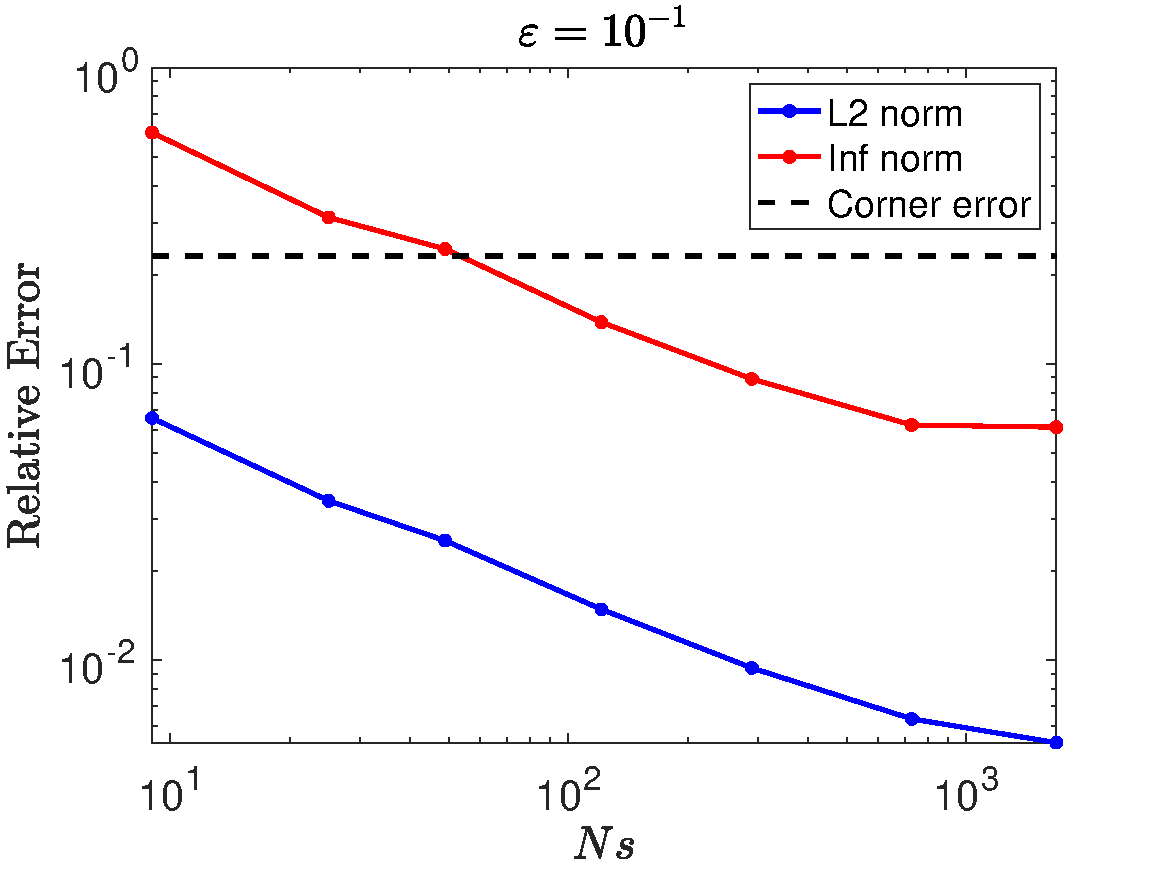
\includegraphics[scale=0.33]{./figures/fig_Ef_Eg_ep-1}
	\caption{Relative error between $U^*$ and $U^{*+}$, varying the number of integration points: $Ns = [3, 5, 7, 11, 17, 27,41]^2$. Set $\varepsilon = 10^{-1}$.}
	\label{fig_Ef_Eg_ep-1}
\end{center}
\end{figure}
In order to confirm the responses of $\varepsilon$ values, we test one-time step simulation with a smaller domain size with one cube aggregate model. Here are the exact paramesters we use:
\begin{framed}
	\begin{itemize}
		\item $\varepsilon = [10^{-1}, \ 10^{-2}, \ 10^{-3}, \ 10^{-4}, \ 10^{-5}]$
		\item \verb+Nx = 41+ ($\Delta x = 0.25$)
		\item \verb+Ny = Nx, Nz = 2Nx+ 
		\item Fluid domain size: $[-5, 5] \times [-5, 5] \times [-10, 10]$
		\item \verb+Nt = 1+
		\item \verb+NC = 1+ (Cube shape)
		\item No perturbation
	\end{itemize}
\end{framed}
Here are some results. We look at the velocity field at $x = 1.125$, that is slightly outside of the aggregate. On the right, we make a slice at $z = 0$ and see the relative error considering that velocity obtained with SLP as a reference. 
\begin{figure}[ht]
	\begin{center}
		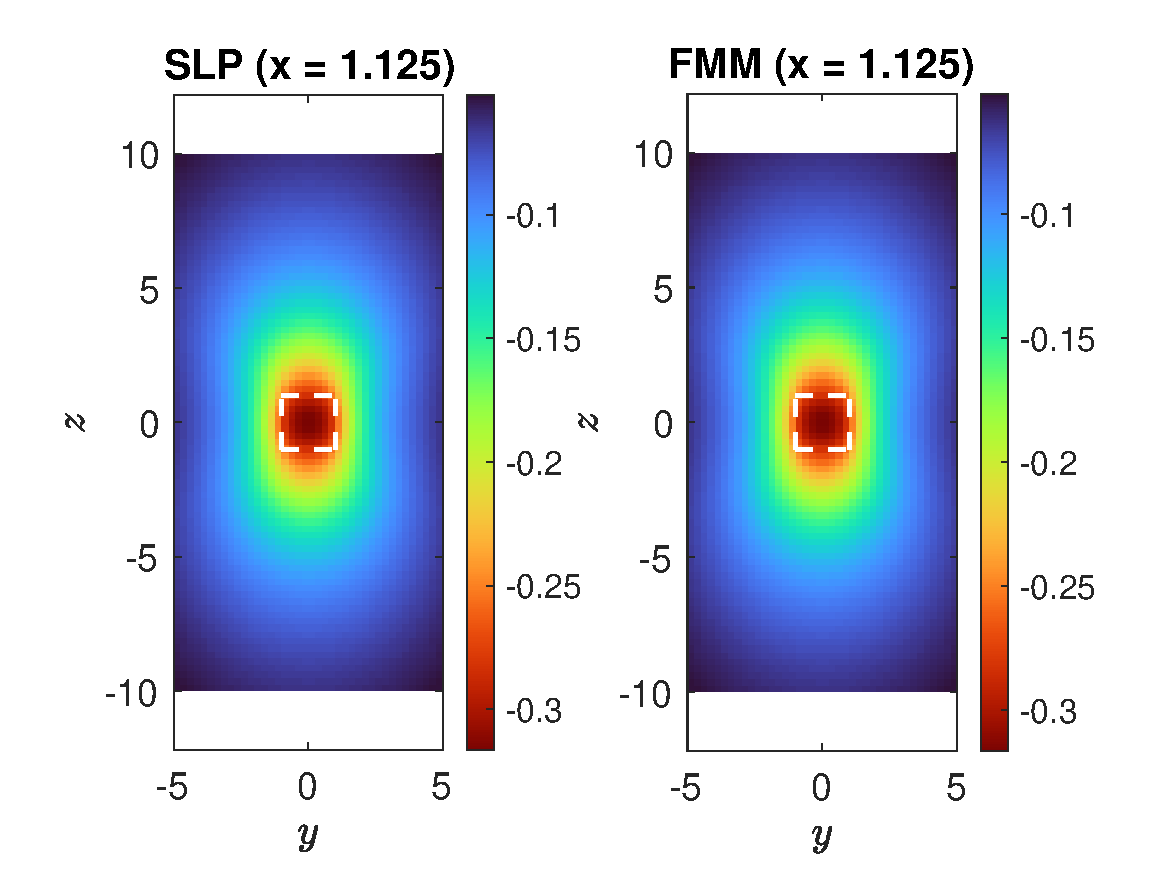
\includegraphics[scale=0.44]{./figures/fig_vel_NC1_eps1e-4}
		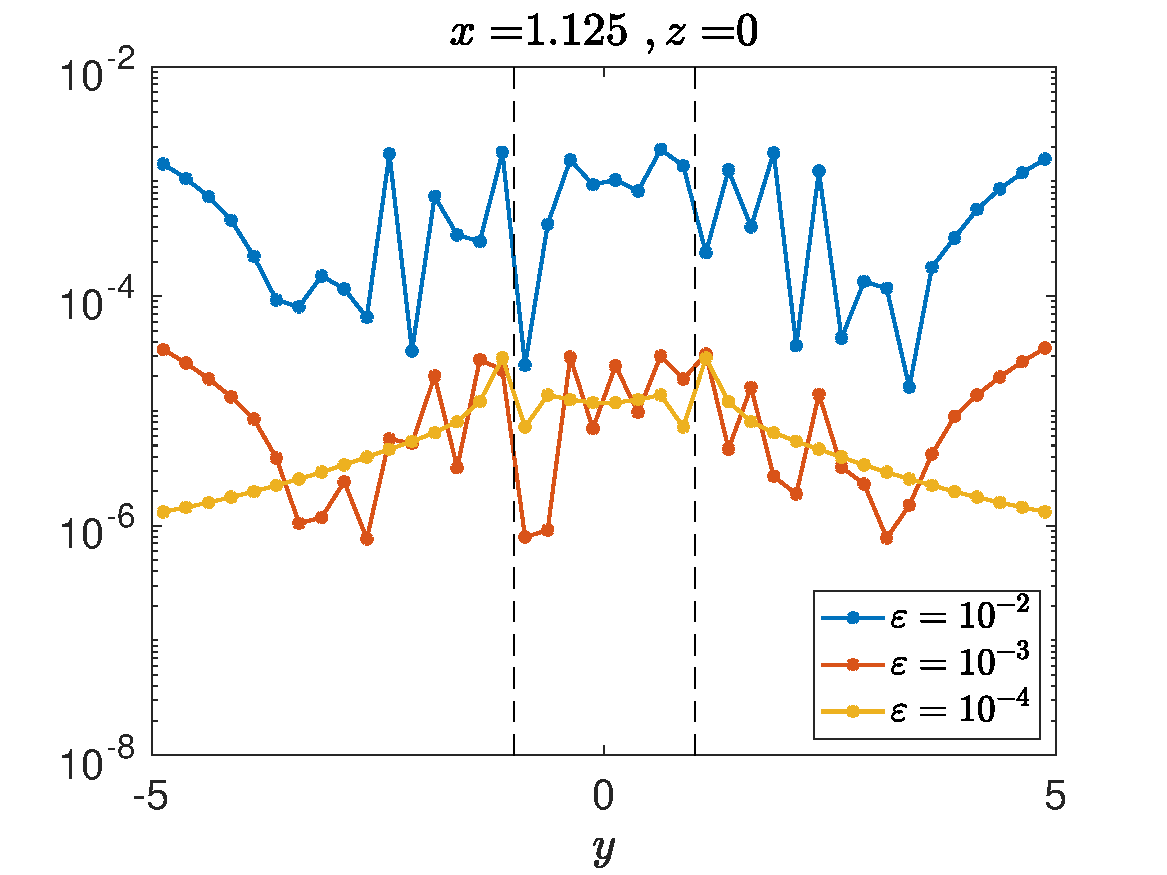
\includegraphics[scale=0.42]{./figures/fig_1Derr_NC1_eps1e-4}
	\caption{(Left) Verticle velocity field at $x = 1.125$. (Right) 1D relative error at $x = 1.125$ and $z = 0.0$ with varying $\varepsilon$.}
	\label{fig_vel_NC1_eps1e-4}
\end{center}
\end{figure}
\\
Figure \ref{fig_errNorms_varEps_NC1} shows that we may be able to obtain a good amount of error when we use $\varepsilon = 10^{-4}$. We may examine how much this choice slows the actual computation time down. 
\begin{figure}[h]
	\begin{center}
		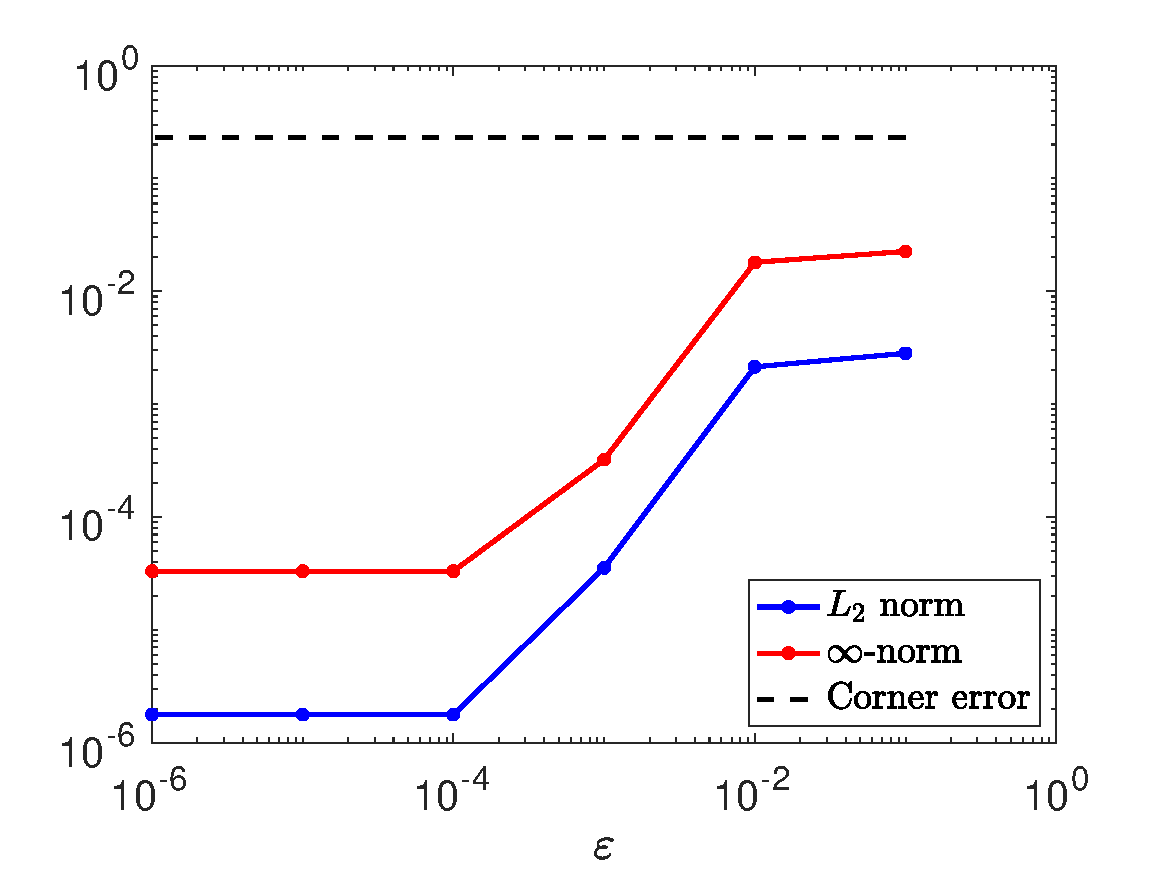
\includegraphics[scale=0.42]{./figures/fig_errNorms_varEps_NC1}
		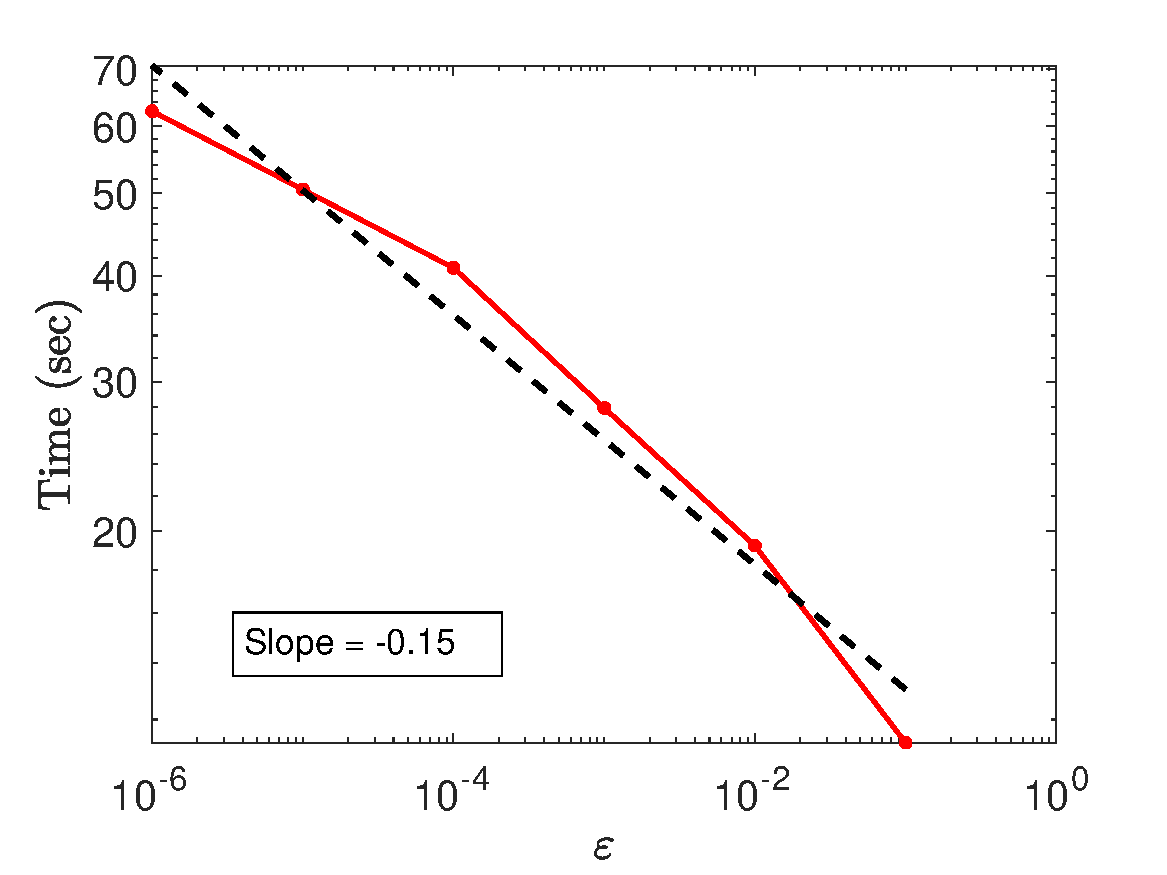
\includegraphics[scale=0.42]{./figures/fig_times_varEps_NC1}
	\caption{(Left) $L_2$ and $\infty$-norms of the velocity in the entire fluid domain. (Right) Time, in second, for one time-step computation with various $\varepsilon$.}
	\label{fig_errNorms_varEps_NC1}
\end{center}
\end{figure}
\clearpage
\subsection{Computation time results}
The data is stored in \verb+data_fmm_t10_varNx_mm5+ and the plot is generated by \verb+plot_time_varNx2+. We use the following values to compare the FMM3D computation to the previous results.
\begin{framed}
	\begin{itemize}
	\item \verb+Nx = [2^3, 2^4, 2^5, 2^6]+
	\item \verb+Ny = Nx, Nz = 2Nx+
	\item Fluid domain size: $[-20, 20] \times [-20, 20] \times [-40, 40]$
	\item \verb+dt = 0.1+
	\item \verb+Nt = 10+
	\item Pe = 50
	\item \verb+NC = 125+ (Cube shape)
	\end{itemize}
\end{framed}
The left one in figure \ref{fig_time_fmm_sum} is the previous results we observed, showing that the velocity evaluation using original SLP code is dominating the computation time. With the same setting, the right plot shows that we can reduce the time almost 10 times by applyting the FMM3D. We yet introduced the quadrature error, but make sure to be smaller than the corner error. 
\begin{figure}[ht]
	\begin{center}
		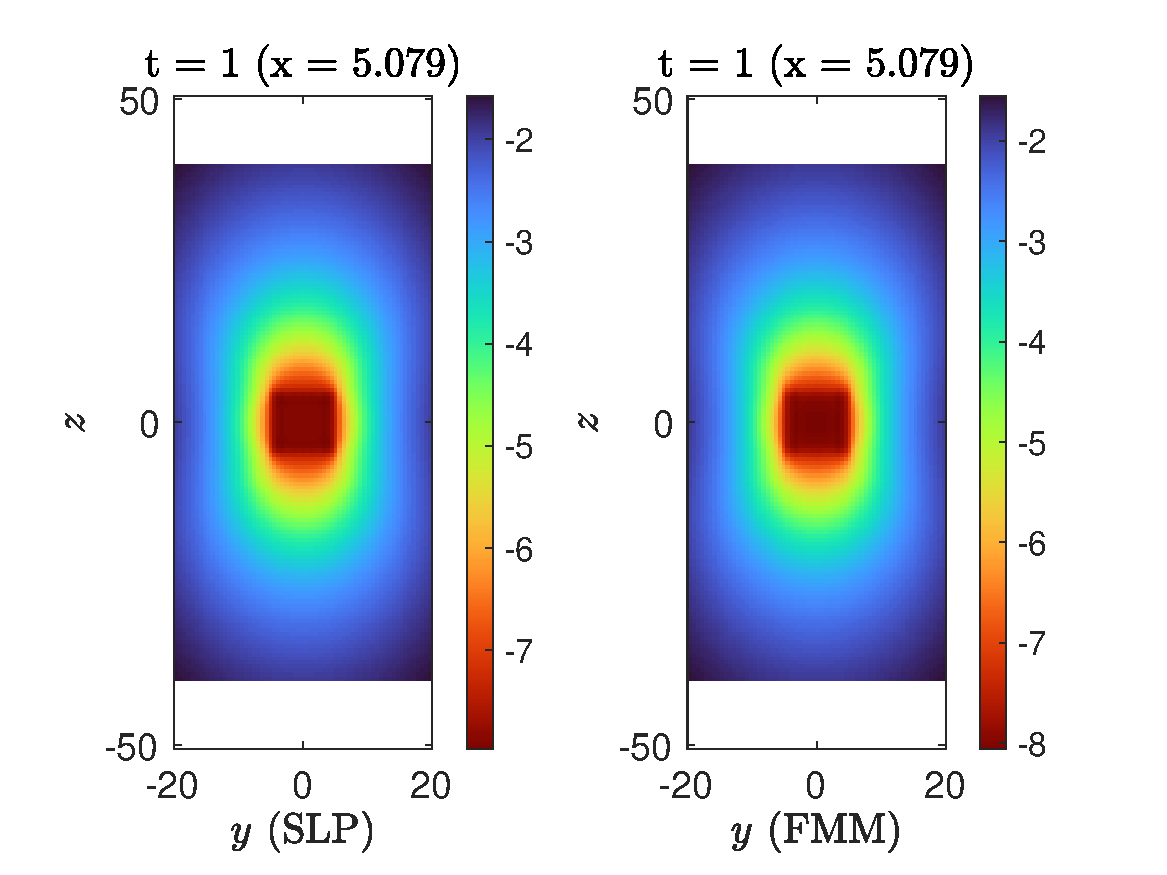
\includegraphics[scale=0.42]{./figures/fig_vel_mm5_t1}
		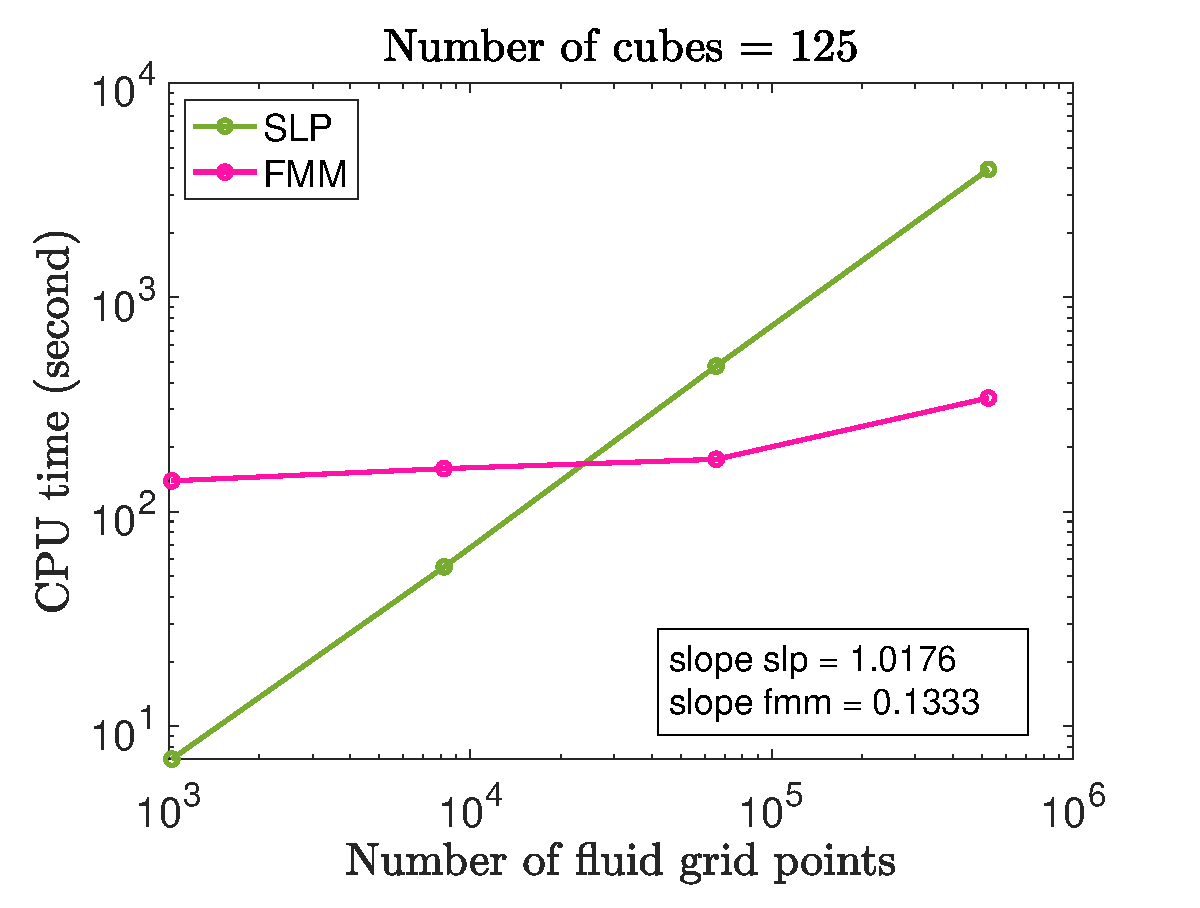
\includegraphics[scale=0.4]{./figures/fig_time_both_mm5_Nt10}
	\caption{(Left) Sample velocity plot at $t=1$ with $Nx = 2^6$. (Right) CPU time with an aggregate made with 125 cubes for 10 time steps. The Pinnacles is used.}
	\label{fig_vel_mm5_t1}
\end{center}
\end{figure}
\clearpage
On January 27, 2023, we decided to check in the timing and memory capacity to use the Pinnacles. I am going to test both SLP and FMM versions, separately, just to make sure if FMM is converging to the correct velocities. Here are the paratmesters we are going to use for this experiment:
\begin{framed}
	\begin{itemize}
	\item \verb+NC = [50, 100]+ (Random shape {\color{red}$\rightarrow$ check the Nf}) 
	\item \verb+Nx = [60, 120]+
	\item \verb+Ny = Nx, Nz = 2Nx+
	\item Fluid domain size: Make $\Delta x =\Delta y = \Delta z = 1$.
	\item $\Delta t = 0.5$
	\item \verb+Nt = 100+ (Final time would be 50.)
	\item Pe = 0.5 ( = $\Delta t$)
	\item {\color{blue} Save at 1) the final time only AND 2) every time step: velocity, C, $U_a$ with location, $\Omega$, $\theta$ (rotaion angle)}
	\end{itemize}
\end{framed}

\clearpage
Figure \ref{fig_time_fmm_sum} is Dec. 2022 results.
\begin{figure}[ht]
	\begin{center}
		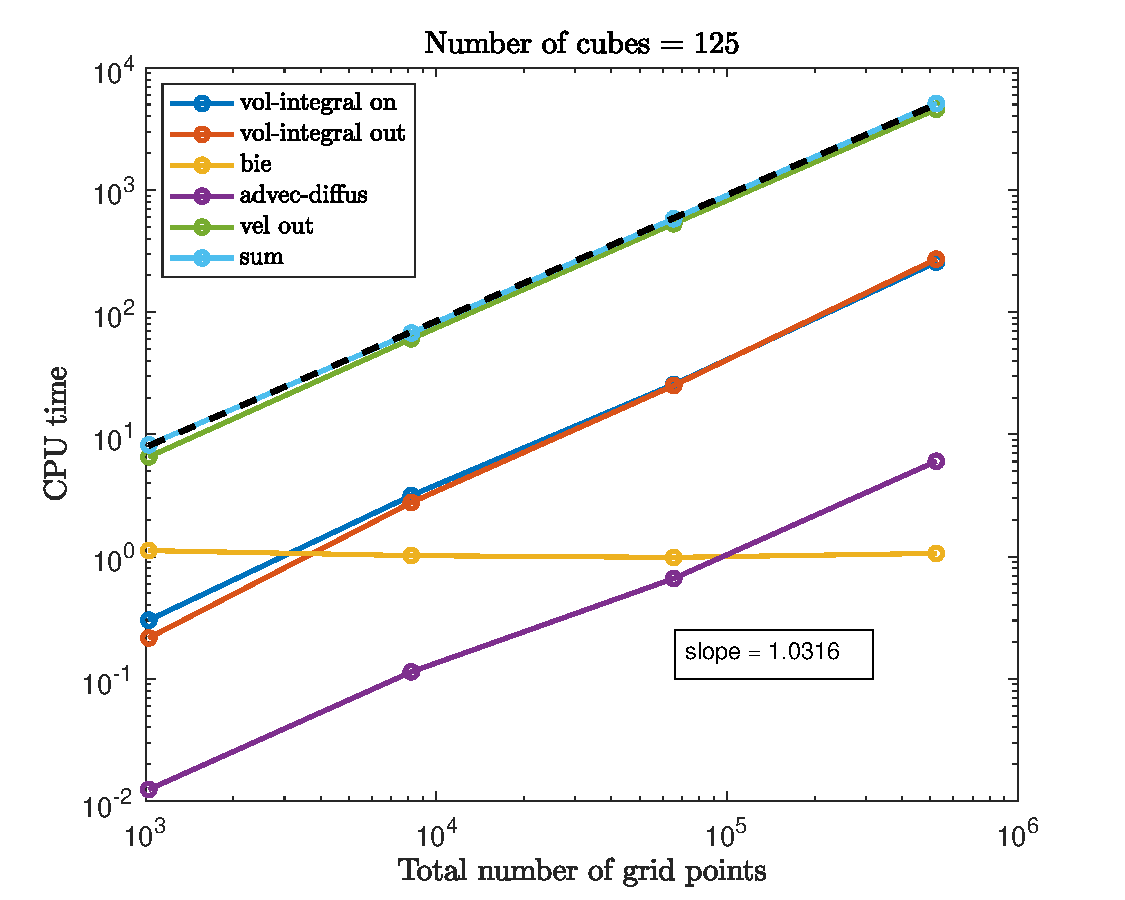
\includegraphics[scale=0.45]{./figures/fig_time_varNx5}
		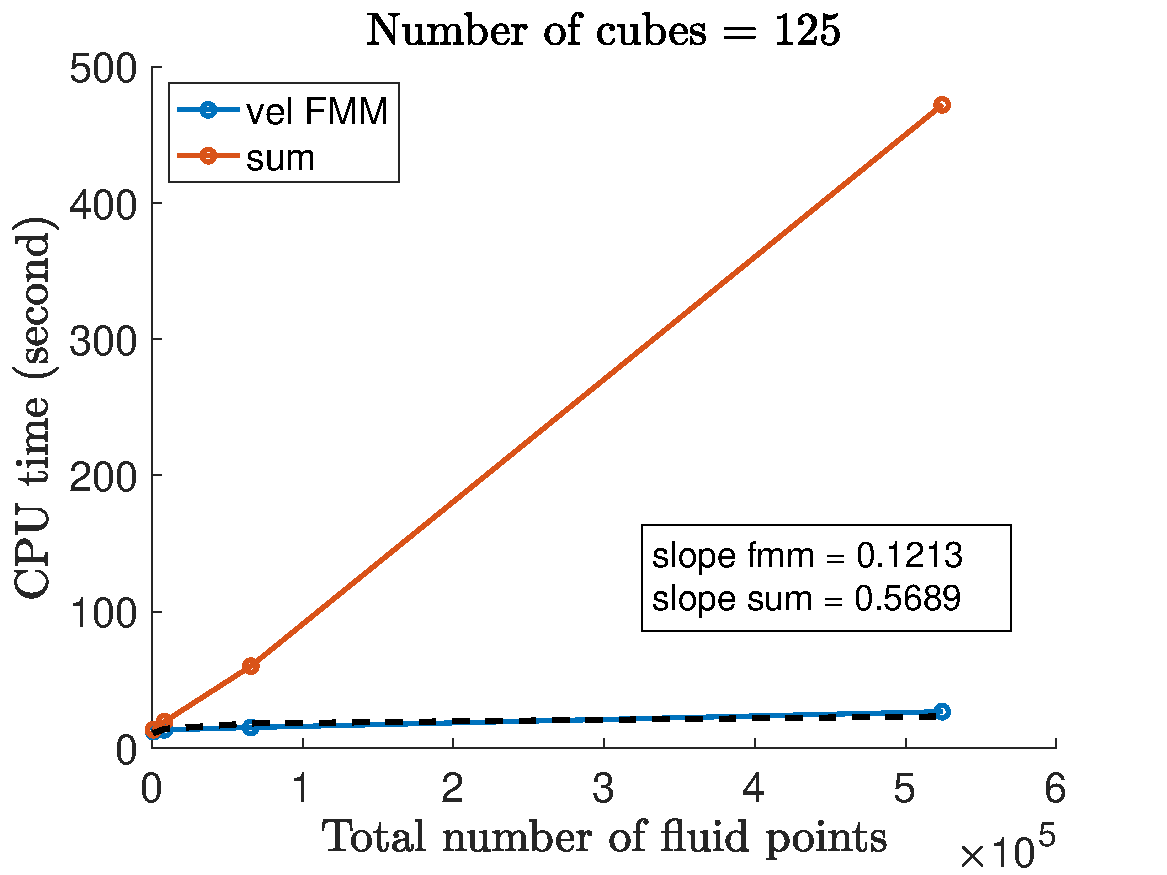
\includegraphics[scale=0.45]{./figures/fig_time_fmm_sum}
	\caption{CPU time with an aggregate made with 125 cubes for 10 time steps.}
	\label{fig_time_fmm_sum}
\end{center}
\end{figure}

% \begin{figure}[h]
% 	\begin{center}
% 		\vspace{0.5cm}
% 		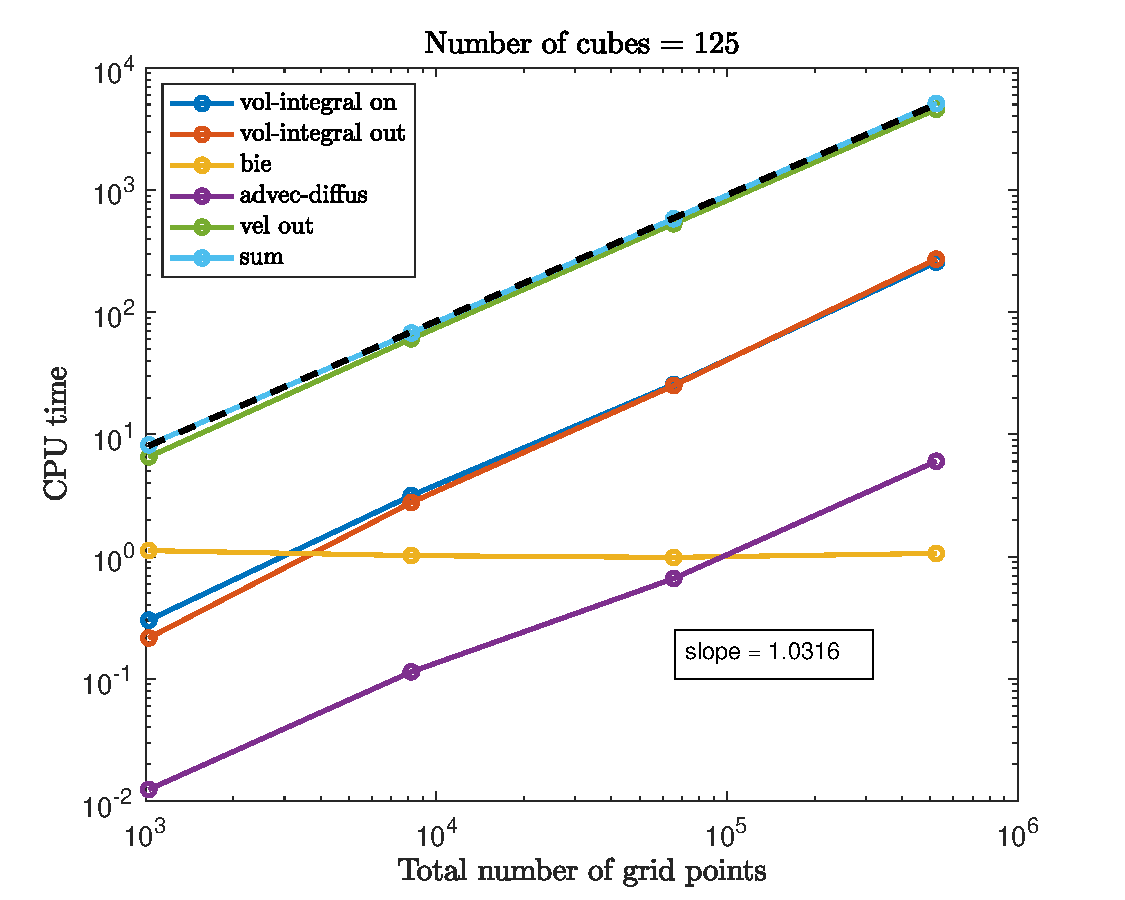
\includegraphics[scale=0.5]{./figures/fig_time_varNx5}	
% 	\caption{Number of cubes is 125.}
% 	\label{fig_time_varNx5}
% \end{center}
% \end{figure}
\begin{comment}
\clearpage
\begin{itemize}
	\item How did you code up exactly to use FMM3D?
	\item you may introduce index notations for this"  $i,j = 1,2,3$ works twice = 18 times  
	\item What is the main difference between volume integral and this surface integral?
	\item {\color{red} We expect to use total 18 times of FMM3D library to compute the entire velocity field.$\rightarrow$ why?}
\end{itemize}
In order to validate the code, measure the error size, and check the computation time, we consider a homogeneous case.
Error plots - compare the $U_a = -0.3470$ values.
\begin{figure}[h]
	\begin{center}
		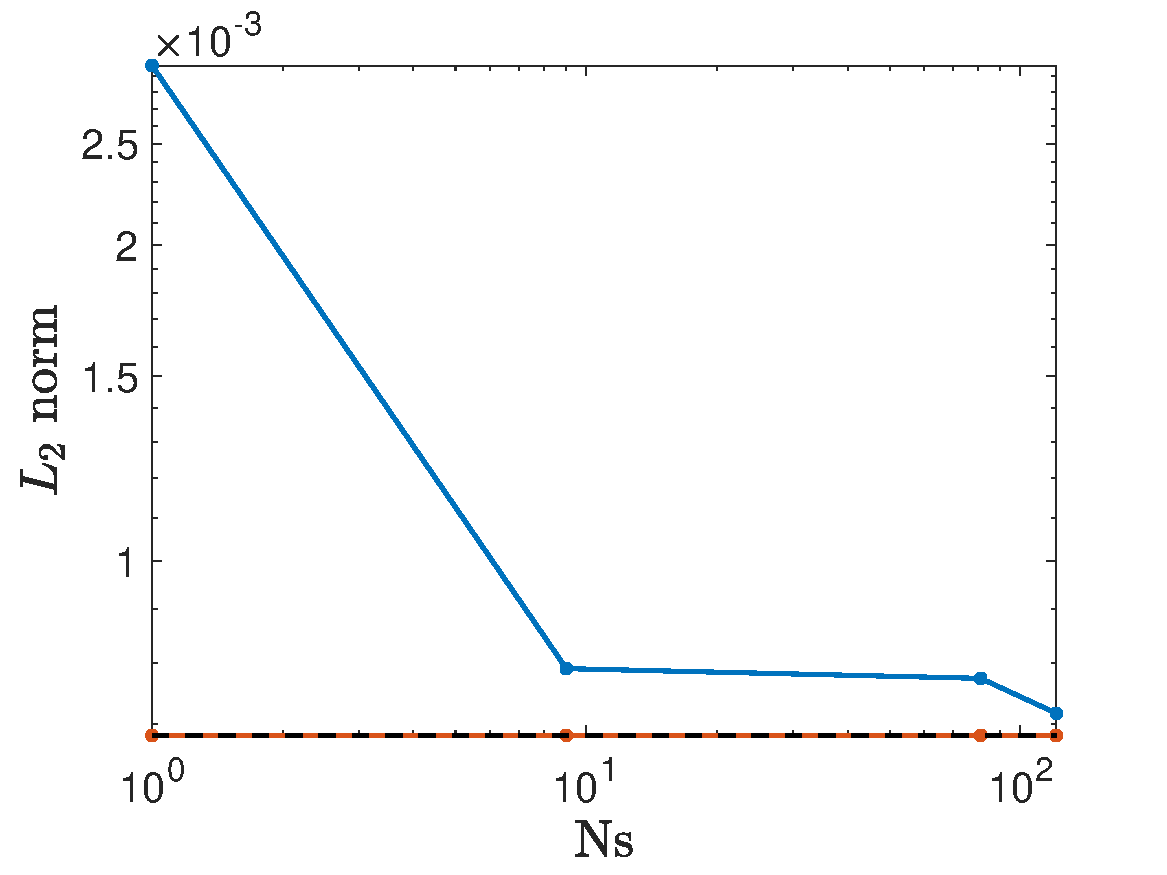
\includegraphics[scale=0.4]{./figures/fig_cornerErr_L2}
		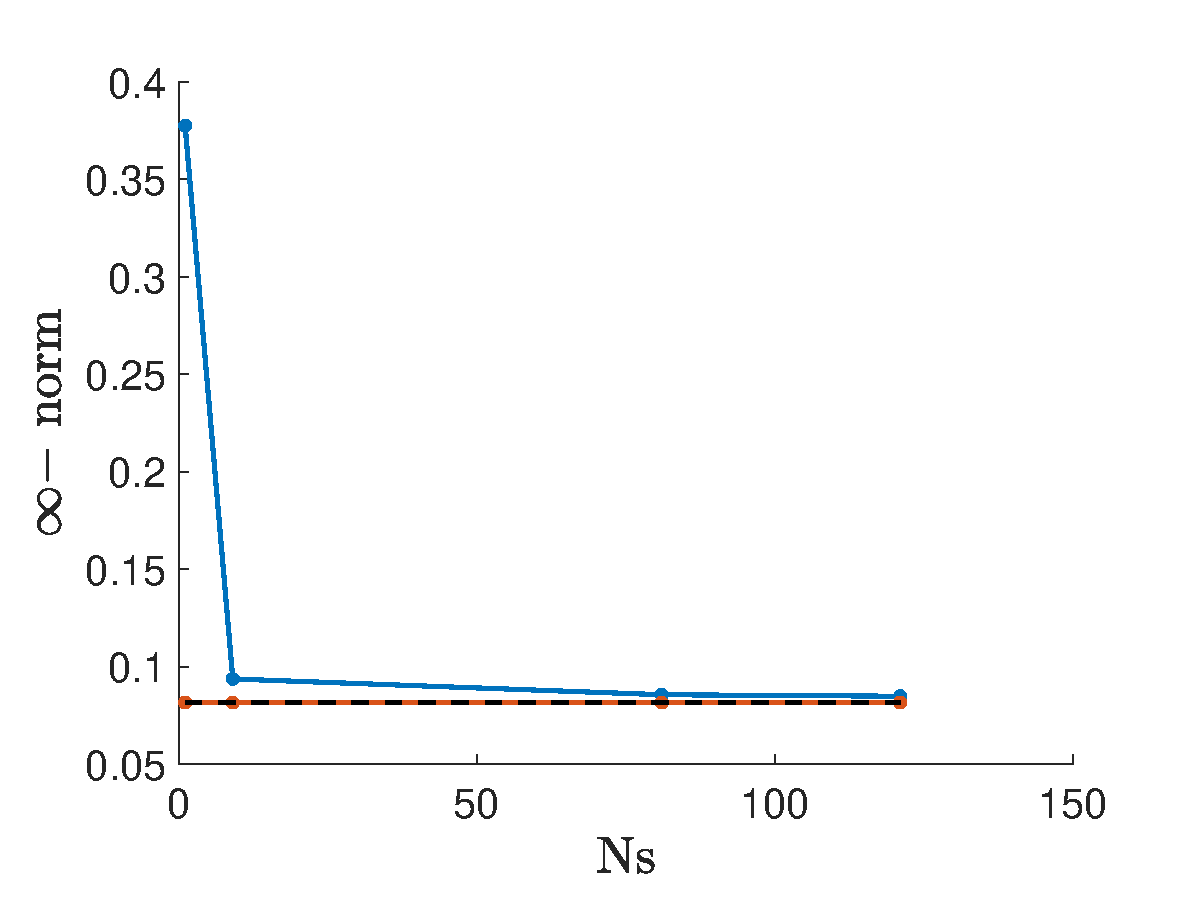
\includegraphics[scale=0.4]{./figures/fig_cornerErr_inf}
	\caption{(Left) Velocity plot of one face. 1 point is used to approximate the surface integral of $G$ kernel using FMM. (Right) $11^2$ point is used to approximate the surface integral of $G$ kernel using FMM. }
	\label{fig_cornerErr}
\end{center}
\end{figure}
\end{comment}
%Rotation---------------------------------------------------


\section{Numerical simulation results}
To somewhat justify our tiny stability issue, we compare the results between two different time step sizes: $\Delta t = 0.25 , \ 0.5$.
\begin{figure}[ht]
	\begin{center}
		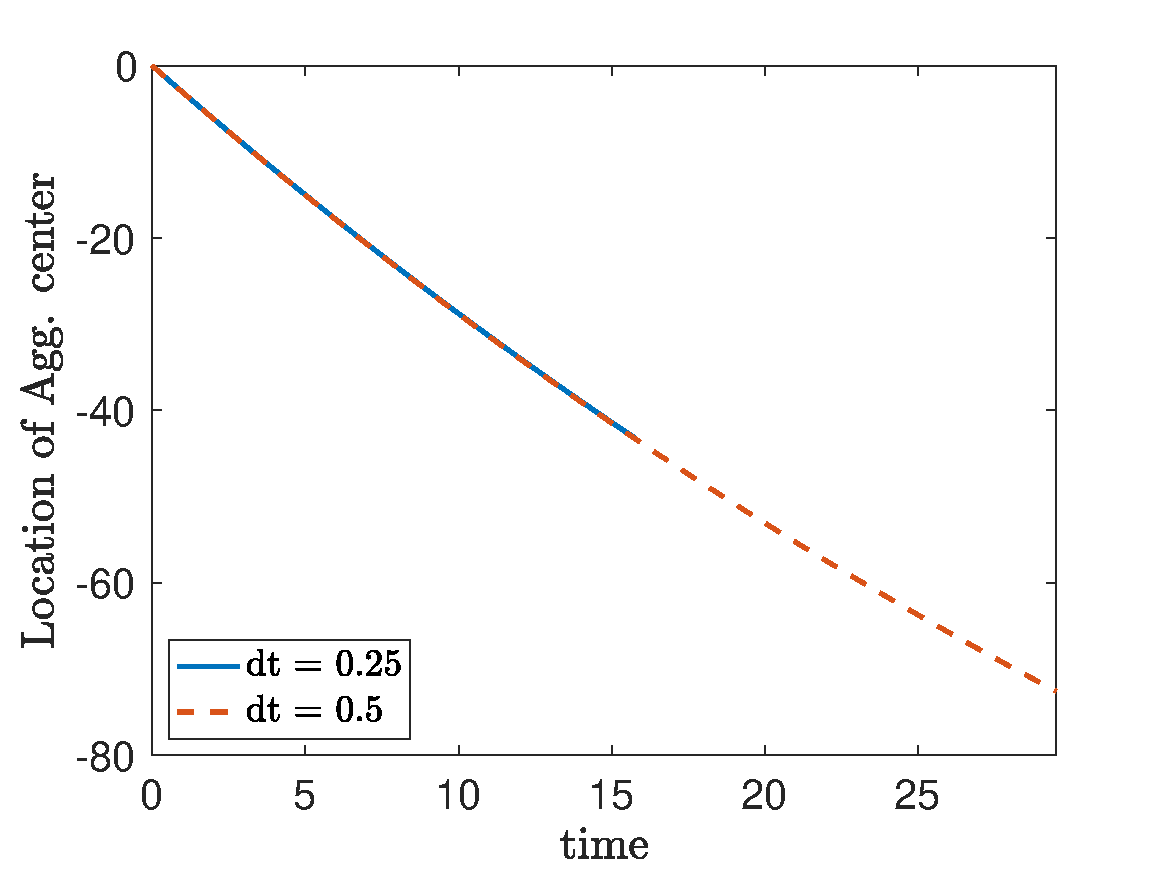
\includegraphics[scale=0.33]{./figures/fig_NC50_compare_dt_cm3_all}
		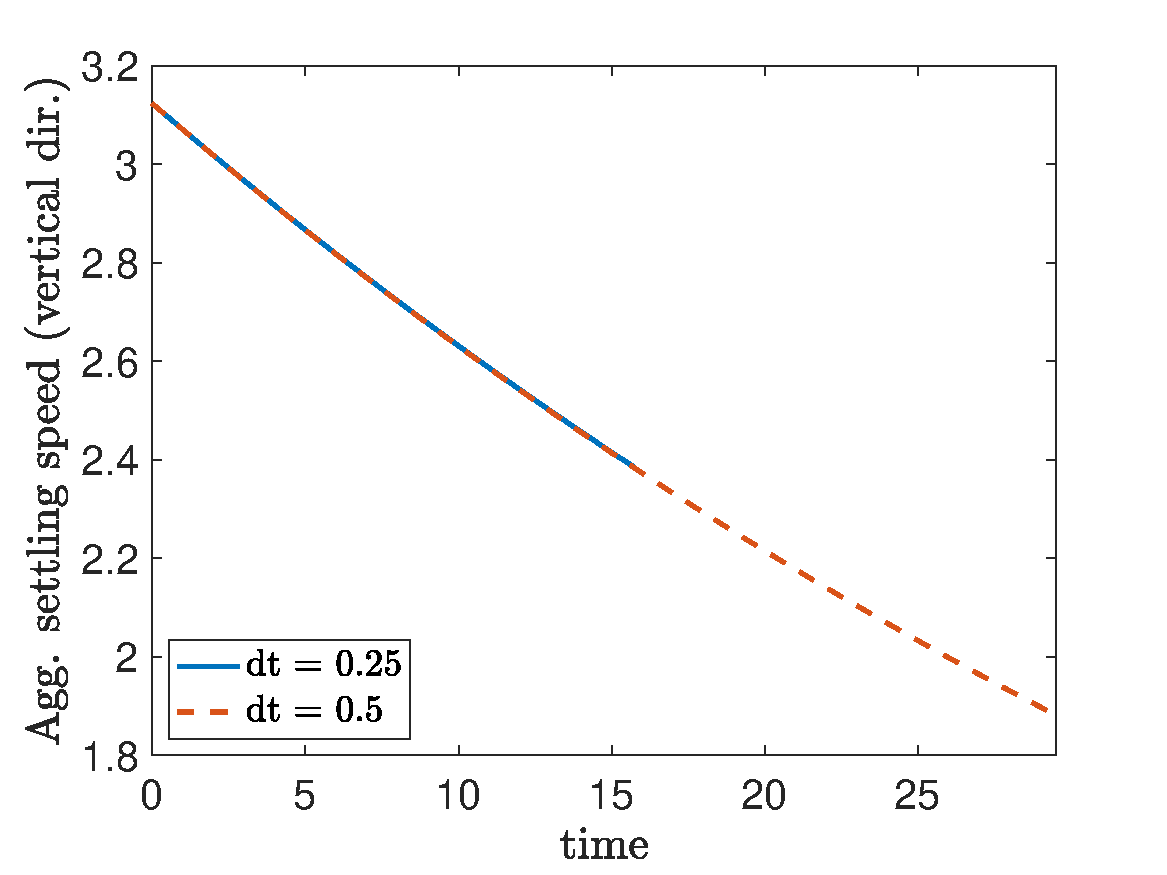
\includegraphics[scale=0.33]{./figures/fig_NC50_compare_dt_Ua3_all}
		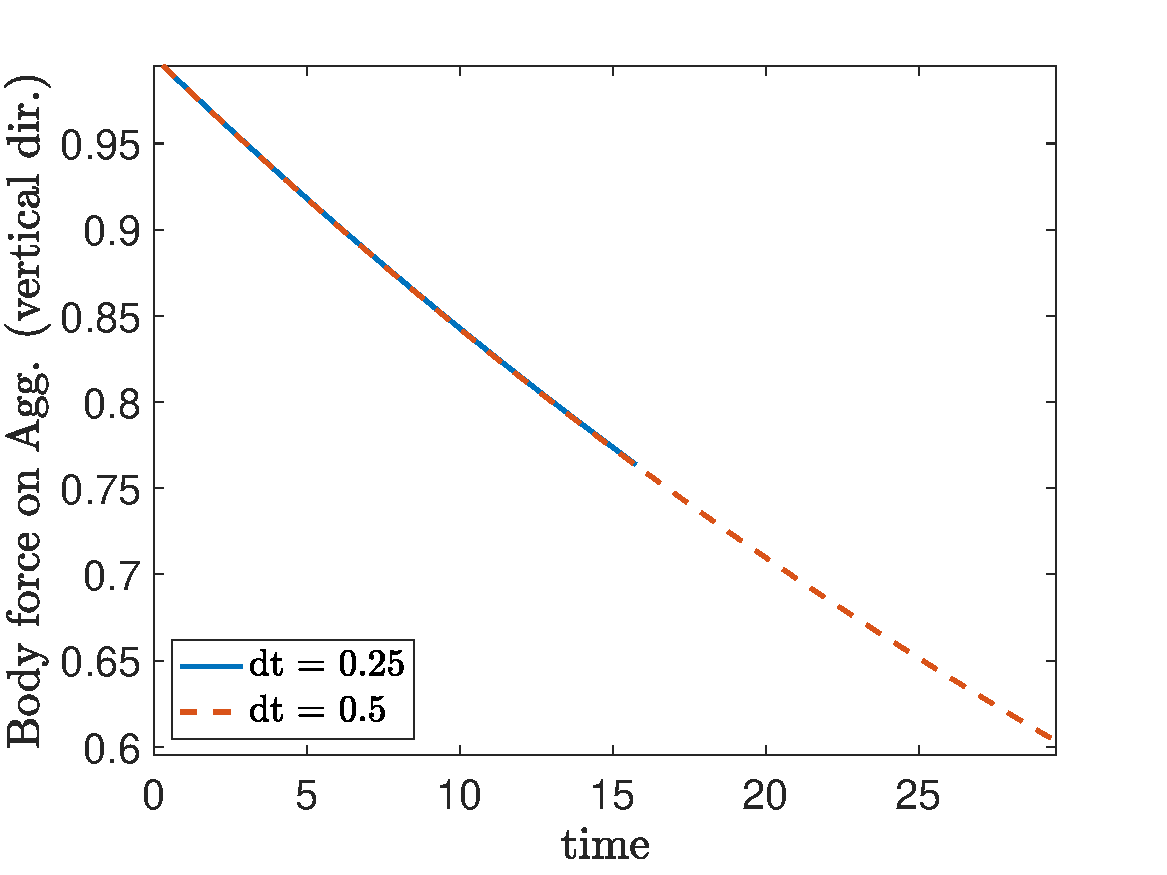
\includegraphics[scale=0.33]{./figures/fig_NC50_compare_dt_Fo3_all}
		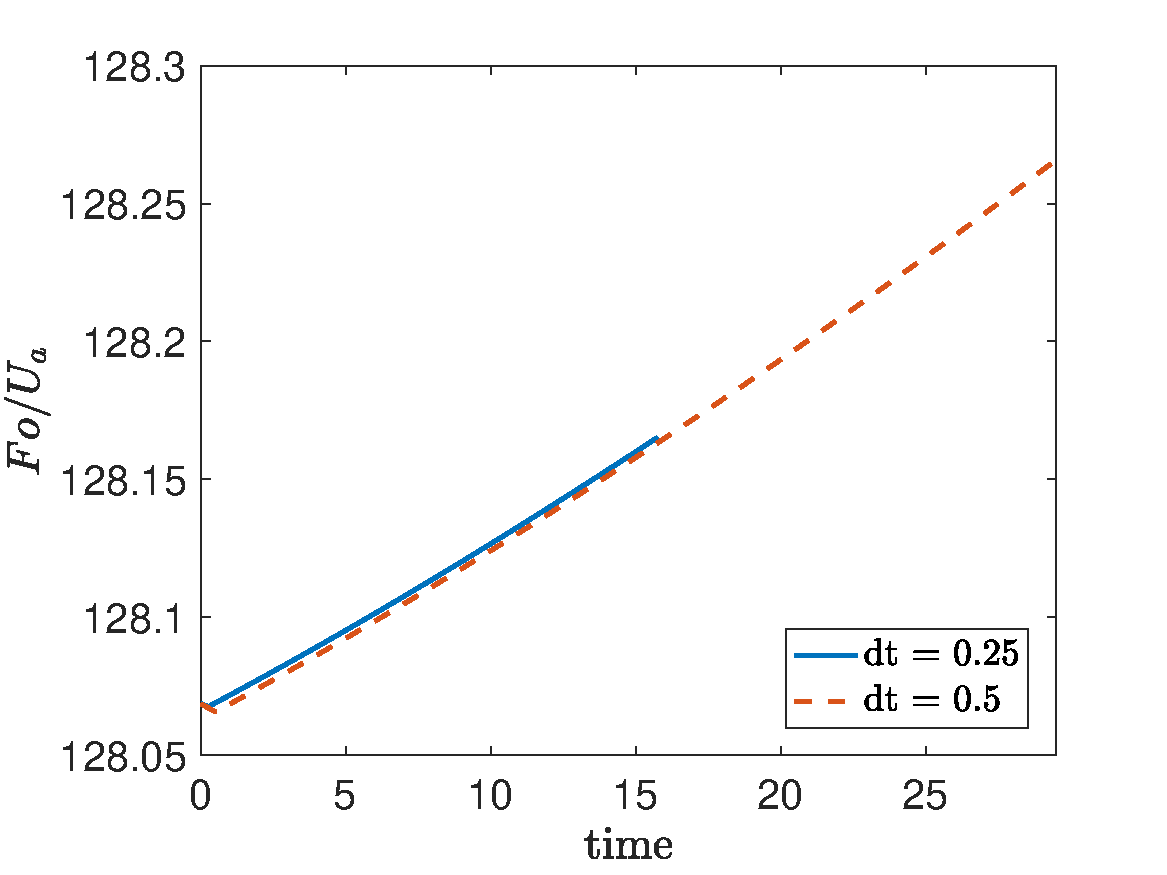
\includegraphics[scale=0.33]{./figures/fig_NC50_compare_dt_UaFo3_ratio}
		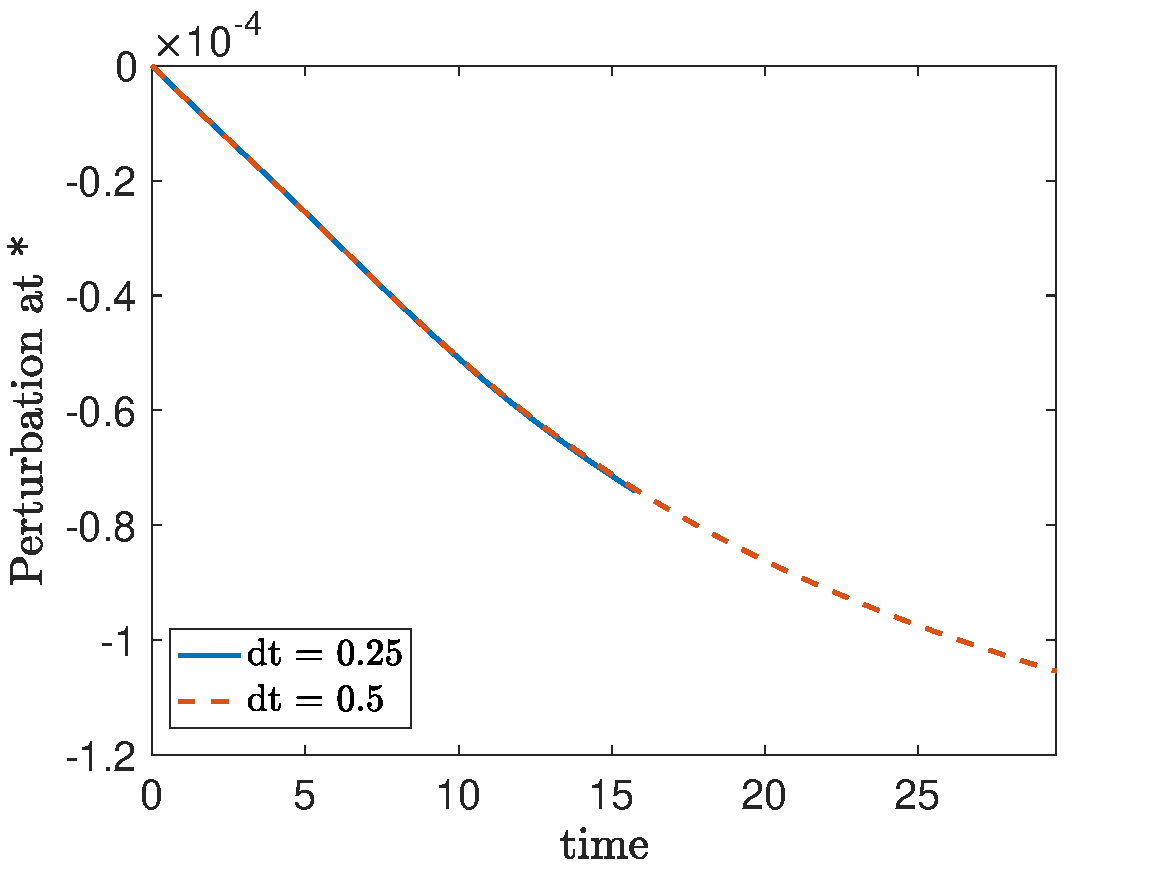
\includegraphics[scale=0.33]{./figures/fig_NC50_compare_dt_C_all}
	\caption{Compare two cases: }
	\label{fig_NC50_compare}
\end{center}
\end{figure}
\section{Discussions}